\cotefile{13}
\scanpage{2}
\begin{flushright}
\uline{Groupe de Hodge}\\
\uline{Lettre à Mumford}
\end{flushright}
% archive sheet number: 1



\scanpage{4}
$G$ groupe algébrique sur $\mathbb{Q}$

\[
\unsure{\mathbb{S}|\mathrm{S}}=\prod_{\mathbb{C}/\mathbb{R}}G_{m\,\mathbb{C}},\quad
\text{donc}\quad \mathbb{S}(\mathbb{R})\simeq\mathbb{C}^{*}.\quad
\text{Soit }\underset{\substack{\Vert\\
\operatorname{Ker}(\mathrm{Norme}:\mathbb{S}\to G_{m\,\mathbb{R}})}}{\mathbb{U}}\subset\mathbb{S}
\]

$\operatorname{Rep}(\mathbb{S})\approxeq$ catégorie des vectoriels réels $V_{\mathbb{R}}$, avec bigraduation sur $V_{\mathbb{C}}=V_{\mathbb{R}}\otimes_{\mathbb{R}}\mathbb{C}$,
\[
V_{\mathbb{C}}\simeq\coprod_{p,q}V_{\deleted{\unsure{p,q|\mathbb{C}}}}^{p,q}
\]
\margin{\uline{NB}\quad $\lambda\in\mathbb{C}^{*}\simeq\mathbb{S}(\mathbb{R})$ opère sur $V^{pq}$ par $\lambda^{p}\bar{\lambda}^{q}$}
satisfaisant la condition
\[
V^{p,q}=\overline{V^{q,p}}.
\]

L'hom canonique $G_{m\,\mathbb{R}}\xrightarrow{i}\mathbb{S}$ correspond à la graduation totale

\diagram{\begin{tikzcd}[ampersand replacement=\&]
\operatorname{Rep}(G) \arrow[r,"\text{oubli}"] \&
\operatorname{Modf}(\mathbb{Q}) \arrow[r,"\otimes_{\mathbb{Q}}\mathbb{R}"] \&
\operatorname{Modf}(\mathbb{R}) \arrow[r,"\otimes_{\mathbb{R}}\mathbb{C}"] \&
\operatorname{Modf}(\mathbb{C})
\end{tikzcd}}

La donnée sur le foncteur composé d'une bigraduation
\[
V_{\mathbb{C}}\simeq\coprod_{p,q}V_{\deleted{\mathbb{C}}}^{p,q}
\]
\margin{i.e. d'une préstructure de Hodge, compatible avec la structure sur $\mathbb{Q}$ donnée, et fonctorielle en l'objet de $\operatorname{Rep}(G)$}
satisfaisant
\[
V^{p,q}=\overline{V^{q,p}}
\]
équivaut à la donnée d'un hom
\[
\mathbb{S}\xrightarrow{j}G_{\mathbb{R}}
\]
Si on se donne un hom [central]
\[
i:G_m\rightharpoonupG.\;,
\]
i.e. une graduation :
\[
V=\coprod_n V^n
\]
sur le foncteur oubli \unsure{$w$|$\omega$}, alors la condition
\[
V^n_{\mathbb{C}}=\coprod_{p+q=n}V^{p,q}
\]
% archive sheet number: 3



\scanpage{5}
équivaut \unsure{à|a} la condition
\[
j\mid G_{m\,\mathbb{R}}=i_{\mathbb{R}}\tag*{(a)}
\]

Pour la suite, $i$ est supposé donné, \deleted{\unsure{Considérons} \unsure{un} $j$ compatible avec $i$ au sens précédent.}\inserted{de $\overline{m}$ qu'un} objet inversible \inserted{$\mathbb{Q}(-1)$} de $\operatorname{Rep}(G)$ à isom près, i.e. un hom \unsure{$\varepsilon$}
\[
\varepsilon:G\longrightarrow G_m
\]
On a alors, pour un $j$ donné, que $\mathbb{Q}(1)$ est de bidegré $(1,1)$ si et seulement si on a les conditions
\[
\varepsilon j(\lambda)=\lambda^2\quad\text{si }\lambda\in\mathbb{R}^{*},\quad
\deleted{\unsure{j\mathbb{U}=1}}\quad
\varepsilon(j(u))=1\quad\text{si }u\in\mathbb{U}\tag*{(*)}
\]
i.e.
\[
\varepsilon j\deleted{\unsure{\mathbb{S}|j}}=\mathrm{Norme}:\unsure{\mathbb{S}|\mathrm{S}}\longrightarrow G_{m\,\mathbb{R}}\tag*{(b)}
\]
On suppose fixé $i$ et $\varepsilon$ satisfaisant \deleted{\unsure{$(a)$}}\inserted{$\varepsilon i(\lambda)=\lambda^2$}, et on s'intéresse aux $j$ satisfaisant a) et b).

\inserted{Soit $j$ donné.} Cherchons, pour $V\in\operatorname{Ob}\operatorname{Rep}(G)$ donné\inserted{ de degré $p$}, \unsure{d'où|D'où} structure de Hodge sur $V_{\mathbb{C}}$, (ou sur $V_{\mathbb{R}}$) quelles sont les \deleted{polarisations de cette structure de Hodge, provenant}\inserted{formes de $R(G)$}
\[
V\times V\xrightarrow{\varphi}\mathbb{Q}(-p)
\]
qui définissent une \uline{polarisation} des structures de Hodge correspondantes. Ce sont celles qui satisfont \unsure{sur|une} la condition que
\[
\varphi_{\mathbb{R}}(x,Cy)\quad\text{forme \inserted{\uline{symétrique}} \uline{définie positive sur} } V_{\mathbb{R}}\times V_{\mathbb{R}}\tag*{(**)}
\]
% archive sheet number: 4



\scanpage{6}
où $C\in\unsure{\mathbb{S}|\mathrm{S}}(\mathbb{R})\simeq\mathbb{C}^{*}$ correspond à l'élément $\sqrt{-1}$ de $\mathbb{C}^{*}$.

[Ceci implique que $\varphi$ est alternée si $n$ impair, symétrique si $n$ pair]
\margin{\uline{NB} Soit $G'=\operatorname{Ker}\varepsilon$, \deleted{\unsure{On a} $\unsure{j(G_m)}$}, alors $G$ est \deleted{\unsure{un quotient de}} $\simeq G'\mathop{\times}\limits_{\mathbb{Z}/2\mathbb{Z}}G_{m\,\mathbb{Q}}$, où $\mathbb{Z}/2\mathbb{Z}\longrightarrow G'$ est induit par $i$. Donc $G$ (avec $i,\varepsilon$) se récupère en connaissant $G'$ et son point d'ordre 2 $i(-1)=\eta$. La donnée de \tikz[baseline=-.25ex,x=1ex,y=1ex]{\draw[line width=.5pt] (0,2.1) -- (0,.18) .. controls (0,-.12) and (.63,-.18) .. (.48,.12) .. controls (.40,.28) and (.18,.23) .. (0,.14);}}

\uline{Théorème} Pour $j$ donné, \unsure{relié|relé} à $i$ et $\varepsilon$ par condition a) et b), les conditions suivantes \inserted{(i)(ii)(i bis)(ii bis)} sont équivalentes et impliquent (iii) :

(i) Pour tout $V\in\operatorname{Ob}\operatorname{Rep}(G)$, \inserted{de degré $n$,} il existe une forme $\varphi:V\deleted{\unsure{\otimes}}\otimes V\longrightarrow\mathbb{Q}(-n)$ dans $\operatorname{Rep}(G)$ qui définit une polarisation (pour \deleted{\unsure{les}}la structure de Hodge \unsure{associées|associée|associés} à $j$ sur $V$, \unsure{$j$|$]$|$\}$} i.e. en fait : $C=j(i)$]

(i bis) Comme (i), mais \deleted{\unsure{avec}} pour des $V_{\alpha}$ donnés seulement \inserted{comme module sur $G'$}, \deleted{qui engendrent}\inserted{et} tels que \deleted{\unsure{les}} l'hom $G\longrightarrow\underline{\mathrm{Aut}}_{\mathbb{Q}}(V_{\alpha})$ soit injectif. De plus, on suppose $G'$ réductif i.e. $G$ réductif

(ii), \deleted{\unsure{(ii bis) Le centralisateur de}} Comme (i), (i bis), mais avec $G$ remplacé par $G_{\mathbb{R}}$, et $\operatorname{Rep}(G)$ par $\operatorname{Rep}(G_{\mathbb{R}})$.

(iii) \inserted{\deleted{\unsure{$G$}} $G'_{\mathbb{R}}$ est réductif, et si $K(\deleted{\unsure{j}})$ est} Le centralisateur de $j(C)$ \inserted{(noté encore $C$)} dans $G_{\mathbb{R}}^{\prime\,0}\deleted{\unsure{/i_{\mathbb{R}}(G_{m/\mathbb{R}}^{0})}}$\margin{\unsure{compos. de|composante} \deleted{\unsure{connexe}} topologique}, \inserted{l'image de $K(j)$ dans $G_{\mathbb{R}}^{0}/i_{\mathbb{R}}(\mathbb{R}^{*+})$} est un sous-groupe compact maximal, \deleted{\unsure{le}} i.e. le centralisateur de $C$ dans $G_{\mathbb{R}}^{\prime\,0}$ est un ss-groupe compact \deleted{\unsure{en groupe}}\inserted{maximal.}

% margin note written sideways
\margin{\uline{NB} (iii) équivaut aux conditions :

(iii bis) $G^{\mathrm{ad}}=G/\mathrm{Centre}$ avec le composé \deleted{\unsure{la}} $\mathbb{S}\mathbin{-}G\to G^{\inserted{\mathrm{ad}}}\deleted{\unsure{/\mathrm{Centre}|/G_{\mathrm{cen}}}}$ satisfait à (i)

(iii ter) $\exists$ un quotient \inserted{$G''$} de $G$ par un ss-gpe fini de $G'$, tel que le composé $\mathbb{S}\mathbin{-}G\rightharpoonupG''$ satisfasse à (i)}

\noindent\rule{\linewidth}{0.3pt}

\tikz[baseline=-.25ex,x=1ex,y=1ex]{\draw[line width=.5pt] (.34,2.5) -- (.28,.16) .. controls (-.02,.39) and (-.32,.02) .. (-.10,-.14) .. controls (.11,-.28) and (.29,-.03) .. (.28,.16);}\quad $j:\mathbb{S}\longrightarrow G_{\mathbb{R}}$ \deleted{équivaut} satisfaisant a) et b équivaut à la donnée d'un hom $j':\mathbb{U}\longrightarrow G_{\mathbb{R}}'$ satisfaisant $j'(-1)=\eta$
% archive sheet number: 5



\scanpage{7}
\deleted{Pour tout espace analytique $S$, soit $F(S)$ l'ensemble \inserted{\unsure{quotient} des objets suivants} des \uline{foncteurs} qui, à chaque $V\in\operatorname{Rep}(G)$, associe}

Soit $S$ un espace analytique. Une $G$-\uline{subordination} \inserted{\uline{rigidifiée}} \uline{sur} $S$ est la donnée d'un $\otimes$-foncteur qui, à tout $V\in\operatorname{Ob}\operatorname{Rep}(G)$, associe une structure de famille de Hodge \inserted{mod isogénie} sur $V_{\mathbb{C}}\times S\unsure{\underset{\mathrm{D}}{=}|\underset{\delta}{=}|\underset{\mathrm{Df}}{=}}V_S$ \deleted{polarisables en chaque point,} [i.e. une bigraduation \inserted{analytique \uline{réelle}} sur $V_{\mathbb{C}}\times S$, \inserted{\deleted{\unsure{autres}} avec $V_S^{pq}=\overline{V_S^{q,p}}$,} telle que la $p$-filtration correspondante soit une filtration analytique complexe] et telle que \inserted{a) degré total soit celui défini par $i$ b) $\mathbb{Q}(-1)$ devienne \unsure{St|Sf} \unsure{de H.} de bidegré $(1,1)$, et} \inserted{c)} pour \inserted{$\forall$ $V$ homogène de degré $n$ et} $\forall\,s\in S$, la fibre en $s$ soit polarisable \deleted{\unsure{pour} $\forall$ \unsure{p\textsuperscript{t} fixé}}\inserted{à l'aide d'une forme $\varphi:V\otimes V\to\mathbb{Q}(-n)$ \inserted{qui soit $G$-invariante (NB. si $S$ est connexe, il suffit de l'exiger cette condition en \uline{un} point \deleted{\unsure{$s$}} de $S$, car la forme restera de polarisation partout, puisqu'elle est non dég. partout}}

\deleted{\unsure{Retenant|Retenons}}\inserted{Oubliant pour le moment la condition de} holomorphie de la filtration, on trouve :

a) pour $\forall$ p\textsuperscript{t} $s\in S$, on veut une façon \deleted{de faire} fonctorielle de mettre une structure de Hodge \inserted{(mod isogénie)} polarisable sur les $V\in\operatorname{Ob}\operatorname{Rep}(G)$, i.e. donnée par un $j=J(s):\unsure{\mathbb{S}|\mathrm{S}}\longrightarrow G_{\mathbb{R}}$ satisfaisant les conditions du th, i.e. $j'=J'(s):\mathbb{U}\unsure{\rightharpoonup|\to}G'_{\mathbb{R}}$ satisfaisant $j'(\deleted{\unsure{C}}-1)=\eta$, et tel que $\operatorname{Zent}_{G_{\mathbb{R}}^{\prime\,0}}(j'(s)(C))$ soit compact maximal.

b) Pour $s$ variable, $j'(s)$ dépend de $s$ de façon analytique réelle.
% archive sheet number: 6



\scanpage{8}
Enfin, pour exprimer la condition d'holomorphie de la \unsure{fibration|filtration}, il convient d'introduire, \deleted{sur} sur l'ens \inserted{$\unsure{\mathscr{J}|\mathcal{J}|\gamma}$} des $j$ (ou $j'$) possibles, une structure de \uline{variété} \uline{analytique} \uline{complexe} naturelle, et la condition s'exprime par l'\uline{holomorphie} de l'application
\[
s\longmapstoJ(s):\quad S\rightharpoonup\mathscr{J}.
\]

\deleted{En un \unsure{mot}} Donc l'ens des $G$-subordinations \inserted{rigidifiées} base $S$ s'identifie à l'ens. $\operatorname{Mor}(S,\mathscr{J})$\margin{morph. d'espaces analytiques}. Donc pour $S$ variable, on a un foncteur représentable par $\mathscr{J}$.

\uline{NB} $G(\mathbb{R})$ opère de façon évidente sur $\mathscr{J}$ (mod autom intérieurs) ; les orbites sont \uline{ouvertes}. Donc

\deleted{Soit \deleted{\unsure{$G$ un}} $V$ un $G$-module fidèle, et $V_0\subset V$ un $Z$-module de type fini engendrant $V$. Alors $\forall$ $G$-subordination sur un $S$ définit une structure de Hodge (\uline{pas} mod isog) sur $V_0\times S$, Soit $\Gamma\subset G(\mathbb{Q})$ le stabilisateur de $V_0$.}

les comp. connexes de $\mathscr{J}$ sont de la forme $G(\mathbb{R})^{0}/H(\mathbb{R})\cap G(\mathbb{R})^{0}$, où $H$ est le centralisateur d'un $j:\unsure{\mathbb{S}|\mathrm{S}}\longrightarrow G$ dans $G$ ; ou encore $G'(\mathbb{R})^{0}/H'(\mathbb{R})\cap G'(\mathbb{R})^{0}$, $H'$ le centralisateur d'un $j':\mathbb{U}\longrightarrow G'$ dans $G'(\mathbb{R})^{0}$.
% archive sheet number: 7



\scanpage{9}
Soit $C=\operatorname{Rep}G$ la $\otimes$-catégorie définie par $G$, et $S$ un espace analytique \uline{connexe}, $s\in S$. On veut classifier les $\otimes$-foncteurs
\[
F:C\longrightarrow\text{str. de Hodge \inserted{(mod. isogénie)} sur }S
\]
telles que\tikz[baseline=-.2ex,x=1ex,y=1ex]{\draw[line width=.55pt] (0,2.0)--(0,.13) .. controls (-.30,-.07) and (.32,-.16) .. (.17,.10) .. controls (.13,.21) and (.05,.19) .. (0,.13);}\inserted{\tikz[baseline=-.2ex,x=1ex,y=1ex]{\draw[line width=.42pt] (.10,2)--(0,.16) .. controls (-.26,-.02) and (.37,-.20) .. (.28,.11) .. controls (.23,.25) and (.08,.24) .. (0,.16);}\ a) degré total (rel. à $i$) $=\sum$ degrés partiels b) $\mathbb{Q}(-1)$ donne str. de Hodge de bidegré $(1,1)$, et} c) Pour \deleted{tout $s\in S$ [en \uline{un} $s\in S$, c'est kif kif]} \deleted{et} $V\in\operatorname{Ob}C$, \deleted{\unsure{polarisables en chaque point}} \inserted{$V$ de degré $n$, $\exists\,\varphi:V\otimes V\unsure{\rightharpoonup|\to}\mathbb{Q}(-n)$ tel que $F(\varphi)$ soit une polarisation [en un pt, en tt point, de $S$, c'est kif-kif].}
\margin{De tels objets s'appellent \uline{$G$-subordination sur $S$} (pas néc. \unsure{rigidifiée|rigidifiées}!)}
Composant avec le foncteur fibre en $s$, on trouve un foncteur fibre
\[
C\longrightarrow\operatorname{Modf}(\mathbb{Q}),
\]
et quitte à tordre $G$, on peut supposer qu'on se donné un isomorphisme \inserted{$\varphi$} entre ce dernier et le foncteur oubli.

\deleted{Alors} Soit $\pi=\pi_1(S,\unsure{\xi|\zeta|s})$. Alors $\pi$ opère \inserted{à g.}, sur le foncteur \deleted{\unsure{``fibre}} ``$\mathbb{Q}$-fibre en $s$'' sur la catégorie des str. de Hodge sur $S$, donc opère sur le foncteur composé avec $F$, d'où un premier invariant de $(F,\varphi)$ :
\[
\alpha:\pi=\pi_1(S,\unsure{\xi|\zeta})\longrightarrow G(\mathbb{Q})
\]
Soit d'autre part $\widetilde{S}$ le \unsure{revêtt|revêtmt} universel de $S$ \deleted{\unsure{pointé}} \unsure{marqué} sur $s$ par $\widetilde{s}$. Alors la donnée de $\varphi$ permet de considérer le foncteur $V\longmapsto F(V)\longmapsto F(W)\times_{\unsure{s|S}}\overline{S}$ comme une $G$-subordination de $\widetilde{S}$. Donc on trouve un
% archive sheet number: 8



\scanpage{10}
\unsure{deuxième|\deleted{deuxième}} élément de structure
\[
f:\widetilde{S}\longrightarrow\unsure{\mathscr{J}|\mathcal{J}|\gamma}
\]
Ces deux éléments de structure sont reliés par la condition que $f$ est compatible avec les actions de $\pi$, quand on le fait agir sur $\mathscr{J}$ via $\alpha:\pi\dashvG(\mathbb{Q})\subset G(\mathbb{R})$ et l'action \inserted{à \uline{droite}} de $G(\mathbb{R})$ sur $\mathscr{J}$ (opposée à l'action gauche).

La donnée d'un couple $(F,\varphi)$ équivaut à celle d'un couple $(f,\alpha)$ satisfaisant les deux conditions précédentes.

\deleted{Il faudrait fixer des \uline{réseaux}, et des sous-groupes discrets convenables de $G(\mathbb{Q})$, du type $G(\mathbb{Z})$ commensurable à un tel ....}

Autre façon de présenter les ``choses, \unsure{indépend.ment|indépendamment} du choix d'un point-base $s$ de $S$. \deleted{(\unsure{reprenons|recommençons})}.

\deleted{On dit que $F$ est co} Notons que les foncteurs fibres \inserted{$\Phi_s$ (rel/$\mathbb{Q}$)} sur \deleted{str. de Hodge} $\mathrm{Hodge}(S)$ définis par les divers points $s\in S$ \deleted{\unsure{sont}} \inserted{d'une \unsure{$\overline{m}$|\deleted{c}} composante connexe $S^{i}$ de $S$ sont} isomorphes ; donc aussi les $\Phi_s\circ F$ \inserted{$(s\in S^{i})$}. On dit que \inserted{la $G$-subordination} $F$ est \uline{compatible avec le foncteur} \uline{oubli} \uline{sur} $C=\operatorname{Rep}(G)$ si les $\Phi_s\circ F$ sont isomorphes audit foncteur oubli. Soit alors, pour
% archive sheet number: 9



\scanpage{11}
tout $s\in S$, $P_s$ le \unsure{torseur|torseurs} sur $G(\unsure{\mathbb{Q}|Q})$
\[
 P_s=\operatorname{Isom}_{\otimes}(\unsure{\omega|w}\inserted{\text{foncteur oubli}},\Phi_sF)
\]
Pour $s$ variable, les $P_s$ forment un revêtement principal \inserted{(à droite)} $P$ de $S$, de groupe $\Gamma=G(\mathbb{Q})$. On a tout ce qu'il fallait pour que le \unsure{$\otimes$} composé
\diagram{\begin{tikzcd}[ampersand replacement=\&,column sep=large]
 C=\operatorname{Rep}(G) \arrow[r,harpoon,"F"] \& \operatorname{Hodge}(S) \arrow[r,harpoon,"{V\mathrel{\mapstochar\rightharpoonup} V\times_S P}"] \& \operatorname{Hodge}(P)
\end{tikzcd}}
\deleted{\unsure{ait une struct|ait un struct}} definisse sur $P$ une $G$-subordination, d'où un morphisme
\[
 g:P\rightharpoonup\unsure{\mathscr{J}|\mathcal{J}|\gamma}.
\]
\deleted{Ceci posé,} Ce dernier est compatible avec l'action de $\Gamma=G(\mathbb{Q})$, \inserted{(opérant sur $\mathscr{J}$ à \uline{droite}).} Et la catégorie des \deleted{\unsure{$\otimes$ foncteurs} $F$} $G$-subordinations $F$ sur $S$ compatibles avec le foncteur oubli est équivalente à celle des couples $(P,g)$, $P$ un rév. principal de $S$ de gpe $\Gamma$, $g:P\relbar\mathscr{J}$ un $\Gamma$ morphisme.

Soit $\Gamma_0\subset\Gamma=G(\mathbb{Q})$ un ss-gpe [de \unsure{préférence|préference|preférence}, commensurable à un $G(\mathbb{Z})$]. On appelle $G$-subordination $\Gamma_0$-\unsure{rigidifiée|rigidifiee} sur $S$ la donnée d'une rev. principal $P_0$ de $S$ de
% archive sheet number: 10


\scanpage{12}
\unsure{groupe|gpe} $\Gamma_0$, et d'un \unsure{$\Gamma_0$-hom|$P_0$-hom} de $P_0\longrightarrow\unsure{\mathscr{J}|\mathcal{J}|\gamma}$.

Si $\Gamma_0=\{e\}$, on trouve la notion de $G$-subordination \unsure{rigidifiée|rigidifiee}, si $\Gamma_0=G(\unsure{\mathbb{Q}|Q})$, la notion de $G$-subordination tout court. On peut expliciter la notion par la donnée d'un $F$\inserted{compatible avec $\unsure{\omega|w}$,}, et d'une \deleted{\unsure{sous}} $\Gamma_0$-rigidification de $F$ i.e. un sous-\unsure{fibre|fibré} $P_0$ de $P$, qui soit un \deleted{\unsure{sous}} $\Gamma_{0_S}$-torseur pour l'action naturelle de $\Gamma_{0_S}$\,.....

Pour cette structure, il y a un topos modulaire, qui n'est autre que \deleted{\unsure{$(\mathscr{J},$a|$(\mathscr{J},$}} $(\mathscr{J},$ avec action de $\Gamma_0$ à droite). $\forall$ Le quotient $\mathscr{J}/\Gamma_0$ (avec sa structure d'espace analytique quand $\Gamma_0$ agit proprement comme groupe discret] \deleted{est} joue le role d'une \uline{variété} \uline{de \unsure{modul|moduli|module}} \uline{de niveau} $\Gamma_0$.
% archive sheet number: 11


\scanpage{14}
Algiers Nov.~1, 1965\\
Dear Mumford,\\

I have become aware that I have been a bit rash with the conjectures I told you about Hodge structures, as in the form I stated them they contradict Tates conjecture, \deleted{\unsure{w|a}}which implies the following: if $X$ is a smooth, connected \uline{simply connected} scheme over $\mathbb{C}$, and $\unsure{\mathscr{V}|V}$ a polarized complex analytic family of Hodge structures parametrized by $X^{\mathrm{hol}}$, then $\mathscr{V}$ is ``algebraic'' only if it is a \uline{constant} family. Now it is easy to get examples of $\mathscr{V}$'s, (with $X$ say \uline{any}\unsure{.|{}} homogeneous space under an affine group over $\mathbb{C}$)
% archive sheet number: 13


\scanpage{15}
which are \uline{non} constant, therefore (one hopes!) not ``algebraic'' (as one would like Tate's conjectures to hold).

However, one should try to test if one really can\uline{not} get an algebraic $\unsure{\mathscr{V}|V}$ that way. To start, I wonder if a single Hodge-structure $V$ with \uline{even partial degrees} (therefore giving rise to a ``Hodge-group'' $G$ s.th. $G_{\mathbb{R}}$ is \uline{compact}) can be algebraic \inserted{(except when $G$ is \unsure{comm.|comm})}.

For instance, do you know an algebraic smooth projective surface $Y$ over $\mathbb{C}$, such that ${\unsure{H|H\!V}}^{11}(Y,\mathbb{C})$ is spanned by algebraic cycles, and $\dim H^{0,2}(Y,\mathbb{C})\geq 2$ ?! I would appreciate your comments! \quad Yours\unsure{.|{}}\\
A Grothendieck\\

P.S. What about your $\Theta$-fns, are you going to write a book?
% archive sheet number: 14


\scanpage{16}
P.S. Here what are the modular varieties one gets from considerations of motive-theoretic galois theory.

\[
G\deleted{_{\mathbb{R}}}
= \text{reductive connected alg. group defined over }\mathbb{Q}
\]

\[
\begin{aligned}
U_{\mathbb{R}}={}&\text{dimension one twisted real Torus, with }U_{\mathbb{R}}(\mathbb{R})\\
&\text{identified with the group of complex nbs of}\\
&\text{module }1
\end{aligned}
\]

\[
\begin{aligned}
i_0:U_{\mathbb{R}}\longrightarrow G_{\mathbb{R}}\quad &\text{homomorphism of algebraic}\\
&\text{groups over }\mathbb{R},\ \text{s.th. }i_0(-1)\text{ is}\\
&\text{central, and s.th. \deleted{\unsure{t|a}}the centralisator}\\
&K_{\mathbb{R}}\text{ of }i_0(\sqrt{-1})\text{ is such that}\\
&K_{\mathbb{R}}(\mathbb{R})^{\unsure{0|\circ}}\text{ is \uline{maximal} \uline{compact} in }G_{\mathbb{R}}(\mathbb{R})^{0}.
\end{aligned}
\]

Moreover, for every $\mathbb{R}$-simple component of $G_{\mathbb{R}}$, the corresponding component of $i_0$ is not trivial.

\[
C_{\mathbb{R}}=\text{\uline{Centr}}_{G_{\mathbb{R}}}(i_0)\subset K_{\mathbb{R}}
\]

\[
\deleted{\unsure{\gamma|\mathscr{T}}}Q=G_{\mathbb{R}}/C_{\mathbb{R}}
\]

\[
\text{``Sigel-space''}=\unsure{\mathscr{J}|\mathcal{J}|\gamma}=G(\mathbb{R})^{0}/G(\mathbb{R})^{0}\cap C_{\mathbb{R}}(\mathbb{R})
\overset{\substack{\inserted{\text{(a connected component)}}\\ \deleted{\text{\unsure{open and closed}}}}}{\subset}Q(\mathbb{R})
\]

N.B. $\mathscr{J}$ has a natural complex structure (inherited from \inserted{one on} $Q(\mathbb{R})$ in fact) invariant by operations of $G(\mathbb{R})$. Every linear representation (over $\mathbb{Q}$) of $G$ in\deleted{to} a vector space $V$ (over $\mathbb{Q}$), together with a lattice $V_0$ of $V$, defines a `\uline{complex} \uline{analytic} family \inserted{$\unsure{\mathscr{V}|V}$} of Hodge structures\textsuperscript{\ensuremath{\delta}}\margin{$\delta$\;(\deleted{\unsure{perhaps even|perhaps}} \inserted{necessarily} globally polarizable -- to get a polarization of the family, one picks a ``form of polarization'' $\unsure{\varphi|\phi}$ \uline{on $V$} \deleted{\unsure{,|;}} invariant by $G$).} on $\mathscr{J}$, at least when one fixes a ``total degree'' $n$
% archive sheet number: 15


\scanpage{17}
and assumes that $i_0(-1)$ operates on $V$ as \inserted{homothety} $(-1)^n$. (It is not hard to describe $\unsure{\mathscr{J}|\mathcal{J}|\gamma}$ by universal propert\deleted{ies}y as \deleted{\unsure{being}} representing some functor \inserted{$F(X)$, $X$ \deleted{\unsure{al|an}}complex analytic,} expressing that every $V$ \inserted{as above} should define, in an additive and multiplicative way for varying $V$, a Hodge-structure \inserted{$\unsure{\mathscr{V}|V}$} over $X$). If $\Gamma\subset G(\deleted{\unsure{\mathbb{Q}|\mathbb{R}}}\mathbb{R})$ is the group leaving $V_0$ fixed, then $\Gamma$ operates on $(\mathscr{V},\mathscr{J})$.
% margin note written sideways
\margin{Note that in general $\mathscr{J}$ is \uline{not} riemanian symm., but is a fiber space over a R.S. space, with fibers which are projective complex homogeneous spaces under $K_{\mathbb{C}}$. This implies at least that $\mathscr{J}$ is \uline{simply} \uline{connected}, hence is the univ. covering of $M=\mathscr{J}/\Gamma$ if $\Gamma$ operates freely}

The modular varieties I expect to carry algebraic structure\deleted{\unsure{s}}\unsure{{}|s} \uline{over} $\mathbb{Q}$ (and morally, $\mathbb{Z}$) are the varieties $\boxed{\mathscr{J}/\Gamma}$, where $\Gamma\subset G(\mathbb{Q})\cap G(\mathbb{R}^{\unsure{0|\circ}})$ \deleted{is} is commensurable with $G(\mathbb{Z})$ [for some matrix representation of $G$, \deleted{as} giving a meaning to $G(\mathbb{Z})$]. However, it is possible that one will have to impose on the data some extra conditions, either arithmetic (involving existence of ``Frobenius elements'' in $\deleted{\unsure{G(\mathbb{Q})|G}}\in\unsure{.|{}}\;I(\mathbb{Q})$, $I=G/\text{int. aut.}$),. or geometric \inserted{on $G_{\mathbb{R}}$} (such as: $G_{\mathbb{R}}$ has \uline{no compact factor}). A typical case which fits in the general \deleted{picture} \inserted{description}, but for which I have no evidence so far if $\mathscr{J}/\Gamma$ has
% archive sheet number: 16


\scanpage{18}
an algebro-geometric interpretation in terms of \inserted{moduli for} motives, is the following:

start with a vector space of \unsure{finit.|finite} :\unsure{dimens-|dimension-|dimension} $V$ over $\mathbb{Q}$, with an fundamental bilinear form $\unsure{\varphi|\phi}$ given, symmetric or alternating, take $G=\mathrm{SO}(\varphi)$, take any $i_0:U_{\mathbb{R}}\to G_{\mathbb{R}}$ s.th. $i_0(-1)=\mathrm{id}$ (if $\varphi$ symmetric), $i_0(-1)=-\mathrm{Id}$ (if $\varphi$ \deleted{\unsure{a|o}} skew-symmetric), \deleted{$\unsure{i_0|\mathrm{id}}(\sqrt{-1})\unsure{=|\ne}\unsure{1|{-1}}$} \deleted{$i_0(i)$ non trivial.} \inserted{and a positivity condition of $\varphi$ relative to the bigrading of $V_{\mathbb{C}}$ defined by $i_0$, which I will not write down.}

Then $\unsure{\mathscr{J}|\mathcal{J}|\gamma}$ is a direct generalization of Siegel's half-plane, and classifies all Hodge-structures \deleted{\unsure{under}} with underlying $\deleted{\unsure{V|Q}}\mathbb{Q}$-vector space $V$, \deleted{\unsure{(|a}} i.e. all bigradings of $V_{\mathbb{C}}$, \deleted{\unsure{having}} \inserted{satisfying} the usual symmetry condition for complex conjugation, which are compatible with $\varphi$ (i.e $\varphi$ is a polarization), and for which the $\dim V_{\mathbb{C}}^{pq}$ have given values . (depending on the weights of $U_{\deleted{\mathbb{R}}\mathbb{C}}$ operating on $V_{\mathbb{C}}\ \ldots$). The trouble is that, \deleted{\unsure{if|of}} as these special types of $\mathscr{J}$, $\mathscr{J}/\Gamma$ are in a way ``universal'' for all others
% archive sheet number: 17


\scanpage{19}
(namely the $\mathscr{V}$'s considered above are induced from one's on such special type of $\unsure{\mathscr{J}|\mathcal{J}|\gamma}$), if the ``modular family'' $\mathscr{V}$ of Hodge structures on \inserted{such a} $\mathscr{J}/\Gamma$ was ``algebraic'' i.e. came from a relative motive over the complex analytic space $\mathscr{J}/\Gamma$, \inserted{(or even on some underlying structure of alg. var. over $\mathbb{C}$),} the same would be true for \uline{every} modular family on some $\mathscr{J}/\Gamma$.

Taking the case $G\deleted{_{\mathbb{R}}}(\mathbb{R})$ compact, \deleted{this} and thus $\mathscr{J}/\Gamma=\mathscr{J}={}$complex projective homogeneous space $X$ under $G_{\mathbb{C}}$ by Borel, we would get a \inserted{polarized} motive over the analytic space $\mathscr{J}$ corresponding to $X$. If we admit the \inserted{GAGA} yoga (coming from \inserted{polarized} abelian varieties). that such a family must also be a motive over $X$, \inserted{(or the above strengthening of the original assumption),} we \deleted{would} get a contradiction with Tate's conjectures \unsure{\deleted{as}|\deleted{a}|$\leftarrow$} (\unsure{\uline{bec}|\deleted{bec}}ause $X$ is simply connected, as well known). So I really do not know what to believe!
% archive sheet number: 18


\scanpage{20}

To come back to the general case, maybe I should add that a \uline{necessary} condition for $\unsure{\mathscr{J}|\mathcal{J}|\gamma}/\Gamma$ to be algebraic and the Hodge-structures $\mathscr{V}/\Gamma$ over $\mathscr{J}/\Gamma$ algebraic too, is (\uline{granting} Tate's and Hodge's conjectures): for every $g\in G(\mathbb{R})^{\unsure{0|\circ}}$, and every $\Gamma_0$ of finite index in $G(\mathbb{Z})$, the smallest \inserted{alg.} subgroup $H$ of $G$ such that $H_{\mathbb{R}}$ contains $g[i_0(U_{\mathbb{R}})]g^{-1}$ \uline{and} $\unsure{\Gamma|T}_0$ is $G$ itself.

\deleted{I did \unsure{not|\deleted{not}} try to test directly this condition, even in the case of the \uline{usual} Siegel modular space; if it should be false in that case, as we know that $\mathscr{J}/\Gamma$ \uline{is} algebraic and that so are the $\mathscr{V}/\Gamma$ over it, it would follow that either Hodge's or Tate's conjecture is wrong}

\margin{Question: If $G_{\mathbb{R}}$ is semi-simple without compact factors, is $G(\mathbb{Z})$ always Zariski-dense in $G$\unsure{?!|??}}

By the way, did you make out if for the modular varieties $\mathscr{J}/\Gamma$ of your
\[
\left\{\begin{aligned}
&\text{Boulder talk (which I just read),}\\
&\text{the image of }\mathscr{J}/\Gamma\text{ in the usual Siegel}\\
&\text{modular variety is an algebraic variety,}\\
&\text{or at least constructible?}
\end{aligned}\right.
\]

% archive sheet number: 19


\scanpage{21}
\begin{flushright}\begin{minipage}{.54\linewidth}
Descriptions transcendantes de motifs en car $0$ et de catégories de motifs en car. $0$

\figure{\hspace{.16\linewidth}
\begin{tikzpicture}
 \draw[line width=.6pt,line cap=round] (0,0) .. controls (.55,.01) and (1.25,.03) .. (1.72,.14);
\end{tikzpicture}}

doubles réseaux etc
\end{minipage}\end{flushright}

\vspace{1cm}
\figure{\hspace{.15\linewidth}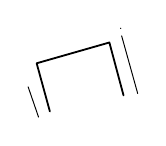
\begin{tikzpicture}[x=.012cm,y=-.012cm,line cap=round,line join=round]
 \draw[line width=.65pt] (24,97) -- (10,46) -- (87,24) -- (102,80);
 \draw[line width=.35pt] (1,71) -- (12,103);
 \draw[line width=.35pt] (100,17) -- (117,78);
 \fill (99,9) circle[radius=.7];
\end{tikzpicture}}

\vspace{3cm}
\figure{\hspace{-.17\linewidth}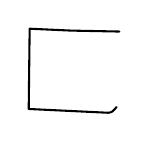
\begin{tikzpicture}[x=.012cm,y=-.012cm,line cap=round,line join=round]
 \draw[line width=.75pt] (98,4) -- (47,3) -- (3,1) -- (2,86) -- (86,90) .. controls (91,90) and (92,87) .. (95,84);
\end{tikzpicture}}
% archive sheet number: 20


\scanpage{23}
\deleted{Dans le cas général (motifs pas nécessairement constants) la connaissance des opérations $\Theta_X$ sur les $V_{\mathbb{C}}$ $(V\in\operatorname{Ob}\mathcal{M})$ implique-t-elle celle des éléments des structures $1^{\mathrm o}$ et $2^{\mathrm o}$, \deleted{ou dans quelle mesure du moins?}}
\margin{\deleted{\uuline{oui}} ??}

\margin{\begin{tikzpicture}
\node[inner sep=1pt,align=left,text width=.93\marginparwidth] (rubrique) {Situation abstraite de la donnée d'une connexion intégrable un foncteur fibre.};
\draw (rubrique.north west) -- (rubrique.south west) -- (rubrique.south east);
\end{tikzpicture}}

\begin{center}\rule[.2ex]{2cm}{.4pt}\end{center}

Considérons une $\otimes$-catégorie $\mathcal{M}$ sur corps $k_0$, soit $K$ une extension de $k_0$. On suppose donné un foncteur fibre à valeurs en $k_0$, \unsure{donc|dans} $\mathcal{M}$. avec ce foncteur fibre est donné par $G$ sur $k_0$, $\mathcal{M}$ s'identifie avec \unsure{``$G$-$k_0$-modules\ldots|$G$-$k_0$-modules\ldots} On veut déterminer les façons de mettre, sur chaque $V\otimes_{k_0}K$ une connexion intégrable \inserted{rel : $K/k_0$}, \uline{fonctorielle} en $V$, \inserted{et ``compatible avec $\otimes$''.}

Or il y en a déjà une $\unsure{\Theta_0|\text{\textcircled{H}}_0}$, déduit des $k$-structures dont on \deleted{\unsure{suppose}} dispose déjà sur chaque $V\otimes_{k_0}K$. Une autre connexion \deleted{\unsure{intégrable}} \inserted{sur $V$} sera donc de la forme
\[
 \Theta_X^V={\Theta_0}_X^V+\omega^V(X)^{\deleted{\unsure{V|x}}}
\]
\unsure{où|ou}
\[
 \omega^V\deleted{\unsure{(X)|\in}}:\operatorname{Dér}_{k_0}(K/k_0)\longrightarrow
 \operatorname{End}_K(V_K\unsure{)}\,\text{est \uline{$K$-linéaire}}
\]
\[
 \Theta_X^V(\varphi)={\Theta_0}_X^V(\varphi)+\omega^V(X)(\varphi)
\]
Si on veut choisir les $\Theta_X^V$ pour tt $V$, de façon compatible avec multiplication, on trouve que \deleted{$\unsure{\omega^V|\omega}\unsure{\Theta_X|(X)}$} $\omega^V(X)$, pour $V$ variable, est une ``dérivation'' du foncteur fibre \deleted{\unsure{donné}}\inserted{$F_K$}, donc défini par un élément de \deleted{Lie} $\mathfrak{g}_K$, où $\mathfrak{g}=\operatorname{Lie}G$. Soit $\omega(X)\in\mathfrak{g}_K$ cet élément.
% archive sheet number: 22


\scanpage{24}
on trouve donc $X\relbar\omega(X):\operatorname{Dér}(K/k_0)\relbar\mathfrak{g}_k$, application $K$-linéaire :
\[
 \omega:\operatorname{Der}(K/k_0)\longrightarrow\mathfrak{g}_K
\]
Si on veut avoir des connexions \uline{intégrables}, il faut écrire de plus la condition d'intégrabilité
\[
 \overbrace{{\Theta_0}_X\omega(Y)-{\Theta_0}_Y\omega(X)}^{\inserted{\mathrm{d}\omega(X\wedge Y)}}
 \deleted{\unsure{+[\omega(X),\omega(Y)]|-[\omega(X),\omega(Y)]}}
 =\omega([X,Y])-[\omega(X),\omega(Y)]
\]
où \deleted{\unsure{$\Theta_0$|On}} $X,Y\in\operatorname{Dér}(K/k_0)$ et ${\Theta_0}_X$, \inserted{${\Theta_0}_Y$} opèrent sur $\mathfrak{g}_K=\mathfrak{g}\otimes_{k_0}K$ via les op. sur $K$.... .

Le plus souvent, on aura en fait
\[
 \omega\in\Omega^1_{K/k_0}\otimes_K\mathfrak{g}_k
 \quad(=\Omega^1_{K/k_0}\otimes_{k_0}\mathfrak{g}_{\deleted{\unsure{K|k}}})
\]
de sorte que $\omega$ provient déjà d'un élément
\[
 \omega_{\deleted{\unsure{K}}k}\in\Omega^1_{k/k_0}\otimes_k\mathfrak{g}_k
\]
où $k$ est une ext. de type fini de $k_0$ (N.B. si $k$ est fixé, $\omega_k$ est uniquement déterminé, si on est en \uline{car. $0$}). La donnée de $\omega_k$ \unsure{revient|équivaut|révient} aussi : la donnée d'un hom $k_0$-linéaire
\[
 \Omega=\check{\mathfrak{g}}\longrightarrow\Omega^1_{k/k_0}\quad(\longrightarrow\Omega^1_{K/k_0})
\]

Nous allons examiner à quelles conditions, \deleted{\unsure{tout hom|tous les hom}} pour $V,W\in\operatorname{Ob}\mathcal{M}$ donnés, \deleted{\unsure{les}} hom \inserted{\uline{de $k_0$-vectoriels}} $u:V_{\deleted{\unsure{K}}}\longrightarrow W_{\deleted{\unsure{K}}}$ \deleted{qui} \inserted{tels que $u_K:V_K\relbar W_K$} commutent \unsure{avec|aux} $\Theta_{\unsure{x|X}}$ $(X\in\operatorname{Dér}(K/k_0))$ \deleted{\unsure{soit|sont}} commutent à $G$, en supposant $G$ connexe ($k_0$ de car. $0$). Il suffit
% archive sheet number: 23


\scanpage{25}
d'écrire que $u_K$ commute \unsure{:|à} $\mathfrak{g}_K$, or par hyp. il commute aux $\omega(X)\in\mathfrak{g}_K$ $(X\in\operatorname{Dér}(\unsure{H|\Pi|K}/k_0)\unsure{]|)}$, Soit $\mathfrak{u}\subset\mathfrak{g}$ le plus petit sous-espace vectoriel de $\mathfrak{g}$ tel que $\mathfrak{u}_K$ contienne les $\omega(X)$. Alors il est clair (alg. linéaire) que \deleted{$\mathfrak{u}$} $u$ commute \unsure{:|à} $\mathfrak{u}$, donc il suffit que $\mathfrak{u}=\mathfrak{g}$ pour pouvoir conclure (N.B. Il suffirait que l'\unsure{algèbre|Algèbre|algébre} de Lie engendrée par $\mathfrak{u}$ dans $\mathfrak{g}$ soit $\mathfrak{g}$, mais en fait on se convainc facilement que $\mathfrak{u}$ est déjà une $\unsure{k|K}$-algèbre de Lie....). On peut $\overline{\mathrm m}$ remplacer $\mathfrak{u}$ par l'algèbre de Lie algébrique qu'elle engendre
% archive sheet number: 24


\scanpage{27}
\begingroup\makeatletter\tagsleft@true\makeatother
\margin{\begin{tikzpicture}
\node[inner sep=1pt,align=left,text width=.93\marginparwidth] (titre) {structure filtrée sur DR et comparaison avec Betti, Hdg...};
\draw (titre.north west) -- (titre.south west) -- (titre.south east);
\end{tikzpicture}}

Soit $k\unsure{\mathrel{\tikz[x=.58em,y=.58em,baseline=0pt,line cap=round]{\draw (.87,.44) .. controls (.60,.70) and (-.03,.34) .. (.04,.17) .. controls (.12,.04) and (.78,.09) .. (1.20,.02); \draw (1.23,.14) -- (1.14,.80) .. controls (1.15,.96) and (.92,.79) .. (.99,1.00) .. controls (1.01,1.08) and (1.05,1.12) .. (1.09,1.13);}}|\subset^{\iota}|\subset}\mathbb{C}$, considérons une catégor. de motifs \inserted{sur $k$,} de type fini \deleted{\unsure{soit}}, soit $\mathcal{M}$. Il y a deux foncteurs fibres naturels,
\[
T_{\mathrm{DR}}:\mathcal{M}\relbar\operatorname{Mod}f(k)\tag*{(1)}
\]
\diagram{\begin{minipage}{\linewidth}
\[
\begin{tikzcd}[ampersand replacement=\&,column sep=1.2em]
T_{B\unsure{\mathrm{dg}|\mathrm{Hdg}|\mathrm{tg}}}:\mathcal{M}\arrow[r]\&
\deleted{\operatorname{Mod}f(\unsure{\mathbb Q|Q})}\ \mathrm{Str.}\ \mathrm{Hodge}\arrow[r]\&
\operatorname{Mod}f(\mathbb Q),
\end{tikzcd}\tag*{(2)}
\]
\end{minipage}}
le deuxième dépendant de l'imm. $k\subset\mathbb{C}$. Le premier a une structure de filtration. De plus, on a un isom canonique
\[
\varphi:T_B\otimes_{\mathbb Q}\mathbb C\xrightarrow{\sim}T_{\mathrm{DR}}\otimes_k\mathbb C\tag*{(3)}
\]
\inserted{compatible aux filtrations des 2 \unsure{mbres|mbrs}}

Soit $G$ gpe des Aut. de $T_B$. Comparant $T_{\mathrm{DR}}$ et $T_B\otimes_{\mathbb Q}k$, on trouve un torseur à droite
\[
P=\unsure{\underline{\operatorname{Isom}}|\underrightarrow{\operatorname{Isom}}}_{\otimes}(T_B\otimes_{\mathbb Q}k,T_{\mathrm{DR}})\tag*{(4)}
\]
sous $G_k$, qui permet de récupérer le foncteur $T_{\mathrm{DR}}$ comme
\[
T_{\mathrm{DR}}=\deleted{T_B\otimes}\ P\overset{G_k}{\times}(T_B\otimes_{\mathbb Q}k).\tag*{(5)}
\]
De plus, \deleted{\unsure{on a un isom.}} l'isom (3) définit un élément canonique
\[
\varphi\in P(\mathbb C)
\]
\margin{\begin{tikzpicture}
\node[inner sep=1pt,align=left,text width=.91\marginparwidth] (note) {La connaissance de $G,P,\varphi$ permet de récupérer ess. $\mathcal M$ avec (1) (2) et (3)};
\draw ([xshift=1pt]note.north west) -- ([xshift=-3pt]note.south west);
\end{tikzpicture}}% slanted

Pour récupérer la structure filtrée sur $T_{\mathrm{DR}}$, \deleted{et} donc la structure de Hodge sur $T_B$ i.e la bigraduation sur $T_B\otimes_{\mathbb Q}C$, il convient d'introduire
\[
T_{\mathrm{Hdg}}\unsure{\in|\mathord{:}}\mathcal M\longrightarrow\operatorname{Mod}\deleted{\unsure{\mathrm{Bi}|\mathrm B}}\mathrm{grad}\,f(k),\qquad T_{\mathrm{Hdg}}=\operatorname{gr}^{*}T_{\mathrm{DR}}.\tag*{(6)}
\]
\inserted{Soit} \deleted{et les deux \unsure{groupes|grpes} de} \deleted{Lie}
\[
\deleted{\unsure{H|K}}\ G'_k=P\overset{G_k}{\times}G_k=\operatorname{ad}(P)\simeq\underline{\operatorname{Aut}}_{\otimes}(T_{\mathrm{DR}})\tag*{(7)}
\]
\deleted{\unsure{Ainsi|Alors}} et
\[
\begin{aligned}
H'\subset G'_k\qquad &\text{ss grpe des $\otimes$-Aut de $T_{\mathrm{DR}}$ respectant}\\
&\text{la filtration et qui induisent l'}\\
&\text{identité sur le gradué associé.}
\end{aligned}\tag*{(8)}
\]
\endgroup
% archive sheet number: 26


\scanpage{28}
\begingroup\makeatletter\tagsleft@true\makeatother
C'est un groupe unipotent, et on peut introduire
\[
Q=\underline{\operatorname{Isom}}_{\substack{\otimes,\,\text{ind. l'ident.}\\\text{sur }\operatorname{gr}^{*}}}(T_{\mathrm{DR}},T_{\mathrm{Hdg}}),\tag*{(9)}
\]
de sorte que $Q$ est un torseur à droite sous $H'$. Posons

\reversemarginpar
\margin{\figure{\begin{tikzpicture}[x=0.42cm,y=0.42cm]
\draw[->] (0.4,-3.3) .. controls (-0.55,-1.5) and (-0.05,-0.6) .. (0.55,-0.45) .. controls (1.3,-0.25) and (2.1,-0.13) .. (2.9,0.25);
\draw (1.5,-3.08) .. controls (1.12,-3.32) and (0.51,-3.05) .. (0.45,-3.3);
\draw (0.52,-3.34) .. controls (0.38,-3.92) and (0.67,-4.08) .. (1.12,-4.04);
\end{tikzpicture}}}
\normalmarginpar
\[
\begin{aligned}
\deleted{\unsure{G''|G'}}\ H''=Q\overset{H'}{\times}H=\operatorname{ad}(H')&\simeq\deleted{\operatorname{Aut}}\ \text{ss-gpe de}\\
&H''=\underline{\operatorname{Aut}}_{\unsure{\ominus|\otimes}}(T_{\mathrm{Hdg}})\ \text{respectant}\\
&\text{la filtration associée}\\
&\text{à la bigraduation,}\\
&\text{et induisant l'identité}\\
&\text{sur gradué}\\
&\text{associé --}
\end{aligned}\tag*{(1\deleted{\unsure{0|1}}\unsure{1|0})}
\]
\[
G''=Q\overset{H'}{\times}G'=\underline{\operatorname{Aut}}_{\ominus}(T_{\mathrm{Hdg}}).\tag*{(10)}
\]
Alors la bigraduation de $T_{\mathrm{Hdg}}$ définit
\[
i_1,i_2:\unsure{\mathbb{G}_{m_k}|G_{m_k}}\relbarG'\tag*{(12)}
\]
satisfaisant
\[
\varepsiloni_1(\lambda)=\varepsilon i_2(\lambda)=\lambda,\qquad \unsure{i_1|i'_1}(\lambda)i_2(\lambda)=\unsure{i|i'}(\lambda).\tag*{(13)}
\]

Ainsi, on obtient les données suivantes

\begin{enumerate}[label=\alph*)]
\item Gpe algébrique $G$ sur $\mathbb Q$, avec \diagram{\begin{tikzcd}[ampersand replacement=\&,column sep=small]\mathbb{G}_m\arrow[r,"i",no head]\& G\arrow[r,"\varepsilon",no head]\& \mathbb{G}_m\ \ldots\end{tikzcd}}
\item Groupe algébrique $G''$ sur $k$, avec \diagram{\begin{tikzcd}[ampersand replacement=\&,column sep=small]G_m\arrow[r,"i''",no head]\& G''\arrow[r,"\varepsilon''",no head]\& G_m\ \ldots\end{tikzcd}}
\item hom $i_1,i_2$ (12) satisfaisant les conditions (13)
\item Torseur \inserted{à g.} $Q$ sous le groupe \inserted{unipotent} $H''$ \inserted{$\subset G''$} défini par $(G'',\unsure{i_1|i_+})$\deleted{\unsure{le|de}}

On considère alors $\deleted{\unsure{Q\overset{H''}{\times}G''=|Q\overset{H'}{\times}G'=}}$
\[
\left\{\begin{aligned}
H'&=H''\overset{H''}{\times}Q=\operatorname{ad}_{H''}(Q)\\
\makebox[0pt][r]{\smash{\raisebox{-.8ex}{\parbox[c]{1.05em}{\figure{\tikz[x=.6em,y=.8em]{\draw[->] (.55,1.4) .. controls (-.30,1.13) and (-.27,.05) .. (.72,-.08);}}}}}\hspace{.25em}}G''&\overset{H''}{\times}Q=P\qquad\text{(tors. à g. sous $G''$)}\\
G'&=G''\overset{G''}{\times}Q:\operatorname{ad}_{G''}(Q)
\end{aligned}\right.
\]
[NB, $Q$ est trivial, donc $G'\simeq G''$ (pas canoniquement], puis
\item Torseur à g. $\unsure{P|\mathord{?}}$ sous $G'$, \deleted{avec un \unsure{isomorphisme|homomorphisme} de \unsure{$G_m\overset{G'}{\times}P$|$G'\overset{G'}{\times}P$}.}
\deleted{On considère alors $G$}
\item Un isom $G\otimes_{\mathbb Q}\unsure{K|k}\simeq G'\overset{\unsure{G'|B'}}{\times}\unsure{P^{*}|P}=\operatorname{ad}_{G'}(P)$ \margin{compatible avec les structures $i,\varepsilon$}
\item[] \deleted{\unsure{g) un|g) Un}} g) Un élément \deleted{\unsure{de|en}} $\varphi\in P(\mathbb C]$, \deleted{\illegible{1}}
\end{enumerate}
\endgroup
% archive sheet number: 27


\scanpage{29}
\inserted{\deleted{Moyennant conjecture de Hodge,}} On \unsure{récupère} $\mathcal M$ comme $\mathrm{Rep}(G)$\inserted{(cf a))}, $T_B$ \inserted{(sans structure de Hodge)} comme le foncteur oubli sur $\mathrm{Rep}(G)$, $T_{\mathrm{DR}}$ comme $\deleted{T_B}P\overset{G}{\deleted{\unsure{\otimes|\circ}}\times}(T_D\otimes_{\mathbb Q}k)$ (cf e), f)), \deleted{la structure} de sorte que $G'\simeq\underline{\mathrm{Aut}}_{\unsure{\ominus|\otimes}}(T_{\mathrm{DR}})$.

\deleted{Alors $Q$ est un bitorseur \unsure{sous|sur} $(G',G'')$ (cf b)c)d))}

Alors on a $H'\subset G'$, un bitorseur $Q$ sur $(H',H'')$, \deleted{deux \unsure{hom.} $i_1,i_2$ \unsure{d|et} \unsure{avec}} et $T_{\mathrm{Hdg}}\simeq T_{\mathrm{DR}}\overset{H'}{\times}Q$, enfin \deleted{$i_1,i_2\colon G_m\mathrel{-}$} $G''\simeq\underline{\mathrm{Aut}}_{\otimes}(T_{\mathrm{Hdg}})$ et $i_1,i_2\colon \unsure{\mathbb G_{m_k}|\mathbb G_{m\,k}}\mathrel{-}G''$ définissant une bigraduation sur $T_{\mathrm{Hdg}}$. Les relations \deleted{\unsure{propr.|prop.}} définissant $H''$ en termes de $i_1$ impliquent que cette bigraduation correspond à une \deleted{\unsure{graduation}} \uline{filtration} de $T_{\mathrm{DR}}$. On en conclut une filtration sur $T_{\mathrm{DR}}\otimes_k\mathbb C$. Or $\varphi$ définit \unsure{un|une} isom. de ce dernier avec $T_B\otimes_{\mathbb Q}\mathbb C$, qui se trouve donc muni d'une filtration.

\uline{Conditions} à imposer aux données a) b) c) d) e) f) g)

\deleted{\illegible{1}} 1) Pour tte repr. (ou une repr. fidèle) $V$ de $G$, la filtration qu'on obtient ainsi sur $V_{\mathbb C}$ \deleted{satisfait} fait de $V$ un module de Hodge\inserted{(condition ouverte)}. 2) Ce dernier est \uuline{motivique}

3) La restriction des scalaires de $\mathbb C$ à $k$ de $V_{\mathbb C}$, déduite de $\varphi\colon T_{\mathrm{DR}}\otimes_k\mathbb C\simeq T_D\otimes_{\mathbb Q}\mathbb C$, correspond à une restriction des scalaires du motif sur $\mathbb C$ défini par la structure de Hodge, grâce à 1). \uline{NB} On ne sait pas expliciter \unsure{2)|3)} et 3) \deleted{\unsure{en termes}} directement en termes des données a) .... !

On trouve alors, \inserted{\uline{si on admet les conjectures de Hodge,}} un hom
% paper watermark, sideways
{\centering \textsc{\unsure{Extra Strong}}\\
\textit{\unsure{Ma}\unsure{in|nn}\unsure{ol|on}\unsure{uy|ny|y} \unsure{1808}}\par}
% archive sheet number: 28


\scanpage{30}
\diagram{\begin{tikzcd}[ampersand replacement=\&,column sep=large,execute at end picture={
\draw ([yshift=1pt]fromgroup.south west) -- ([yshift=-2pt]fromgroup.south west) -- ([yshift=-2pt]fromgroup.south east) -- ([yshift=1pt]fromgroup.south east);
\node[below=3pt,align=center,font=\footnotesize] at (fromgroup.south) {Gpe fond.\\motivique};}]
|[alias=fromgroup]| \Pi(\mathrm{Spec}\,k,\unsure{\xi|\zeta})\arrow[r] \& G
\end{tikzcd}}

L'image \deleted{sur la} de la composante connexe doit être alors le sous-groupe rationnel sur $\mathbb Q$ de $G$ engendré par $i_1,i_2\colon\mathbb G_{m\,\mathbb C}\longrightarrow G_{\mathbb C}$\unsure{.} \deleted{\unsure{associé|associés}}

\uline{NB} : La seule condition 1) permet de définir un élément
\[
\psi\in Q(\mathbb C)
\]
par la condition que la bigraduation correspondante sur $T_{\mathrm{DR}}\otimes_k\mathbb C\overset{\varphi}{\simeq}T_B\otimes_{\mathbb Q}\mathbb C$ satisfasse \unsure{à|:}
\[
\overline{T^{pq}}=T^{q,p}.
\]

\uline{Re NB} Si \deleted{\unsure{le point}} la situation \inserted{a) à g)} provient d'une catégorie de motifs $\mathcal M$ sur $k$, alors on a dans $P\overset{G}{\times}\mathbb G_m\simeq\mathbb G_m\overset{G'}{\times}P$ un point marqué $\alpha$, qui définit donc un point $\alpha_{\mathbb C}$ de $P_{\mathbb C}\overset{G_{\mathbb C}}{\otimes}\mathbb G_{m\,\mathbb C}$. Ceci dit, considérons $\dot{\varphi}\in(P\overset{G}{\times}\mathbb G_m)(\mathbb C)$, on aura $\dot{\varphi}=\frac{1}{2i\pi}\alpha_{\mathbb C}$ (à moins que ce soit l'inverse...), ce qui est une restriction \unsure{extrinsèque|intrinsèque} sur les données a) à g), savoir que $2i\pi\dot{\varphi}$ est $\unsure{\mathrm{rat}/k|\mathrm{rat}/k^{\smash{\prime}}}$ ....

\uline{Remarque} les données a) à g), avec condition 1, définissent les \deleted{\unsure{$M$ etc.}} $\otimes$-catégories sur $\mathbb Q$, \inserted{de type fini, \deleted{\unsure{gradu}} \unsure{par th. $i$ et $\varepsilon$|par th. $i$ et $s$},} munies d'un $\otimes$ foncteur comp. aux $i$ et $\varepsilon$ sur la catégorie des structures de Hodge \inserted{mixtes} $(V_{\mathbb Q},V_{\mathbb C}=\coprod V^{pq}\unsure{)|,},V_k)$, i.e. avec une \deleted{définition} \inserted{ventilation} \deleted{\unsure{sur}} à $k$ de \deleted{la filtration naturelle de} $V=V_{\mathbb Q}\otimes_{\mathbb Q}\mathbb C=\coprod_{pq}V^{pq}$ avec sa filtration naturelle.
% paper watermark, sideways
{\centering \textsc{\unsure{Extra Stro}\unsure{n}}\\
\textit{\unsure{Ma}\unsure{in|nn}\unsure{ol|on}\unsure{uy|ny|y} \unsure{1808}}\par}
% archive sheet number: 29


\scanpage{31}
% paper watermark, sideways, first fragment clipped at the upper edge
{\centering \textsc{\unsure{Extr}\unsure{a}}\\
\textit{\unsure{Ma}\unsure{in|i|nn}}\par}
\figure{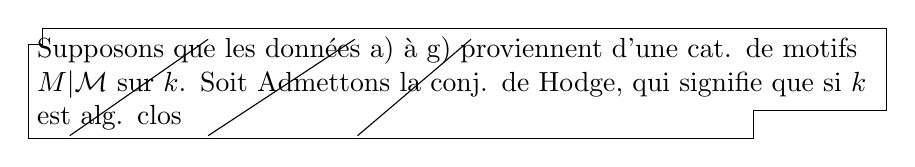
\begin{tikzpicture}[x=1cm,y=1cm]
\node[inner sep=3pt,text width=.88\linewidth,align=left] (oldblock) {\deleted{Supposons que les données a) à g) proviennent d'une cat. de motifs $\unsure{M|\mathcal M}$ sur $k$. \deleted{\unsure{Soit}} Admettons la conj. de Hodge, qui signifie que si $k$ est alg. clos}};
\draw ([xshift=5pt]oldblock.north west) -- (oldblock.north east) -- ([yshift=10pt]oldblock.south east) -- ([xshift=-48pt,yshift=10pt]oldblock.south east) -- ([xshift=-48pt]oldblock.south east) -- (oldblock.south west) -- ([yshift=-6pt]oldblock.north west) -- ([xshift=5pt,yshift=-6pt]oldblock.north west) -- cycle;
\draw ([xshift=15pt,yshift=1pt]oldblock.south west) -- ([xshift=65pt,yshift=-4pt]oldblock.north west);
\draw ([xshift=65pt,yshift=1pt]oldblock.south west) -- ([xshift=118pt,yshift=-4pt]oldblock.north west);
\draw ([xshift=119pt,yshift=1pt]oldblock.south west) -- ([xshift=160pt,yshift=-4pt]oldblock.north west);
\end{tikzpicture}}

Soit $V_{\mathbb Q},\ V_{\mathbb C}=\sum_{pq}V^{pq}$ une structure de Hodge, et soit $G$ son gpe de Mumford-Tate, donc $G_{\mathbb C}\subset\underline{\mathrm{Aut}}_{\mathbb C}(V)$. Soit $V_k\subsetV_{\mathbb C}$ une restriction des scalaires de $\mathbb C$ à $k\subset\mathbb C$, \deleted{\unsure{une}} \uline{compatible} avec la filtration naturelle de $V_{\mathbb C}$. Supposons que $(V_{\mathbb Q},\,V_{\mathbb C}=\sum V^{pq},\,V_k\subset V_{\mathbb C})$ provienne d'un motif sur \uuline{$k$}. \inserted{\deleted{Admettant}} \deleted{et admettons la conj. \unsure{de H.|de h}} \deleted{Alors}

Le gpe de Galois motivique de ce dernier, rel. à $T_{\mathrm{DR}}$, est \unsure{une|un} \deleted{forme} \inserted{groupe} $G'$ \unsure{déf}/$k$, \deleted{de $G_{\mathbb C}$,} et en vertu de \uline{conj. de Hodge} on doit avoir $G'_{\mathbb C}\unsure{=|\subset}G^\circ_{\mathbb C}$. \deleted{(\unsure{d'après} \illegible{2})} En d'autres termes, il faut que $G^\circ_{\mathbb C}$ soit ``définissable sur $k$ via $V_k\subset V_{\mathbb C}$'' ; c'est une condition très ; fort non triviale ! Lorsque $k$ est alg. clos, il faudra \deleted{\unsure{en}} $G'_{\mathbb C}=G_{\mathbb C}$, ce qu'on peut exprimer en disant que $\unsure{\forall|H}$ \deleted{invariant} élément d'un ${\bigotimes}_{\mathbb Q}^{\unsure{n|m}}(V'\otimes_{\mathbb Q}V)$ invariant sous $G$ (i.e. de bidegré $0$) est nécessairement dans $\bigotimes_{\unsure{k'|\bar k}}^{\unsure{n|m}}(V'_{\unsure{k'|\bar k}}\otimes_{\bar k}V_{\unsure{k'|K'}})$\unsure{!} ; si $k$ général, il faut \deleted{remplacer $k$ par une extension} \inserted{donc $\exists$ extension finie $k'$ de $k$,} ayant la vertu précédente. Ce sont encore des conditions très restrictives sur la structure envisagée. Elles ne sont certainement pas suffisantes (faire $k=\mathbb Q$, $V_k=V_{\mathbb Q}$, ce n'est en général pas possible
\figure{\begin{tikzpicture}[x=1pt,y=1pt]
\draw[dash pattern=on 8pt off 4pt] (0,0) -- (49,0);
\draw (55,6) -- (60,6) -- (61,0) -- (55,0);
\end{tikzpicture}}
% paper watermark, sideways, second fragment clipped at the lower edge
{\centering \textsc{\unsure{Strong}}\\
\textit{\unsure{uy|ny|y} \unsure{1808}}\par}
% archive sheet number: 30


\scanpage{32}
Il faut donc compléter les conditions \unsure{néc.|nèc.|nec.} \unsure{précédentes|précèdentes} par des \deleted{conjectures} \inserted{conditions} du type ``\unsure{arg.|conj.} de transcendance'',. pour éliminer le contre-exemple \unsure{précédent|précèdent|prècédent}.

% paper watermark, sideways
{\centering \textsc{Extra Strong}\\
\textit{\unsure{Ma}\unsure{in|nn}\unsure{ol|on}\unsure{uy|ny|y} 1808}\par}
% archive sheet number: 31


\scanpage{34}
\margin{\begin{tabular}{|l@{}}Situation abstraite du\\double réseau\\\hline\end{tabular}}
$\mathcal M$ $\otimes$-catégorie sur corps $k$,
\diagram{\begin{tikzcd}[ampersand replacement=\&,row sep=1pt,column sep=5pt]
{} \& L\arrow[dd,no head] \& {}\\
K\arrow[ur,no head]\arrow[dr,no head]\arrow[r,no head,shorten >=3pt] \& {} \& \deleted{\unsure{\neq|?}}\\
{} \& k \& {}
\end{tikzcd}}
diagramme de corps

\[
\begin{aligned}
T&\quad\text{foncteur fibre }/k\\
T'&\quad\rule{2.8cm}{.35pt}\quad K\quad\text{\deleted{extension de $k$}}\\
\varphi&\colon T\otimes_k L\simeq T'\otimes_K L\qquad\otimes\ \text{isom.}
\end{aligned}
\]

Soit
\[
\left\{\begin{aligned}
G&=\underline{\mathrm{Aut}}_{\otimes}(T)&\quad&\text{gpe affine sur }k\\
P&=\underline{\mathrm{Isom}}_{\otimes}(T_K,T')&&\text{torseur à droite sous }G_K\\
\varphi&\in P(L)
\end{aligned}\right.
\]
Ces données permettent de réconstituer $\mathcal M,T,T',\varphi$.

Supposons d'abord $P$ trivial, et soit $\unsure{\xi|\zeta}\in P(K)\subset P(\deleted{\unsure{K|k}}L)$. On a donc $\xi=\varphi g,\quad g\in G(L)$. Si on remplace $\xi$ par $\xi'$, on aura $\xi'=\xi a$, $a\in G(K)$, donc $g$ remplacé par $ga$. Donc on définit canoniquement
\[
\dot g\in G(L)/G(K),
\]
et on voit que la connaissance de $(G,\dot g)$ équivaut à celle de $(G,P,\varphi)$. Soit alors $V$ un $G$-module, alors le réseau $T'(V)\subset V\otimes_k L$ n'est autre que $g(V\otimes_k K)$. On a
\[
V\cap T'(V)=\{\,x\in V\}\mid g^{-1}x\in V\otimes_k K\,\}.
\]
\deleted{Soit $y=g^{-1}x$}

\unsure{S} \deleted{Donc Si \unsure{on} $k$ est un} Soit $\unsure{\gamma|y}$ l'image de $g$ dans $G_K$ (connue mod translations à droite par $a\in G(K)$), $\underset{\substack{\text{\unsure{l'adh.|adh.}}\\\text{\unsure{de|dans}}\ T_K}}{\overline{\{\gamma\}}}=T_K\subset G_K$, \inserted{Soit $y=g^{-1}x$ ;} alors \deleted{pour tt} comme \deleted{$\unsure{\gamma\,\mathrm{Tra}}$} $\gamma\in\mathrm{Transp}_{G_K}(x,y)(L)$, on a $T_K\subset\mathrm{Transp}_{G_K}(x,y)$, \deleted{pt $s$ de $T_K$ à valeurs ds une alg. sur $K$, \illegible{1}} donc pour deux \deleted{\unsure{tel}} \deleted{$s^{-1}x=\unsure{g|t}y$ donc si} $s,t$ \deleted{sont deux tels points on a} de $T_K$ (à val. dans une $K$-alg. quelc.) on a $s^{-1}a=t^{-1}x$ i.e. $ts^{-1}x=a$ i.e. $ts^{-1}\in(G_K)_x=(G_x)_K$.

Soit donc $R$ \unsure{:} l'adhérence de l'image de $T_k\times T_k\underset{\deleted{u}}{\longrightarrow}G_K$ par $(s,t)\unsure{\mathrel{-}|\longrightarrow}ts^{-1}$ ; il est immédiat qu'elle ne dépend pas du choix de $g$ mod $G(K)$, \deleted{et que}
\[
\boxed{R\subset G_K}
\]
% paper watermark, sideways, reversed on this face
{\centering \textsc{\unsure{Extra} \unsure{Strong}}\\
\textit{\unsure{Ma}\unsure{in|nn}\unsure{ol|on}\unsure{uy|ny|y} \unsure{1808}}\par}
% archive sheet number: 33


\scanpage{35}
l'on doit avoir, si $a\in V\cap T'(W)$, $R_K\subset G_{x\,K}$. L'inverse est vrai, car comme $T_K$ est fid. plat par $K$, on voit par descente que les pts (à coeff. ds des $K$-alg. quelconques $\Lambda$) $s.x$ $(s\in T_K(\Lambda))$ proviennent d'un pt bien déterminé de $V_K$. Or soit \deleted{\unsure{$\xi$}}
\[
S_K=\overline{\varphi(R_K)}\qquad p\colon G_K\unsure{\mathrel{-}|\longrightarrow}G,
\]
et soit $H$ le ss-gpe algébrique \inserted{fermé} de $G$ engendré par $S$. On a donc
\[
x\in V\cap T'(V)\quad\Longleftrightarrow\quad x\in V_{\deleted{\unsure{x|0}}}^{H}\quad \deleted{\unsure{H|\forall}\unsure{\subset|\in}\unsure{G}\ \unsure{H_x|H}\ \text{\unsure{tous|tels}}}.
\]

Par suite, pour que \deleted{les invariants} pour tout $V$, on ait $V\cap T'(V)=V^G$, i.e. que le foncteur $\mathrm{Rep}(G)=\mathcal M\longrightarrow$ (structures vectorielles mixtes pour $L(K/k)$ soit pl. fid, il f. et s. que pour $\forall\,V$, \deleted{les invariants} on ait
\[
V^H=V^G.
\]

Supposons $P$ quelconque. On a l'hom canonique de bitorseurs
\[
\deleted{\unsure{\underline{\mathrm{Isom}}|{\mathrm{Isom}}}_{\unsure{\otimes}}(\unsure{T'|T},T_K))}
\]
\diagram{\begin{tikzcd}[ampersand replacement=\&,row sep=small]
P\otimes_K P\arrow[r] \& G_K\\
(v,u)\arrow[r,mapsto] \& v^{-1}u
\end{tikzcd}}
\deleted{induisant}
\[
\deleted{P_L^G\times P_L\mathrel{-}G_L}
\]
donc $\varphi\colon\mathrm{Spec}\,L\longrightarrow P$ (un $\mathrm{Spec}\,K$-m., bien sûr) s'en déduit \deleted{de, grâce à l'isom $P_L\simeq G_L$}
\[
\mathrm{Spec}(L)\mathbin{\unsure{\otimes|\times}}_{\mathrm{Spec}\,K}\mathrm{Spec}(L)\mathrel{\unsure{-|\longrightarrow}}
P\mathbin{\unsure{\otimes|\times}}_{\mathrm{Spec}\,\unsure{K|k}}P\longrightarrow G_K\,;
\]
l'image fermée $\deleted{\unsure{P|R}}R_K$ est donc définie intrinsèquement. On vérifie encore (par descente \unsure{platisation|fidèlement|plate}) que \deleted{\unsure{p}} l'on a, pour tt $G$-module $V$
\[
\deleted{x\in}V\cap T'(V)=\{\,x\in V,\mid R_K\subset G_{x\,K}\,\}.
\]
Définissant $H$ comme ci-dessus, on trouve donc
\[
V\cap T'(W)=V^H,
\]
et la $\overline{\mathrm m}$ conclusion que plus haut ....
% paper watermark, sideways
{\centering \textsc{\unsure{Extra Strong}}\\
\textit{\unsure{Ma}\unsure{in|nn}\unsure{ol|on}\unsure{uy|ny|y} \unsure{1808}}\par}
% archive sheet number: 34


\scanpage{37}
% archive sheet number: 36
$K\subset\mathbb C$, $\bar K$ clôture alg. dans $\mathbb C$, $\pi_1=\pi_1(\mathrm{Spec}\,K,\bar K)=\mathrm{Gal}(\bar K/K)$, $\unsure{A|\mathcal A}={}$anneau des adèles ``finis'' de $\mathbb Q$. On \unsure{$^{1}$|$^{l}$}considère une catégorie de motifs sur $K$, de type fini, et le groupe de Galois \inserted{$G$} associé au foncteur de Betti. Cela donne naissance aux structures suivantes.

% Diagram across the head of the sheet; the small boxes share their frames' corners.
\diagram{\resizebox{\linewidth}{!}{\begin{tikzcd}[ampersand replacement=\&,column sep=4pt,row sep=7pt,execute at end picture={
 \draw ([xshift=-5pt,yshift=6pt]gd.north west) rectangle ([xshift=5pt,yshift=-8pt]gp.east |- gm.south);
 \node[draw,anchor=south east,inner sep=1pt] at ([xshift=5pt,yshift=-8pt]gp.east |- gm.south) {$D$};
 \draw ([xshift=-5pt,yshift=6pt]p.north west) rectangle ([xshift=5pt,yshift=-12pt]g.south east);
 \node[draw,anchor=south east,inner sep=1pt] at ([xshift=5pt,yshift=-12pt]g.south east) {$B$};
 \draw (p.south) -- (avec.north);
 \draw (conn.center) ellipse [x radius=38pt,y radius=13pt];
 \draw (pc.south) -- (ptc.north);
 \draw (qc.south) -- (ptq.north);
 \draw (ptc.center) ellipse [x radius=37pt,y radius=14pt];
 \node[draw,anchor=south east,inner sep=1pt] at ([xshift=5pt,yshift=-3pt]ptc.south east) {$C$};
 \node[draw,anchor=south east,inner sep=1pt] at (ga.south east) {$A$};
}]
 |[alias=gd]| G''_K \arrow[r,phantom,"{\supset}" description] \& H''_K\arrow[r,dash,dashed] \& Q\arrow[r,dash,dashed] \& H'_K \&[-4pt] {\subset} \&[-4pt] |[alias=gp]| G'_K\arrow[r,dash,dashed] \& |[alias=p]| P\arrow[r,dash,dashed] \& |[alias=g]| G_K \&[13pt] |[alias=pc]| P_{\mathbb C} \& G_{\mathbb C} \& |[alias=qc]| Q_{\mathbb C} \&[8pt] |[draw,alias=ga,minimum width=34pt,minimum height=24pt]| G\\
 |[alias=gm]| \mathbb G_m\arrow[u,shift left=1,"i_1"]\arrow[u,shift right=1,"i_2"'] \& \& \& \& \& \& |[alias=avec]| \text{avec} \& \& |[alias=ptc]| \begin{gathered}\text{avec pt }\deleted{\unsure{\xi|a}}\ \alpha\\\text{rat}/\mathbb C,\ \text{de}\end{gathered} \& \& |[alias=ptq]| \begin{gathered}\text{avec pt }\unsure{\xi_1|\alpha_1}\\\text{rat}/\mathbb C,\end{gathered} \& \\
 \& \& \& \& \& \& |[alias=conn]| \begin{gathered}\text{connexion absolue}\\\text{intégrable}\end{gathered} \& \& \text{sorte que} \& \& \& \\
 \& \& \& \& \& \& \begin{gathered}\text{invariante}\\\text{par }G_K\\{}[\,\text{NB structure vide}\\\text{si }K\ \text{abst. alg}\,]\end{gathered} \& \& \& \& \&
\end{tikzcd}}}

\diagram{\begin{tikzcd}[ampersand replacement=\&,column sep=25pt,execute at end picture={\draw ([xshift=-3pt,yshift=6pt]pu.north west) rectangle ([xshift=4pt,yshift=-4pt]gu.south east); \node[draw,anchor=south east,inner sep=1pt] at ([xshift=4pt,yshift=-4pt]gu.south east) {$G$};}]
 |[alias=pu]| \pi_1 \arrow[r,"{\substack{\deleted{\unsure{v|w}}\\u}}"] \& |[alias=gu]| G(A)
\end{tikzcd}}
\[
 \deleted{(\pi_1)_{\mathbb Q}\xrightarrow{\unsure{v|u}}G/G^\circ\quad\text{i.e.}\quad\pi_1\to(G/G^\circ)(\mathbb Q)}
\]

\uline{NB} La donnée \deleted{\unsure{principale}} compliquée $\boxed D$ peut être remplacée par la ``donnée subordonnée'' $\boxed E$, \uline{soumise} à la condition d'être ``compatible'' avec $A,B,C$

a) la connexion absolue définit
\[
 \omega\in\Omega^1_{\mathbb C/\mathbb Q}\otimes_{\mathbb Q}{\mathfrak g}_{\mathbb Q}
\]

b)
\diagram{\begin{tikzcd}[ampersand replacement=\&,column sep=0pt,row sep=0pt]
 G' \& \otimes_K\mathbb C \&[5pt] \simeq \&[5pt] G_{\mathbb C}\\
 {\rotatebox{90}{$\subset$}} \& \& \&\\
 H' \& \otimes_K\mathbb C \& \&\\
 {\rotatebox{90}{$\simeq$}} \& \& \&\\
 H'' \& \otimes_K\mathbb C \& \&\\
 {\rotatebox{90}{$\simeq$}} \& \& \&\\
 G''_1 \& \otimes_K\mathbb C \& \simeq \& G_{\mathbb C}
\end{tikzcd}}

c) d'où des hom
\diagram{\begin{tikzcd}[ampersand replacement=\&,row sep=1pt,column sep=8pt]
 \& \& \boxed E\arrow[d]\\
 i_1^{\mathbb C},\nu_2^{\mathbb C}:G_{m\,\mathbb C}\arrow[r] \& G_{\mathbb C} \& {}
\end{tikzcd}}

d) On a, pour un modèle régulier convenable $S$ de $K$, de type fini sur $\mathbb Z$ (supposons $K$ de t.f. sur $\mathbb Q$)
\diagram{\begin{tikzcd}[ampersand replacement=\&,column sep=16pt,row sep=5pt,execute at end picture={\draw ([xshift=-4pt]ds.south east) |- ([xshift=2pt,yshift=2pt]geom.north);}]
 \& \& \boxed G\\
 |[alias=ds]| \pi_1(S(\mathbb C),{\unsure{\xi|\zeta}})\arrow[r,"w"] \& G(\mathbb C). \&\\
 |[alias=geom]| \begin{gathered}\text{pt géom}\\\text{déduit de}\\\text{l'inclusion}\\K\subset\mathbb C\end{gathered} \& \begin{gathered}{}[\,\text{NB : structure}\\\text{vide si }K\text{ est}\\\text{abst. alg.}\,]\end{gathered}\&
\end{tikzcd}}

% The line running from e) meets the lower right corner of the boxed consequence.
\diagram{\resizebox{\linewidth}{!}{\begin{tikzcd}[ampersand replacement=\&,column sep=9pt,row sep=5pt,execute at end picture={
 \coordinate (cl) at ([xshift=-4pt]lh.west);
 \coordinate (cr) at ([xshift=6pt]qr.east);
 \draw ([yshift=3pt]cl |- lh.north) rectangle ([yshift=-4pt]cr |- lb.south);
 \draw ([xshift=-13pt,yshift=-9pt]lh.west) circle [radius=2pt];
 \draw ([xshift=-13pt,yshift=-9pt]lh.west) -- ([xshift=1pt,yshift=5pt]lh.north west);
 \draw[rounded corners=6pt] ([xshift=-8pt,yshift=1pt]eb.south west) -- ([xshift=-4pt,yshift=-4pt]cr |- lb.south) -- ([xshift=-6pt,yshift=6pt]et.north west) -- ([xshift=8pt,yshift=4pt]et.north east) -- ([xshift=10pt,yshift=-1pt]eb.south east) -- ([xshift=-8pt,yshift=-2pt]eb.south west) -- cycle;
}]
 |[alias=lh]| \text{Il en résulte aussi que le diagramme} \& {} \&[25pt] {}\\
 \pi_1(S(\mathbb C),\xi)\arrow[r,"{\unsure{w|{}}}"]\arrow[d,"\mathrm{can.}"] \& |[alias=qr]| G(\mathbb Q)\arrow[d] \& |[alias=et]| \begin{gathered}\text{e) }P/G^\circ\text{ est un}\\\text{torseur sur }K,\ \text{de}\end{gathered}\\
 \pi_1(S,\xi)\arrow[r,"v"] \& G/G^\circ(\mathbb Q) \& \begin{gathered}\text{groupe }G/G^\circ,\ \text{ponctué}\\\text{par }\xi:K\to\mathbb C,\ \text{donc}\end{gathered}\\
 |[alias=lb]| \text{est commutatif} \& {} \& |[alias=eb]| \begin{gathered}\text{définit}\quad v:\pi_1\longrightarrow(G/G^\circ)(\mathbb Q)\\\text{i.e.}\quad\pi_1\longrightarrow(G/G^\circ)_{\mathbb Q}\end{gathered}
\end{tikzcd}}}

\uline{Propriétés}

1) $i_2^{\mathbb C}=\overline{i_1^{\mathbb C}}$ (donc $\unsure{\alpha_1|\alpha}$ est connu quand on connaît $\alpha$)

2) $\pi_1(S(\mathbb C),\xi)\to G(\mathbb C)$ se factorise par $G(\mathbb Q)$, \deleted{et on a \unsure{compatibilité}}

3) $\pi_1\to G(A)$ se factorise par $\pi_1(S,\xi)\unsure{\mathrel{-}|\to}G(A)$ pour $S$ convenable

4) les diagr.
\diagram{\begin{tikzcd}[ampersand replacement=\&,column sep=27pt]
 \pi_1(\deleted{\unsure{S|C}}S(\mathbb C)\deleted{\unsure{,\xi|)}} ,\xi)\arrow[r,"{\deleted{\unsure{\pi_1|u}}}","w"']\arrow[d,"\mathrm{can.}"] \& G(\mathbb Q)\arrow[d,"\mathrm{can.}"]\\
 \pi_1(S,\xi)\arrow[r,"u"] \& G(A)
\end{tikzcd}\hspace{5pt}\begin{tikzcd}[ampersand replacement=\&,column sep=13pt]
 \pi_1\arrow[r,"v"]\arrow[d,"u"] \& G/\deleted{\unsure{G'|G}}G^\circ(\mathbb Q)\arrow[d]\\
 \deleted{\unsure{u|G}}G(A)\arrow[r] \& (G/G^\circ)(A)
\end{tikzcd}}
\unsure{sont|\deleted{sont}} commutatifs. \unsure{!|/}

5) Le composé $\pi_1(S,\xi)\mathrel{-}G(A)\xrightarrow{\varepsilon}A^*$ est l'hom défini par l'action de $\pi_1(S,\xi)$ sur les racines de l'unité.

% This addition occupies the lower right of the sheet. Its linking stroke begins after 5).
\figure{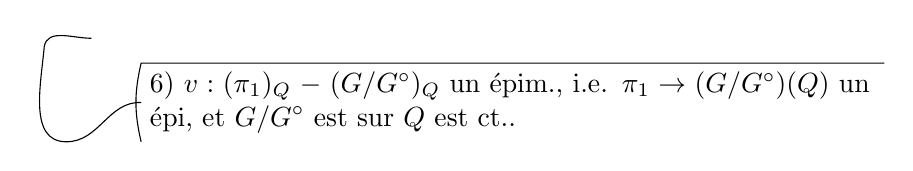
\begin{tikzpicture}
 \node[inner sep=3pt,text width=.76\linewidth,align=left] (addsix)
 {\inserted{6) $v:(\pi_1)_{\mathbb Q}\mathrel{-}(G/G^\circ)_{\mathbb Q}$ un épim., i.e. $\pi_1\to(G/G^\circ)(\mathbb Q)$ un épi, et $G/G^\circ$ \deleted{\unsure{est}} sur $\mathbb Q$ est \uuline{ct.}.}};
 \draw (addsix.north east) -- (addsix.north west) to[bend right=13] (addsix.south west);
 \draw (addsix.west) to[out=178,in=0] ([xshift=-27pt]addsix.south west) to[out=180,in=-95] ([xshift=-35pt,yshift=6pt]addsix.north west) to[out=80,in=180] ([xshift=-18pt,yshift=9pt]addsix.north west);
\end{tikzpicture}}

\deleted{\unsure{6|7}}7) Pour tout point fermé $s$ de $S$, l'élément de \unsure{frobénius|frobènius} $f_s$ de $\pi_1(S,\xi)$ a \deleted{comme image} \inserted{une} classe dans $G(A)$ \inserted{qui correspond à} l'image d'une classe de conjugaison de $G\deleted{\unsure{(A)|_{\mathbb Q}}}$ (redonne Weil \unsure{...|....}).

% slanted
\margin{devra être \unsure{précisé|precisé} ...}

\deleted{\unsure{7|8}}8) $G_{\mathbb R}$ muni de $i_1^{\mathbb C},i_2^{\mathbb C}$ de c) est un \uline{groupe de Hodge}.

\deleted{\unsure{8|9}}9) (Modulo Tate) Pour tout $\unsure{l|\ell}$, l'image de $\pi_1\unsure{k|K|\xi}$ dans $G(\mathbb Q_l)$ est un sous-groupe opérant de façon $\frac12$ simple sur tout \deleted{\unsure{produit|foncteur|générateur}} $V\otimes_{\mathbb Q}\mathbb Q_l$ \deleted{\unsure{engendre|engendré} $\mathbb Q_l$ comme}, (ou \uline{un} tel, avec $\deleted{\unsure{V|D}}V$ \deleted{seul} fidèle), et son enveloppe algébrique est $G_{\mathbb Q_l}$.

\deleted{\unsure{Le composé} $\pi_1\to G(A)\to G(\mathbb Q_l)\unsure{\mathrel{-}|\to}G/G^\circ$}

% paper watermark, sideways
{\centering \textsc{\unsure{Extra} \unsure{Strong}}\\
\textit{\unsure{Ma}\unsure{in|nn}\unsure{ol|on}\unsure{uy|ny|y} \unsure{1808}}\par}


\scanpage{38}
% The writing is turned 180 degrees in the scan.
\[
\begin{aligned}
G'_{K} \quad P \qquad G_{K} &\qquad G_{\mathbb{C}} / \mathbb{C} \\
                            &\qquad G / \mathbb{Q}
\end{aligned}
\]

\unsure{,|1|)}

% Paper watermark, sideways and mirrored relative to the manuscript; two lines.
\noindent\textsc{Extra Strong}\\
\unsure{Maunoury|Marmury|Maimury} 1808
% archive sheet number: 37


\scanpage{39}
Nous allons introduire une autre structure de nature transcendante, en introduisant le rev. universel $\bar S_{\mathbb C}$ de $S(\mathbb C)$ en $\xi$ $\xi$ [sous-entendu : de la comp. connexe de $\xi$ dans $S(\mathbb C)$].

Soit $\unsure{\gamma|\mathscr{Y}}_{G}$ l'ensemble des hom. de $\mathbb S=\prod_{\mathbb C/\mathbb R}\mathbb G_{m\,\mathbb C}$ dans $G_{\mathbb R}$, correspondant à l'hom central \deleted{donné} $i:\mathbb G_m \relbar G$ donné par $i(\lambda)=i_1(\lambda)i_2(\lambda)$. \margin{\rule{0.35pt}{2.1\baselineskip}}On considère $\gamma$ comme variété \deleted{\unsure{an.|anal.}} holomorphe où \deleted{$\unsure{\gamma|G}$} $G(\mathbb R)$ et à fortiori $G(\mathbb Q)$ opère. Ceci posé, on a une \uline{application}
\[
\boxed{f:\bar S_{\mathbb C}\longrightarrow\gamma_G}
\]
satisfaisant les conditions

\uline{12)}a. \ a) $f(\bar\xi\inserted{\text{le pt marqué de }\bar S_{\mathbb C}})={}\text{l'hom }\mathbb S\relbar G_{\mathbb R}$ défini par $i_1^{\mathbb C},i_2^{\mathbb C}$ de c).

b) $f(g\bar s)=\unsure{w_{1}|w}(g)f(\bar s)$ si $g\in\pi_1(S(\mathbb C),\xi),\ \bar s\in\bar S_{\mathbb C}$

c) $f$ est \uline{holomorphe}.

\unsure{14)|15)} (Moyennant Hodge) \deleted{Pour tout $\bar s\in\bar S_{\mathbb C}$, le plus grand sous-groupe algébrique de $G$ qui sur $\mathbb R$ contient $f(\bar s)(\mathbb S)\subset G_{\mathbb R}$, et qui de plus contient $H$} \inserted{Le composé \deleted{\unsure{de}} $\bar S_{\mathbb C}\longrightarrow\gamma_G\longrightarrow\gamma_{\widetilde G}$} (qui à priori \inserted{\unsure{vû|vu|n\textsuperscript{o}} : 12 b)} se factorise par \deleted{\unsure{$\bar S_{\mathbb C}$}} $S(\mathbb C)^{\circ}$) est une application \uline{constante}.

13) Si $\bar s\in\bar S_{\mathbb C}$ se trouve sur le point $t$ de $S$ [il nous \unsure{plait|plaît} bien que $P$ comme torseur à connexion \unsure{intég.|intégr.} $P_S$ soit défini sur $S$] de sorte qu'on a torseur à conn. intégrable \deleted{\illegible{1}} $(P_t,G_{k(t)})$ sur $k(t)$, \deleted{\unsure{soit}} l'hom $f(\bar s)_{\mathbb C}:\mathbb S_{\mathbb C}\longrightarrow(G_{k(t)})_{\mathbb C}\simeq G_{\mathbb C}$ [définissant une bigraduation\inserted{ (donc filtration)} sur le foncteur $T_{\mathbb C}$, $T$ foncteur oubli sur les $G$-modules] est \uline{compatible} avec le torseur $P_t$ sous $G_{k(t)}$ et sa $C$-trivialisation $p(\bar s)$ [$p:\bar S_{\mathbb C}\longrightarrow(P_S)_{\mathbb C}$ $\unsure{\in|\epsilon}$ \unsure{ici est|est} la $S(\mathbb C)^{\circ}$-morphisme caractérisé par la condition que $p(\bar\xi)=\alpha$].
% archive sheet number: 38


\scanpage{40}
\unsure{10)|19)} (Modulo conjecture de Hodge) $G^{\circ}$ est engendré sur $\unsure{\mathbb Q|Q}$ par $i_1^{\mathbb C}$.

\deleted{\unsure{10)} $G$}

% slanted
\margin{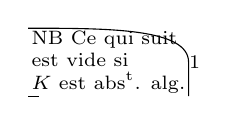
\begin{tikzpicture}[baseline=(current bounding box.north),font=\scriptsize]
\node[align=left,inner sep=1pt] (note) {\uline{NB} Ce qui suit\\est vide si\\$K$ est abs\textsuperscript{t}. alg.};
\draw (note.north west) .. controls (note.north) and (note.north east) .. (note.east)
.. controls (note.east) and (note.south east) .. (note.south east);
\draw (note.south west) -- ([xshift=4pt]note.south west);
\node[anchor=west,inner sep=0pt] at (note.east) {\deleted{\illegible{1}}};
\end{tikzpicture}}
Soit $R\subset G$ le sous groupe algébrique engendré par $w(\pi_1(S(\mathbb C),\xi))$. Il est \uline{invariant} moyennant \unsure{9)|4)} [car l'image fermée de $\pi_1(S(\mathbb C),\unsure{\xi|1})\relbar\pi_1(S,\xi)$\} est un sous-groupe invariant\}, le quotient étant $\pi_1(\operatorname{Spec} k,\xi)$, où $k$ est la clôture alg. de $\mathbb Q$ dans $K$]. \deleted{Le \unsure{composé}} En vertu de 4), l'hom.
\diagram{\begin{tikzcd}[ampersand replacement=\&,column sep=1.4em,row sep=.5ex]
{} \& {} \& \inserted{\widetilde G(\mathcal A),\ \text{où }\widetilde G=G/R,}\\
\pi_1(S\unsure{\mathbb C|\in},\xi) \arrow[r] \& G(\unsure{\mathcal A|\mathscr A|A}) \arrow[ur] \& {}
\end{tikzcd}}
se factorise donc en
\[
\tilde u:\underset{\substack{\Vert\\[-.4ex]\simeq\\[-.4ex]\unsure{\pi_1|\Vert}}}{\pi_1(\operatorname{Spec}(k),\xi)}
\longrightarrow\widetilde G(\mathcal A)
\]

D'autre part, on considère le torseur $\widetilde P=P/R$ sous $\widetilde G$, avec la connexion intégrable déduite de celle de $P$. On a

\margin{\deleted{\uline{\illegible{1}}}}
\unsure{16)|18)|10)} \inserted{(Modulo Hodge)} $(\widetilde P,\widetilde G)$ avec sa connexion intégrable ``se descend à $k$'', donc on a un torseur $(\widetilde P_0,(\widetilde G/k)$ sur $k$, et un isom de torseurs
\begingroup
\csname tagsleft@true\endcsname
\[
\widetilde P=P/R\simeq\widetilde P_0\otimes_k K \tag*{(*)}
\]
\endgroup

\deleted{De plus, \deleted{posant} introduisant $R'\subset G'$ correspondant à $R$, et $\widetilde G'=G'/R'$, de sorte qu'on a un isom}
\[
\deleted{\widetilde G'=\widetilde G'_0\otimes_k K,\qquad
\widetilde G'_0=\underline{\operatorname{Aut}}_{(\widetilde G/k)-}(\widetilde P_0),}
\]
\deleted{le ss-groupe \deleted{$\unsure{\widetilde H'|H'}\subset\unsure{\widetilde G'|G'}$} \inserted{$\widetilde H'=H'/H'\cap R'\unsure{=|\simeq}\operatorname{Im}(H'\longrightarrow\widetilde G')$} est ``défini sur $k$'' i.e. provient de $\widetilde H'_0\subset\widetilde G'_0$}

\inserted{Enfin l'isom \unsure{(*)|ci}, $\unsure{\in|\xi}$ qui} \deleted{La structure de filtration sur le foncteur $T$} définit, pour un $\widetilde G$-module $M$, une structure de descente sur $P\mathbin{\times}^{G_K}M_K$ à $k$\unsure{,|;} [c'est celle définie par la connexion intégrable de $P\mathbin{\alpha}^{G_K}M_K$], donne une donnée de descente \uline{compatible} avec la filtration, i.e cette dernière est \uline{horizontale}, $\bigl[\!\bigl[$ donc \deleted{\illegible{1}} $\widetilde H'=\operatorname{Im}(H'\longrightarrow\widetilde G')$, $\widetilde Q,=Q\mathbin{\times}^{\unsure{H'|\widetilde H'}}\widetilde H'$, se descendent \unsure{respect\textsuperscript{t}|respectiv\textsuperscript{t}} en $\widetilde H'_0\subset\widetilde G'$ et un torseur à droite $Q_0$ sous $\widetilde H'_0$, \unsure{\deleted{et}|et} (d'où $\widetilde H''_0$ et $\widetilde G''_0$ qui descendent $H''$ et $\widetilde G''$), et \deleted{\unsure{après}} les composés $\tilde i_1,\tilde i_2:\mathbb G_m\underset K{\relbar}G''\longrightarrow\widetilde G''$ se descendent en $(\tilde i_1)_0,(\tilde i_2)_0:\mathbb G_{m\,k}\longrightarrow\widetilde G''_0$ $\bigr]\!\bigr]$.
% archive sheet number: 39


\scanpage{41}
$S$ schéma régulier connexe de \unsure{t.f.|v.f.} sur $\unsure{\mathbb Q|Q}$

$k$ clôture alg. de $\mathbb Q$ dans $\Gamma(S,\unsure{\mathscr O|\mathcal O}_S)$, de sorte que $k/\mathbb Q$ fini, $S/k$ géom. \unsure{conn|conn.}

$k\hookrightarrow\mathbb C$ une immersion

$\mathcal M$ catégorie de motifs (``iso'', lisses $\frac12$ simples) sur $S$, $\mathcal M$ de type fini.

L'immersion $k\hookrightarrow\mathbb C$ définit une classe d'isomorphie de foncteurs fibres\inserted{ val\,/\,$\mathbb Q$} sur $\mathcal M$, savoir les $T_{\xi}\deleted{\unsure{T|P}}:M\longrightarrow T_B(M_{\xi}),\quad \xi\in S(\mathbb C)$\inserted{$\underset{\deleted{\operatorname{Hom}_k(\operatorname{Spec}\mathbb C,S)}}{\Vert}$}.

Soit \deleted{$G$ un groupe alg. /$\mathbb Q$ (réductif) isomorphe aux $\underline{\operatorname{Aut}}_{\otimes}(T_{\xi})$\unsure{en|.}.} \inserted{$T$ un foncteur fibre de cette classe, et \deleted{\unsure{soit}}}
\[
G=\underline{\operatorname{Aut}}_{\otimes}(T),\quad\text{donc }\mathcal M\approxeq\operatorname{Rep}(G)
\]

Alors
\[
P=\underline{\operatorname{Isom}}_{\otimes}(T_S,T_{\mathrm{DR}})
\]
est un torseur sous $G_S$. Il est muni d'une \uline{connexion} intégrable relativement à $k$ (ou $\mathbb Q$, c'est kif kif) compatible avec $G$,

De plus le foncteur $T_{\mathrm{DR}}$, isomorphe par construction de $P$ à
\[
M\longmapsto P\mathbin{\times}^{G_S}M_S\qquad\text{sur }\operatorname{Rep}(G)
\]
est muni d'une $\otimes$-\uline{filtration}

\deleted{Soit $S_{\mathbb C}$} Considérons $S(\mathbb C)$, et le revêtement $\deleted{\bar S}\unsure{\widetilde P|\bar P}_{\mathbb C}$ de $S(\mathbb C)$ dont la fibre en $\xi\in S(\mathbb C)$ est formée des isom $T\longrightarrow T_{\xi}$. Alors $\bar S_{\mathbb C}$ est un revêtement principal de $S(\mathbb C)$, de groupe $G(\mathbb Q)$, \deleted{qui n'est autre que le rev. \unsure{associé}, \unsure{fibré} \unsure{pr.} assoc. à $P_{\mathbb C}^{\mathrm{an}}$ sur $S_{\mathbb C}^{\mathrm{an}}\underset{S(\mathbb C)}{\Vert}$} et \unsure{un|on} \deleted{\unsure{une}} \deleted{\unsure{avec|de} $S_{\mathbb C}$} \deleted{\unsure{application}} \inserted{morphisme (hol)} évident
\[
p:\deleted{\unsure{\bar S|\bar P}}\widetilde P_{\mathbb C}
\longrightarrow P_{\mathbb C}^{\mathrm{an}}\deleted{\unsure{G|g}}
\]
satisfaisant
\[
\left[\begin{aligned}
&p(\unsure{\xi|g}\,\times\,g)=p(x)g\\
&p\ \text{compatible aux connexions \unsure{sur un|sur nos|sur}}\\
&\hspace{4em}S\text{-fibrés}\ldots
\end{aligned}\right.
\]

\[
\deleted{f:\bar S_{\mathbb C}\longrightarrow\unsure{\gamma|\mathscr Y}_{G}}
\]
\deleted{où $\gamma_G$ est l'espace des structures de Hodge sur $G_{\mathbb R}$ (compatibles, si on y tient, avec un $i:\mathbb G_m\relbar G$ fixé). Alors $f$ satisfait aux conditions}

\deleted{a) $f$ holomorphe}

\deleted{b) $f(xg)=g^{-1}f(x)$ pour $g\in G(\mathbb Q)$ [\uline{NB} $G(\mathbb R)$ donc $G(\mathbb Q)$ opère sur $\gamma_G$ par autom. \unsure{intérieurs|intégrieurs},]}

\deleted{c) .}
% archive sheet number: 40


\scanpage{42}
Lorsqu'on se fixe un point $\xi_0\in S(\mathbb{C})$,\deleted{\unsure{$\xi$|,}}\inserted{et qu'on prend $T=T_{\xi_0}$,} alors la donnée du revêtement principal $\bar S_{\mathbb{C}}$ et de $\deleted{\unsure{f|p}}p$ équivaut à la donnée de
\[
\begin{aligned}
&\deleted{\unsure{w(\pi_1(S(\mathbb{C}),\xi_0)|w:\pi_1(S(\mathbb{C}),\xi_0)}}\\
&\unsure{w|\omega}:\pi_1(S(\mathbb{C}),\xi_0)\longrightarrow G(\mathbb{Q})\subset G(\mathbb{C})
\end{aligned}
\]
[il est associé à la connexion intégrable de $P$, qui en définit une sur $P_{\mathbb{C}}^{\mathrm{an}}$ sur $S_{\mathbb{C}}^{\mathrm{an}}$, d'où $\Gamma=\pi_1(S(\mathbb{C}),\xi_0)\longrightarrow G(\mathbb{C})$, dont il faut demander qu'il se factorise par $G(\mathbb{Q})$] et à un \deleted{hom du revêtement universel} point $\alpha_0$ de $P(\xi_0)$ i.e. une trivialisation de $P_{\xi_0}$, qui définit alors un unique morphisme \inserted{$q$} du rev. universel $\bar S_{\mathbb{C}}$ de $S_{\mathbb{C}}$ dans $P_{\mathbb{C}}^{\mathrm{an}}=P(\mathbb{C})$, appliquant le pt marqué $\bar\xi_0$ en $\alpha_0$ ; il satisfait \deleted{\unsure{à|la}} $q(\bar s\gamma)=q(\bar s)\unsure{w|W}(\gamma)$ pour tout $\hat s\in\bar S_{\mathbb{C}}$, \deleted{$\unsure{\gamma\in\pi_1(S|\gamma\in\pi_1}$} $\gamma\in\Pi_1(S(\mathbb{C}),\xi_0)$, \deleted{Le morphisme \unsure{satisfai|satisfait}} et définit
\[
\widetilde P_{\mathbb{C}}=\overline{\unsure{S|\mathbb{S}}}_{\mathbb{C}}\mathbin{\times}^{\Gamma}G(\mathbb{Q})\hookrightarrow P_{\mathbb{C}}^{\mathrm{an}}
\]
[\unsure{restriction|restiction} du groupe structural \inserted{du $P_{\mathbb{C}}^{\mathrm{an}}$} de $G(\mathbb{C})$ à $G(\mathbb{Q})$].

Comme structure importante, il y a une application
\[
f:\widetilde P_{\mathbb{C}}\longrightarrow\unsure{\gamma|\mathscr{Y}}_G
\]
où $\gamma_G$ est l'ens. des structures de Hodge sur $G_{\mathbb{R}}$ (\deleted{associées,}\inserted{compatibles,} si on y tient, avec un morphisme $i:\mathbb{G}_{m\,\mathbb{Q}}\longrightarrowG$ donné). Cette application $f$ satisfait les conditions

a) $f$ holomorphe

b) $f(xg)=g^{-1}f(x)$ \qquad $g\in G(\mathbb{Q}),\,x\in\widetilde P_{\mathbb{C}}$

\unsure{b|c}) $\forall x\in\widetilde P_{\mathbb{C}}$ sur le point $s$ de $S$, la \inserted{structure de} filtration sur $T_{\mathbb{C}}$ sur $\operatorname{Rep}(\unsure{G|C})$, définie par $f(\unsure{x|s}):\mathbb{S}\longrightarrow G_{\mathbb{R}}$, est compatible
% archive sheet number: 41


\scanpage{43}
avec le torseur $P_s$ sous $G_{k(s)}$ et la trivialisation $p(x)\in P_s(\mathbb{C})$.

En termes de $\unsure{w|\omega}$ et $q:\bar S_{\mathbb{C}}\longrightarrow P_{\mathbb{C}}^{\mathrm{an}}$, la donnée de $f$ revient à la donnée de
\[
f:\bar S_{\mathbb{C}}\longrightarrow\unsure{\gamma|\mathscr{Y}}_G
\]
satisfaisant les conditions

a) $f$ holomorphe

b) $f(xg)=w(g)^{-1}f(x)$

c) \deleted{$\unsure{f(\xi_0)|f(\bar\xi_0)}$} $\forall\bar s\in\bar S_{\mathbb{C}}$, \inserted{sur $s\in S$} $f(\bar s):\mathbb{S}\relbarG_{\mathbb{R}}$ est compatible avec le torseur $P_s$ sur $G_{k(s)}$ et sa trivialisation $q(x)\in P_s(\mathbb{C})$.

Enfin, \deleted{pour tout $k$}, on se donne une ``\unsure{restiction|restriction}'' du rev. $\widetilde{\mathbb P}_{\mathbb{C}}\mathbin{\times}^{G(\mathbb{Q})}G(\mathcal A)\deleted{\mathbb{Q}_{\ell}}$ sur $S_{\mathbb{C}}^{\mathrm{an}}$ en un revêtement
% slanted
\margin{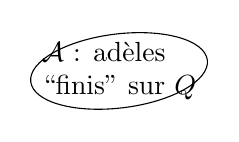
\begin{tikzpicture}[baseline=(current bounding box.center)]
\node[inner sep=0pt,align=left] (note) {$\mathcal A$ : adèles\\``finis'' sur $\mathbb{Q}$};
\draw[rotate around={7:(note.center)}] (note.center) ellipse [x radius=1.13cm,y radius=.47cm];
\end{tikzpicture}}
\deleted{sur $S$ dont de \unsure{gpe|grp} $G_\ell$} de groupe $G(\mathbb{Q}_{\ell})$ sur $S$, En termes \inserted{de $\xi_0$ et} de $\Gamma=\pi_1(S(\mathbb{C}),\unsure{\xi|\mathord{)}}_0)$, on se donne une factorisation de $\Gamma\xrightarrow{w}G(\mathbb{Q})\relbarG(\mathcal A)$ par $\Gamma\longrightarrow\Pi_1\underset{\substack{\Vert\\\Pi_1}}{(S},\xi_0)\longrightarrow G(\mathcal A)$. Quant au revêtement $\widetilde P_{\mathbb{C}}\mathbin{\times}^{G(\mathbb{Q})}(\deleted{\unsure{G|\mathcal A}}\mathcal A/G^{\unsure{0|\circ}})(\mathcal A)$, \deleted{égal à $\widetilde P_{\mathbb{C}}\times$}\inserted{il est} associé à $\widetilde P_{\mathbb{C}}/G^0(\mathbb{Q})\deleted{\text{de}}\unsure{=|\relbar}(P/G^0)_{\mathbb{C}}^{\mathrm{an}}$, \deleted{\unsure{qui|qu'}}et \unsure{à|:} ce titre \unsure{leur|leurs} restriction à $S$ \deleted{\unsure{est|et}} est connue. On veut que ce sont celles données plus haut.....

\deleted{\uline{NB} \unsure{L'application|l'application} $f$ \unsure{est|et}}
% archive sheet number: 42


\scanpage{44}
A) Groupe algébrique \deleted{\unsure{$G$|$E$}}\unsure{[|(}réductif] $G$ sur $\mathbb{Q}$

B) fibre principal à connexion intégrable $\unsure{P|\mathbb P}$ sur $G_S$

% slanted; marginal brace extends alongside C) and D)
\margin{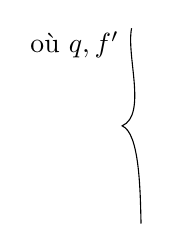
\begin{tikzpicture}[x=1cm,y=1cm,baseline=(current bounding box.north)]
\node[anchor=north east,inner sep=1pt] at (-.09,0) {où $q,f'$};
\draw (.03,0) .. controls (-.04,-.35) and (.23,-1.10) .. (-.09,-1.24)
.. controls (.13,-1.33) and (.14,-2.05) .. (.15,-2.48);
\end{tikzpicture}}
C) Restriction du groupe $G_{\mathbb{C}}^{\mathrm{an}}$ à $G(\mathbb{Q})$ dans $P_{\mathbb{C}}^{\mathrm{an}}$, d'où
\diagram{\begin{tikzcd}[ampersand replacement=\&,column sep=2em]
\text{rev.}\quad\deleted{\unsure{\bar S|\widetilde S}}\quad\widetilde P \arrow[r,hook,"p"] \& P_{\mathbb{C}}^{\mathrm{an}} \arrow[r] \& P
\end{tikzcd}}

D) Application holomorphe
\[
f:\widetilde P\longrightarrow\unsure{\gamma|\mathscr{Y}}_G
\]
satisfaisant $f(xg)=g^{-1}f(x)$ $(x\in\widetilde P,\,g\in G(\mathbb{Q})$ et compatible avec les données B) et $p$ de C).

E) Restriction de $\widetilde P\mathbin{\times}^{G(\mathbb{Q})}G(\mathcal A)$ à $S$, avec compatibilité relativement à $G/G^{\circ}$.

NB La connaissance de A) B) C) et de $f(\xi_0)$, où $\xi_0\in\widetilde P$ est au dessus du point générique de $S$ [\uline{Condition} peut-\uline{être superflue}] \margin{??}doit en principe permettre de réconstituer D) tout entier et E) [lorsqu'on sait \deleted{que} que les données proviennent d'une cat. de motifs $M$].

% slanted; boxed marginal note
\margin{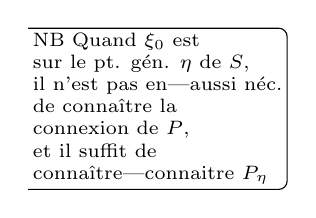
\begin{tikzpicture}[baseline=(current bounding box.north)]
\node[align=left,inner sep=1.5pt,font=\scriptsize] (note) {\uline{NB} Quand $\xi_0$ est\\
sur le pt. gén. $\eta$ de $S$,\\
il n'est pas \deleted{\unsure{en|aussi}} néc.\\
de connaître la\\
connexion de $P$,\\
et il suffit de\\
\unsure{connaître|connaitre} $P_{\eta}$};
\draw[rounded corners=3pt] (note.north west) -- (note.north east) -- (note.south east) -- (note.south west);
\end{tikzpicture}}
\uuline{Formule analytique de prolongement de $f$} ?

\uuline{Relations entre D) et E)} ?? [\unsure{Jugendtraum|Jugend traum} ?]
% archive sheet number: 43


\scanpage{46}
% loc: heading, lines 1–2
\textcircled{$\alpha$}. \uline{Foncteurs pleinement fidèles sur catégories des motifs}, \uline{liés à théorie de Hodge.}

% loc: opening, lines 3–5
$S$ un $\mathbb{Q}$-schéma régulier\inserted{ connexe}, muni d'un point géom $\unsure{\xi|\zeta}:\operatorname{Spec}(\mathbb{C})\longrightarrow S$
Le foncteur $\xi^*:\underset{\text{\inserted{motifs lisses sur $S$}}}{\operatorname{Mot}(S)}\longrightarrow\operatorname{Mot}(\mathbb{C})$ est fidèle. On \unsure{regardera|regarde} le foncteur composé
% The hook below Mot(S) attaches the gloss to the source.
% loc: diagram below the opening
\diagram{\begin{tikzcd}[ampersand replacement=\&,column sep=2.1em]
\operatorname{Mot}(S) \arrow[r,"\xi^*"] \arrow[rrr,bend right=14,"{(T_{\mathrm B})_\xi}"'] \& \operatorname{Mot}(\mathbb C) \arrow[r,"{T_{\deleted{\unsure{\mathrm B}}\mathrm{B+H}}}"] \& \operatorname{Hodge}(\mathbb Q,\mathbb C) \arrow[r] \& \operatorname{Modf}(\mathbb Q)
\end{tikzcd}}

% loc: left of item 1
% slanted
\margin{\begin{tikzpicture}[baseline=(n.base)]\node[draw,ellipse,inner sep=2pt] (n) {réseau et vectoriel filtré};\end{tikzpicture}}
% loc: item 1, first line
\textcircled{1} \inserted{(Via Hodge)} Supposons $\xi$ localisé au $\mathrm{p}^{\mathrm t}$ générique $\unsure{y|\eta}$ de $S$. \deleted{Le fonct} \textsuperscript{\textcircled{a}} \unsure{Á|À} tout motif $M$ sur $S$, on associe le triple
% loc: first triple
\[
\bigl\{T_{\mathrm{DR}}(M_y),T_{\mathrm B}(M_\xi),\varphi_M\bigr\}
\]
% loc: first comparison, line below triple
où $\varphi_M$ est l'isom can $\varphi_M:T_{\mathrm B}(M_\xi)\otimes_{\mathbb Q}\mathbb C\simeq T_{\mathrm{DR}}(M_y)\otimes_{k(y)}\mathbb C$.

% loc: slanted question by the two comparisons
% slanted
\margin{Le foncteur reste-t-il pl. fidèle si on laisse tomber la filtration de $T_{\mathrm{DR}}$ ?? id pour bigr. de $T_{\mathrm{Hdg}}$ !!}
% loc: filtration paragraph
On considère $T_{\mathrm{DR}}(M_y)$ comme \uline{filtré}, la filtration étant telle que $\varphi_M$ la transforme en une filtration \uline{admissible} du complexifié de $T_{\mathrm B}(M_\xi)$ [i.e. définissant, avec la filtration complexe conjuguée, une bigraduation].

% loc: second functor, lines above second triple
Le foncteur \inserted{en $M$} ainsi obtenu est pleinement fidèle (moyennant conj. de Hodge simple).\textsuperscript{\textcircled{b}} Même résultat si on considère
% loc: second triple
\[
\bigl\{T_{\mathrm{Hdg}}(M),T_{\mathrm B}(M_\xi),\Psi_M\bigr\}
\]
% loc: left of second triple
% slanted
\margin{\begin{tikzpicture}[baseline=(n.base)]\node[draw,ellipse,align=left,inner sep=3pt] (n) {réseau et\\vectoriel\\bigradué};\end{tikzpicture}}
% loc: final comparison
$T_{\mathrm{Hdg}}(M)$ étant considéré comme \uline{bigradué}, et $\Psi_M$ étant l'isomorphisme canonique $\Psi_M:T_{\deleted{\unsure{\mathrm{DR}|\mathrm B}}\mathrm B}(M_\xi)\unsure{\otimes|\ominus}_{\deleted{\unsure{k|\mathbb Q}}\mathbb Q}\mathbb C\simeq T_{\unsure{\mathrm{Hgg}|\mathrm{Hdg}}}(M)\otimes_{k(y)}\mathbb C$.
% loc: paper watermark, read sideways and compared across sheets
% printed form
% paper watermark, visible letters in the direction of the paper lettering
\par\noindent\textsc{trong}\hfill\textsc{Extra}\\
\unsure{ry|y} 1808\hfill\unsure{Maunu|Mauno|Maun}
% archive sheet number: 45



\scanpage{47}
% loc: item 2, above first line
\textcircled{2} \inserted{(Via Tate)} \inserted{Soit $\Pi=\Pi_1(S,\unsure{\xi|\zeta})$, soit $\ell$ un nb premier,} À tout $M$, associons
% loc: opening pair
\[
\bigl\{T_{\mathrm B\deleted{\unsure{-\mathrm H|+\mathrm H}}}(M_\xi),\rho_{\ell,M}^{\ell}\bigr\}
\]
% loc: upper left, beside the cancelled block
% slanted
\margin{\begin{tikzpicture}[baseline=(n.base)]\node[draw,ellipse,align=left,inner sep=3pt] (n) {$\mathbb Q_\ell$-Module galoisien\\-- réseau};\end{tikzpicture}}
% loc: two cancelled lines beneath pair
\deleted{où $T_{\mathrm{B.H}}(M_\xi)$ est la structure de \deleted{Betti-}Hodge associée à $M_\xi$, ($T_{\mathrm{B+H}}(M)=\{T_{\mathrm B}(M_{\deleted{\unsure{\xi}}\xi})+\text{bigraduation de }T_{\mathrm D}(M_y)\otimes_{\mathbb Q}\mathbb C\}$,)} \deleted{et} où
% loc: representation beneath cancellation
\[
\rho_{\ell,M}:\Pi\longrightarrow\operatorname{Aut}_{\mathbb Q_\ell}\bigl(T_{\mathrm B}(M_\xi)\otimes_{\mathbb Q}\mathbb Q_\ell\bigr).
\]

% loc: first functor paragraph
Le foncteur ainsi obtenu est pl. fidèle si $S$ est ess. de type fini sur $\mathbb Q$ \deleted{$\mathbb Q$}\inserted{\deleted{un corps $k$ ($\hookrightarrow\mathbb C$ par $\xi$)}}, en admettant comme de juste la conj. de \deleted{Hodge}\inserted{Tate}, et utilisant \unsure{res.|rés.} de Griffiths

% loc: complex base and topological group
Si $S$ est loc de t.f. sur $\mathbb C$, on peut aussi prendre $\Pi'=\Pi_1(S(\mathbb C),\xi)$, et $\rho_M$ au lieu de $\rho_\ell$
\[
\rho_M:\Pi'=\Pi_1(S(\unsure{\mathbb Q|\mathbb C}),\xi)\longrightarrow\operatorname{Aut}_{\mathbb Q}\bigl(T_{\mathrm D}(M_\xi)\bigr),
\]
% loc: left of replacement by B-H
% slanted
\margin{ici c'est conj. Hodge qu'on utilise !}
à condition de remplacer $T_{\mathrm B}$ par $T_{\mathrm{B-H}}$ (structure de Hodge !).

% loc: affine case
Si $S$ est p.ex. affine, \deleted{et} mais pas néc. de type fini sur un corps, on a un résultat analogue, avec $\Pi$ remplacé par un système projectif de grpes fondamentaux de Schém. de t.f. sur $\mathbb Q$ .....

% loc: item 3 and quadruple
3) À tout $M$, associons
\[
\bigl(T_{\mathrm{DR}}(M),\sigma,T_{\mathrm B}(M_\xi),\varphi\bigr)
\]
% loc: description of item 3 and inserted qualifications
où $T_{\mathrm{DR}}(M)$ est la coh. de D.R. de $M$ sur $S$, considéré comme vectoriel \uline{filtré}\inserted{(il suffit de donner la filtration de $T_{\mathrm{DR}}(M)(\xi)$ !)}, $\sigma$ sa stratification de Gauss-Manin relativement à \deleted{$\mathbb Q$}\inserted{un corps de base fixé \uuline{Alg. clos} $k$ (p.ex. $k=\overline{\mathbb Q}$)}, $T_{\mathrm B}(M_\xi)$ la coh. de Betti,
% loc: lower slanted margin
% slanted
\margin{on suppose $S$ donné sur $k$; si $k=\mathbb Q$, il est inutile de mettre la filtration sur $T_{\mathrm{DR}}(M)$, cf plus bas.}
% loc: last comparison and its qualification
$\varphi$ l'isom. canonique $T_{\mathrm{DR}}(M)(\xi)\simeq T_{\mathrm B}(M_{\unsure{y|\xi}})\unsure{\otimes|\ominus}_{\mathbb Q}\mathbb C$. Si $S$ est de t.f. sur $k$, on trouve ainsi un foncteur pl. fid. (moyennant conj. de Hodge\deleted{\unsure{§|?}}, et utilisant Griffiths).
% No watermark lettering securely recoverable on this image; the reading supplied by C remains an audit question.
% archive sheet number: 46



\scanpage{48}
% loc: item 4, heading and opening
\textcircled{4} \inserted{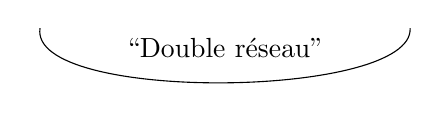
\begin{tikzpicture}[baseline=(n.base)]\node (n) {``\uline{Double réseau}''};\draw (-2.35,0.25) .. controls (-2.5,-0.7) and (2.4,-0.65) .. (2.35,0.25);\end{tikzpicture}} Supposons $S=\operatorname{Spec}k$, $k\subset\mathbb C$ extension \uline{algébrique} de $\mathbb Q$. Considérons le foncteur qui à $M$ associé
% loc: first labelled display
\begingroup\makeatletter\tagsleft@true\makeatother
\[
\bigl\{T_{\mathrm{DR}}(M),T_{\mathrm B}(M),\varphi_M\bigr\} \tag*{(4.1)}
\]
\endgroup
% loc: first comparison and question
où $\varphi:T_{\mathrm B}(M)\unsure{\otimes|\ominus}_{\mathbb Q}\mathbb C\simeq T_{\mathrm{DR}}(M)\unsure{\otimes|\ominus}_k\mathbb C$ ; ici, on ne considère pas $T_{\mathrm{DR}}(M)$ comme filtré, \deleted{et} ni $T_{\mathrm B}(M)$ muni d'une structure de Hodge. Ce foncteur est-il pl. fidèle ??

% loc: struck start and expression below it
\deleted{Il revient au $=$ de dire que}
\[
\deleted{T_{\mathrm R}(M)\cap T_{\mathrm{DR}}(M)}
\]
% loc: reduction to k with overbar
Il \deleted{est} aussitôt ramené au cas où $k=\overline{\mathbb Q}$. La question est alors équivalente à celle si le foncteur associant à $M$ le système
% loc: second labelled display
\begingroup\makeatletter\tagsleft@true\makeatother
\[
\bigl\{T_{\mathrm B}(M),\sigma\bigr\} \tag*{(4.2)}
\]
\endgroup
% loc: connexion paragraph
où $\sigma$ est la connexion canonique sur $T_{\mathrm B}(M)\otimes_{\mathbb Q}\mathbb C$, est pleinement fidèle : en effet, $\sigma$ et $T_{\mathrm{DR}}(M)$\inserted{$\subset T_{\mathrm B}(M)\unsure{\otimes|\ominus}_{\mathbb Q}\mathbb C$\unsure{,|;}} se déterminent mutuellement [$T_{\mathrm{DR}}(M)$ est l'ens. des éléments \inserted{de $T_{\mathrm B}(M)\otimes_{\mathbb Q}\mathbb C$} horizontaux pour $\sigma$ \ldots].
% loc: group description
Une autre façon de définir cette donnée, \inserted{$T_{\mathrm{DR}}\subset T_{\mathrm B}\otimes\mathbb C$,} quand on introduit le gpe de Galois $G=\underline{\operatorname{Aut}}_{\unsure{\ominus|\otimes}}(T_{\mathrm B}\deleted{\unsure{(M|M}})$ \deleted{\unsure{$\xi$} que \unsure{le}} ($M$ sous-$\otimes$-catégorie de type fini de la catégorie $\operatorname{Mot}(k)$) est la donnée de $\dot g\inG(\mathbb C)/G(\overline{\mathbb Q})$ ; si $V$ est un $G$-module (correspondant à un motif $\deleted{\unsure{V}}M$), alors
% loc: short note in left margin
\margin{\uline{NB} $G$ connexe}
% loc: lattice and inclusion
$T_{\mathrm{DR}}(M)$ n'est autre que le $\overline{\mathbb Q}$-réseau $g(V_{\overline{\mathbb Q}})\subset V\otimes_{\mathbb Q}\mathbb C$. Donc la question est simplement si pour tout $V$, l'inclusion
\[
V^G\subset V\cap g(\overline V)
\]
% loc: last lines
est une identité. [On peut supposer que $V$ est un module simple. [S'il est de dim. 1, c'est une puissance de Tate, et ça marche]] \deleted{Il revient au $=$ de}
% loc: line of dashes under the final cancellation
\par\hfill - - - - - - - - - -
% No watermark lettering securely recoverable on this image; the reading supplied by C remains an audit question.
% archive sheet number: 47



\scanpage{49}
% loc: cancelled continuation at head
\deleted{regarder $V$ seulement (où $\overline V=V\unsure{\otimes|\ominus}_{\mathbb Q}\overline{\mathbb Q}$)}
\[
\deleted{\overline V^{G}\subset\overline V\cap g(\overline V)}
\]
\deleted{et de prouver que c'est une identité [car $\overline V^G\cap V=V^G$].}

% loc: first equivalence
Or la relation $x\in\overset{\deleted{\unsure{-}}}{V}\cap g(\overline V)$ équivaut :
\begingroup\makeatletter\tagsleft@true\makeatother
\[
x\in\overset{\deleted{-}}{V},\quad g^{-1}x\in\overline V \tag*{ds}
\]
\endgroup
% loc: locus and second equivalence
et implique évidemment, si $\overline T$\inserted{$\subset\overline G$} est la \deleted{\unsure{déclinaison|clôture} de} \inserted{lieu de} $g$ sur $G_{\overline{\mathbb Q}}$
\[
x\in\overline V,\quad\deleted{\unsure{g^{-1}x}}\quad t\deleted{\unsure{^{-1}}}s^{-1}\in G_x(\mathbb C)\quad\text{pour }t,s\in\overline T(\mathbb C),
\]
et $=$ y équivaut.
% loc: stabilizer paragraph
En d'autres termes, si $G_x$ est le stabilisateur de \deleted{$G$}$x$, qui est un ss-gpe algébrique de $G$, \deleted{\unsure{on}} \inserted{la relation $x\in V\cap g(\overline W)$ équi-}vaut :
\[
\deleted{\unsure{g}}\overline R\in\overline{G_x}\deleted{\unsure{(\mathbb C)}},
\]
où $\overline R$ est l'adhérence de l'im. $\overline T\times\overline T\longrightarrow\overline G$, $(s,t)\longmapsto s^{-1}t$.

% loc: image subgroup and equality question
Or soit $\widehat R$ l'\unsure{image|im.ge} de $\overline R$ dans $G$, $H$ le sous-gr. qu'elle engendre, $H\subset G$. \deleted{Donc la propriété souhaitée équivaut à quelle \unsure{?}} La relation ds équivaut donc à $\deleted{R}H\subset G_x$ i.e. $H$ invarie $x$.
% loc: left insertion at opening of proposition
\inserted{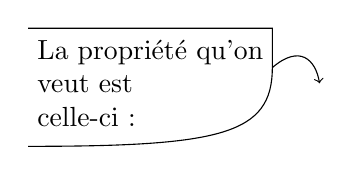
\begin{tikzpicture}[baseline=(n.base)]\node[align=left] (n) {La propriété qu'on\\veut est\\celle-ci :};\draw (-1.55,0.7) -- (1.55,0.7) -- (1.55,0.2) .. controls (1.55,-0.65) and (0.9,-0.8) .. (-1.55,-0.8);\draw[->] (1.55,0.2) .. controls (1.9,0.5) and (2.1,0.3) .. (2.15,0);\end{tikzpicture}}
% loc: heavily cancelled proposition and replacement
Pour tt $G$-module $V$, \deleted{et tt $x\in V$, tel que le stabilisateur $G_x$ contienne $R$, \inserted{i.e. tel que $R$ invarie $x$,} on a que $x\in V^G$ i.e. $G_x=G$.}
\deleted{Il suffit pour ceci que le \illegible{1} soit le ss-gpe engendré par $R$, soit égal à $G$. C'est aussi nécessaire} que les invariants de $H$ et de $G$ (pour tt repr. de $G$) soient les $=$s. Il suffit que l'on ait $H=G$, mais cette condition n'est pas nécessaire à priori, car un $k$-gpe de Borel de $G$ a cette propriété.
% loc: NB at left of cancelled lines
\margin{NB $\deleted{\unsure{\overline T}}\overline R,\overline H$ ne dépendent pas du choix de $g$ mod $G(\overline{\mathbb Q})$, \deleted{\unsure{à un près|a priori}}}
% loc: sloping note above 5
% slanted
\margin{\uline{Regarder} motifs \uline{associés} à \uline{courbes elliptiques}}
% loc: item 5, first half
5) Bien entendu, sans $=$ supposer que $k$ est alg. sur $\mathbb Q$, on peut regarder le foncteur (4.1). Mais il n'est plus en général pl. fidèle, $=$ si $k$ est de t.f. sur $\mathbb Q$, car pour $\unsure{\mathcal M|M}$ \inserted{$\otimes$-cat.} fixée de type fini $\subset\operatorname{Mot}(k)$, à condition d'agrandir $k$, on trouve que \inserted{les} $T_{\mathrm{DR}}(M)$ \uline{contiennent} $T_{\mathrm B}(M)$, donc les hom. des structures mixtes sont simplt les hom entre les $T_{\mathrm B}(M)$ : idiot !
% loc: closing lines of item 5
Pour $M$ fixé, on peut espérer tout au mieux avoir quelque résultat de disjonction de $T_{\mathrm B}$ et $T_{\mathrm{DR}}$ si $k$ est $\pm$ modérée (p.ex avoir des estimations de degré de transcendance minimum).
% No watermark lettering securely recoverable on this image; the reading supplied by C remains an audit question.
% archive sheet number: 48



\scanpage{50}
% loc: continuation of item 5
Par contre, sans hypothèse sur $k$ sauf d'être \uline{alg. clos}, il semble encore raisonnable d'espérer que (4.2) soit tjrs pleinement fidèle.
% loc: left oval
% slanted
\margin{\begin{tikzpicture}[baseline=(n.base)]\node[draw,ellipse,align=center] (n) {réseau $+$\\connexion};\end{tikzpicture}}
On est ramené pour ceci au cas $k=\mathbb C$.. C'est une conséquence de la conjecture ``du double réseau'' de 4) $+$ Tate ou Hodge, puis : 6)

% loc: item 6, main line and interlinear insertion
6) Si $S$ de type fini \inserted{sur \deleted{$\unsure{\mathbb Q}$} un corps de nbs}, on a le foncteur de 3), mais sans filtration sur $T_{\mathrm{DR}}(M)$. Il résultera\deleted{\unsure{it|t}}it de la conj. du double réseau \deleted{(qui, elle, \unsure{génér} \inserted{(de \unsure{3|?})}} que ce foncteur est pl. fidèle
% loc: closing NB
[\uline{NB} si $S$ est le spectre d'un corps de nb, cela se réduit : l'énoncé du double réseau....)
% loc: paper watermark, read sideways on this sheet
% printed form
% paper watermark, visible letters in the direction of the paper lettering
\par\noindent\textsc{\unsure{trong|rong}}\hfill\textsc{Extra}\\
\unsure{ry|y} 1808\hfill\unsure{Mauno|Maun}
% archive sheet number: 49



\scanpage{51}
% loc: heading above the rule
Remarque sur la caractérisation des classes de coh. D.R. \deleted{\unsure{qu}}\inserted{essentiellement} \uline{algébriques}. par bigraduation ou par réalité ....
\par\noindent\rule{\linewidth}{0.3pt}\par
% loc: opening and Hom insertion
$K\subset\mathbb C$ sous-corps, $M$ motif sur $K$, d'où $T_{\mathrm{DR}}(M)$. Considérons $T_{\mathrm{DR}}(M\unsure{\natural|\leftrightharpoons})$\inserted{$=\operatorname{Hom}(1,M)\otimes_{\mathbb Q}K$}, on voit que c'est un sous-module de $T_{\mathrm{DR}}(M)$, \deleted{qui est}\inserted{et que}
% loc: clauses a and b
\par a) contenu dans $T_{\mathrm{DR}}(M)_{\mathbb C}^{00}$.
\par b) \inserted{$\operatorname{Hom}(1,M)\otimes_{\mathbb Q}(K\cap\mathbb R)$ est} contenu dans $\bigl(T_{\mathrm{DR}}(M)_{\mathbb C}\bigr)_{\mathbb R}$ \deleted{[et où $\operatorname{Hom}(1,M)\otimes_{\mathbb Q}(K\cap\mathbb R)$ est contenu dans $\bigl(T_{\mathrm{DR}}(M)_{\mathbb C}\bigr)_{\mathbb R}$]}

% loc: question
A-t-on une réciproque ?

% loc: item 1, opening and group insertions
$1^\circ$) Pas pour \deleted{a) tout seul, même si}\inserted{a) et b) simultanément} $K=\mathbb Q$, si le groupe de galois motivique $G$ \inserted{pour la cat. de motifs $\unsure{\mathcal M|M}$ où on travaille} n'est pas connexe. En effet, si $G$ est \deleted{\unsure{discret}} fini [Cas des motifs effectifs de poids 0] la condition a) est vide, car $T_{\mathrm{DR}}(M)_{\mathbb C}^{00}=T_{\mathrm{DR}}(M)_{\mathbb C}$, \inserted{donc réc. de a) vraie ssi $G=(e)$.} d'autre part \deleted{b) est} la réciproque à b) est vraie ssi l'extension galoisienne $L$ de groupe $G$ de $\mathbb Q$ définie par $\mathcal M$ est \uline{tot. réelle} [on teste avec le $G$-module $M=\mathbb Q[C]$, qui donne $T_{\mathrm{DR}}(M)=L$ \ldots] ; donc dans ce cas on a une réciproque à a) et b).

% loc: connected group and embeddings
Il faut donc se borner à un $G$ connexe, ce qui suggère de regarder les réciproques pour le cas $K$ alg. clos, \inserted{p.ex. $K=\overline{\mathbb Q}$} On peut de plus renforcer la condition, en regardant \uline{toutes} les immersions $K\hookrightarrow\mathbb C$.

% loc: item 2, introductory lines
$2^\circ$) La réciproque à a) est fausse, \deleted{\unsure{même si}} ($=$ pour $\overline{\mathbb Q}$). il suffit de prendre un groupe de Galois motivique $G$ qui est un \uline{tore} de dim $\geq 3$. On voit qu'on peut trouver \inserted{sur}
% loc: pair of arrows, target, and marginal additions
$j_1,j_2:{\mathbb G_{\mathrm m\,K}}^{\unsure{p|\rho}}\rightrightarrows G'_{\deleted{\unsure{K}}\unsure{\mathbb C|K}}$\inserted{$(=\operatorname{ad}(P)$, car $G$ \unsure{comm!|commut.})} qui défnt \inserted{(pour tt $K\longrightarrow\mathbb C$)} la bigraduation de
% loc: struck margin beside the two arrows
\margin{\deleted{\uline{NB} $j_1$ et $j_2$ \unsure{proviennent} d'\unsure{un choix} de \unsure{deux} \unsure{immersions} \unsure{dans} $\mathbb C$, et \illegible{1}}}
% loc: scalar extensions and torsor
$\deleted{G}V_{\mathbb C}\simeq V'\otimes_K\mathbb C$ \quad [$V'=P\mathbin{\overset{G_K}{\deleted{\unsure{\times}}}}V$, $P\unsure{\simeq|=}\underline{\operatorname{Isom}}_{\otimes}(T_{\mathrm B}\otimes K,T_{\mathrm{DR}})$]
% loc: degree-zero representation
Donc une représentation \inserted{fidèle} de degré 0 de $G$ donne, $\deleted{V^{G'}}$ si $T$ est l'image de $(j_1,j_2):\mathbb G_{\mathrm m\,K}\times\mathbb G_{\mathrm m\,K}\mathbin{-}G'$, un $V'$ pour lequel
% loc: final equality and inequality
${V'}^{T}\inserted{(=T_{\mathrm{DR}}\cap(T_{\mathrm{DR}}\deleted{\unsure{)}}{}_{\mathbb C}^{00})}$
\inserted{\deleted{\unsure{quelque}}} est $\ne {V'}^{G'}$.
% Watermark lettering supplied by C is not recoverable on this image; retained as an audit question in the changes log.
% archive sheet number: 50



\scanpage{52}
% loc: item 3, three lines at the head
$3^\circ$) Reste la question d'une réciproque à b) si $K$ \unsure{Alg.|alg.} clos, en prenant (\inserted{\begin{tikzpicture}[baseline=(n.base)]\node[draw,ellipse,inner sep=2pt] (n) {du moins};\end{tikzpicture}} si $K\ne\overline{\mathbb Q}$) \uline{toutes} les imm. $K\longrightarrow\mathbb C$, et en conjuguant aussi au besoin avec la condition a).
% loc: paper watermark, read sideways on this sheet
% printed form
% paper watermark, visible letters in the direction of the paper lettering
\par\noindent\textsc{\unsure{ra|a} Strong}\hfill\textsc{Ex}\\
\unsure{aunoury|unoury|noury} 1808\hfill\unsure{M|A}
% archive sheet number: 51


\cotefile{15}
\scanpage{27}
\mspage{\handwritten{- 48 -}}
% archive sheet number: 26

L'élément $\handwritten{\int_\gamma}(\handwritten{\sum_k f}_k\,dx_k)$ de E ne dépend donc que de $\handwritten{a}$ et $\handwritten{z}$ et non de la route $\handwritten{\gamma}$ ; $\handwritten{a}$ restant fixe, posons $\handwritten{g}(\handwritten{z})=\handwritten{\int_\gamma}(\handwritten{\sum_k f}_k\,dx_k)$. Or, pour tout $\handwritten{z_0}\handwritten{\in}A$, il existe un polycylindre P de centre $\handwritten{z_0}$, contenu dans A, et une fonction holomorphe $\handwritten{u}$ dans P telle que $\handwritten{u}(\handwritten{z_0})=\handwritten{g}(\handwritten{z_0})$ et $d\handwritten{u}=\handwritten{\sum_k f}_k\,dx_k$ dans P ; si pour $\handwritten{z}\handwritten{\in}P$, $\handwritten{\sigma}$ est la route linéaire $t\handwritten{\to z_0}+t(\handwritten{z}-\handwritten{z_0})$ $(t\handwritten{\in[}0,1\handwritten{]})$, on a donc $\handwritten{u}(\handwritten{z})-\handwritten{u}(\handwritten{z_0})=\handwritten{\int_\sigma}(\handwritten{\sum_k f}_k\,dx_k)=\handwritten{g}(\handwritten{z})-\handwritten{g}(\handwritten{z_0})$, d'où $\handwritten{g}(\handwritten{z})=\handwritten{u}(\handwritten{z})$ dans P, ce qui démontre la proposition.

En particulier, si $n=1$, on voit que toute fonction holomorphe $\handwritten{f}$ dans un domaine \uline{contractile} $A\handwritten{\subset}K$ admet une primitive $\handwritten{g}$ holomorphe dans A, c'est-à-dire une fonction dont la dérivée $\handwritten{g}'=\handwritten{f}$ dans A ; en outre, si $\handwritten{g}_1$ et $\handwritten{g}_2$ sont deux primitives de $\handwritten{f}$ dans A, leur différence est \deleted{\unsure{nulle|même}} constante dans un voisinage d'un point quelconque de A, donc constante dans A puisque A est connexe.

Une variante de la démonstration du th.1 et de la prop.2 consiste à établir d'abord un principe général de prolongement analytique, de la façon suivante :

\uline{Etant donné un domaine} $A\handwritten{\subset}K^n$, \uline{on suppose donnée en chaque point} $\handwritten{z}\handwritten{\in}A$, \uline{une famille} $\handwritten{\Phi}(\handwritten{z})$ \uline{de polycylindres ouverts contenus dans A et de centre} $\handwritten{z}$, \uline{et pour tout} $P\handwritten{\in\Phi}(\handwritten{z})$, \uline{une fonction holomorphe} $\handwritten{u}_{p}$ \uline{définie dans} P ; \uline{on suppose que pour tout} $\handwritten{x\in}P\handwritten{\in\Phi}(\handwritten{z})$ \uline{il existe} $Q\handwritten{\in\Phi}(\handwritten{x})$ \uline{tel que} $\handwritten{u}_Q(\handwritten{x})=\handwritten{u}_P(\handwritten{x})$ ; \uline{on suppose en outre que si} $P\handwritten{\in\Phi}(\handwritten{z})$, $Q\handwritten{\in\Phi}(\handwritten{z}')$ \uline{ont une intersection non vide et si} $\handwritten{u}_P(\handwritten{x})=\handwritten{u}_Q(\handwritten{x})$ \uline{en un point de} $P\handwritten{\cap}Q$, \uline{alors} $\handwritten{u}_P$ \uline{et} $\handwritten{u}_Q$ \uline{sont identiques dans} $P\handwritten{\cap}Q$ ; \uline{enfin}, \uline{si}


\scanpage{29}
\mspage{\handwritten{- 47 -}}
% archive sheet number: 28

en particulier $\handwritten{\int_\gamma}d\handwritten{g}=0$ le long de tout \uline{circuit} dans A.

PROPOSITION 2.- \uline{Soit} $A\handwritten{\subset}K^n$ \uline{un domaine} contractile, \uline{et soit} $\handwritten{\sum_{k=1}^n f}_k\,dx_k$ \uline{une expression différentielle fermée à coefficients holomorphes dans} A. \uline{Il existe alors une fonction} $\handwritten{g}$ \uline{holomorphe dans} A \uline{et telle que} $d\handwritten{g}=\handwritten{\sum_{k=1}^n f}_k\,dx_k$.

Nous utiliserons le lemme suivant :

\uline{Lemme 1}.- \uline{Quels que soient les points} $\handwritten{a}$, $\handwritten{b}$ \uline{d'un domaine} $A\handwritten{\subset}K^n$, \uline{il existe une route a-chevée linéaire par morceaux}, \uline{contenue dans} A \uline{et ayant pour extrémités} $\handwritten{a}$ \uline{et} $\handwritten{b}$.

Il suffit de prouver que l'ensemble B des extrémités des routes linéaires par morceaux contenues dans A et d'origine A, est à la fois ouvert et fermé. \handwritten{O}r, si $\handwritten{c\in}\overline{B}$, il existe une boule S de centre $\handwritten{c}$ contenue dans A et contenant une extrémité $\handwritten{b}$ d'une route $\handwritten{\gamma}$ d'origine $\handwritten{a}$ contenue dans A. Comme le segment d'extrémités $\handwritten{b}$ et $\handwritten{c}$ est contenu dans S, donc dans A, $\handwritten{c}$ est l'extrémité d'une route linéaire par morceaux, juxta-position de $\handwritten{\gamma}$ et d'une route linéaire. De même, tout point $\handwritten{x\in}S$ est extrémité d'une route linéaire par morceaux, juxtaposition de $\handwritten{\gamma}$ et d'une route linéaire, donc $S\handwritten{\subset}C$, ce qui prouve que C est ouvert et fermé. Ce lemme étant démontré, soit $\handwritten{a}$ un point quelconque de A, $\handwritten{z}$ un point quelconque de A, $\handwritten{\gamma}$ et $\handwritten{\gamma}'$ deux routes contenues dans A d'origine $\handwritten{a}$ et d'extrémité $\handwritten{z}$ (il en existe en vertu du lemme). On a $\handwritten{\int_\gamma}(\handwritten{\sum_k f}_k\,dx_k)=\handwritten{\int_{\gamma'}}(\handwritten{\sum_k f}_k\,dx_k)$. En effet, si $\handwritten{\gamma}$ est définie dans un intervalle $\handwritten{[}b,c\handwritten{]}$, on peut, en remplaçant $\handwritten{\gamma}'$ par une route équivalente, supposer que $\handwritten{\gamma}'$ est définie dans un intervalle de la forme $\handwritten{[}c,d\handwritten{]}$ ; on a $\handwritten{\gamma}(c)=\handwritten{\gamma}'(d)=\handwritten{z}$ ; on peut donc définir $\handwritten{\gamma}''$ dans $\handwritten{[}b,d\handwritten{]}$, en posant $\handwritten{\gamma}''(t)=\handwritten{\gamma}(t)$ dans $\handwritten{[}b,c\handwritten{]}$ et $\handwritten{\gamma}''(t)=\handwritten{\gamma}'(c+d-t)$ dans $\handwritten{[}c,d\handwritten{]}$ ; comme $\handwritten{\gamma}''(d)=\handwritten{\gamma}'(c)=\inserted{\handwritten{a=}}\handwritten{\gamma}''(b)$, $\handwritten{\gamma}''$ est un \uline{circuit}, et notre assertion résulte du th.\unsure{1|2}.


\scanpage{31}
\mspage{\handwritten{- 46 -}}
% archive sheet number: 30

COROLLAIRE.- \uline{Soient} $\handwritten{\gamma}$ \uline{et} $\handwritten{\gamma}'$ \uline{deux routes achevées à valeurs dans} A, \uline{ayant même origine} $\handwritten{a}$ \uline{et même extrémité} $\handwritten{b}$, \uline{et telles qu'il existe une déformation de} $\handwritten{\gamma}$ \uline{en} $\handwritten{\gamma}'$ \uline{dans} A \uline{qui laisse fixes} $\handwritten{a}$ \uline{et} $\handwritten{b}$. \uline{Alors}, \uline{si l'expression différentielle} $\handwritten{\sum_k f}_k\,dx_k$ \uline{satisfait aux conditions} (1), \uline{on a} $\handwritten{\int_\gamma}(\handwritten{\sum_k f}_k\,dx_k)=\handwritten{\int_{\gamma'}}(\handwritten{\sum_k f}_k\,dx_k)$.

On peut supposer que $\handwritten{\gamma}$ et $\handwritten{\gamma}'$ sont définies dans le même intervalle $I=\handwritten{[\alpha,\beta]}$ ; soit $\handwritten{\gamma}^{\unsure{o|0|\circ}}$ l'opposé de $\handwritten{\gamma}$, et $\handwritten{\gamma}_1(t)=\handwritten{\gamma}_{\handwritten{\unsure{o|0|\circ}}}(t-\handwritten{\beta}+\handwritten{\alpha})$ un chemin équivalent à $\handwritten{\gamma}^{\handwritten{\unsure{o|0|\circ}}}$ défini dans $I+(\handwritten{\beta}-\handwritten{\alpha})$. Les routes $\handwritten{\gamma\vee\gamma}_1$ et $\handwritten{\gamma}'\handwritten{\vee\gamma}_1$ sont des circuits dans A et peuvent évidemment être déformés l'un en l'autre dans A en vertu des hypothèses ; en leur appliquant le th.1, on a aussitôt le corollaire.

\unsure{DÉFINITION|DÈFINITION} 5.- \uline{On dit qu'un domaine} $A\handwritten{\subset}K^n$ \uline{est contractile si tout lacet dans} A \uline{peut être déformé dans} A \uline{en un point de} A.

Par exemple, tout domaine \uline{étoilé} par rapport à un point est contractile.

Une expression différentielle $\handwritten{\sum_{k=1}^n f}_k\,dx_k$ à coefficients holomorphes dans un domaine A est dite \uline{fermée} si elle satisfait aux conditions (1). On voit donc que :

\unsure{THÈORÈME|THÉORÈME|THÈORÉME|THÉORÉME} 2 (Cauchy).- \uline{Dans un domaine contractile l'intégrale d'une expression différentielle fermée} (à coefficients holomorphes) \uline{le long d'un circuit quelconque est nulle}.

On peut évidemment, pour le cas des variables \uline{réelles}, généraliser le th.1 au cas où les $\handwritten{f}_k$ sont seulement supposées continument différentiables ; est-ce que cela en vaut la peine ?

\handwritten{\unsure{3|2}}. \uline{Primitives d'une fonction holomorphe}.

Soit $A\handwritten{\subset}K^n$ un domaine \uline{quelconque}, $\handwritten{g}$ une fonction holomorphe dans A ; si on pose $d\handwritten{g}=\handwritten{\sum_{k=1}^n f}_k\,dx_k$, il est immédiat que cette expression différentielle est \uline{fermée} ; en outre, en vertu des définitions, le long d'une route $\handwritten{\gamma}$ définie dans $I=\qquad$, on a $\handwritten{\int_\gamma}d\handwritten{g}=\handwritten{\int_\gamma}(\handwritten{\sum_k f}_k\,dx_k)=\handwritten{g}(\handwritten{\gamma}(\handwritten{\beta}))-\handwritten{g}(\handwritten{\gamma}(\handwritten{\alpha}\unsure{)|))|}$
% The source leaves the space after I= blank. At the right edge a faint arc may be one closing parenthesis; a second, or no intentional closing stroke, remains possible. Accents on DEFINITION and THEOREME are handwritten over the typed E letters.


\scanpage{33}
\mspage{\handwritten{- 44 -}}
% archive sheet number: 32

chacune des fonctions $\handwritten{f}_k$ soit égale à une série entière sommable par rapport aux $x_j-a_{ij}$. Il existe un nombre $\handwritten{\rho>}0$ tel que, pour tout $\handwritten{x\in\varphi}(I\handwritten{\times}J)$, le polycylindre ouvert de centre $\handwritten{x}$ et de rayons $\handwritten{\rho}$ soit contenu dans un $P_i$ au moins ; car si $\handwritten{\delta}(\handwritten{x})$ désigne la plus grande distance de $\handwritten{x}$ aux frontières de ceux des $P_i$ qui contiennent $\handwritten{x}$, on vérifie aussitôt que $\handwritten{\delta}(\handwritten{x})$ est continue dans $\handwritten{\varphi}(I\handwritten{\times}J)$ et est $\handwritten{>}0$ en tout point, donc atteint son minimum $\handwritten{\rho}$ en un point de $\handwritten{\varphi}(I\handwritten{\times}J)$, ce qui implique $\handwritten{\delta}(\handwritten{x})\handwritten{\geq\rho>}0$ pour tout $\handwritten{x\in\varphi}(I\handwritten{\times}J)$. Par suite, pour tout $\handwritten{x\in\varphi}(I\handwritten{\times}J)$, chacune des fonctions $\handwritten{f}_k$ est égale à une série entière sommable (par rapport aux $z_j-\handwritten{x}_j$) dans le polycylindre ouvert de centre $\handwritten{x}$ et de rayon $\handwritten{\rho}$ (chap.I, \handwritten{\S}1, prop.\handwritten{\unsure{4|14}}). En vertu de la continuité uniforme de $\handwritten{\varphi}$, il existe $\handwritten{\varepsilon>}0$ tel que les relations $\handwritten{|}t-t'\handwritten{|}\handwritten{\leq\varepsilon}$, $\handwritten{|}s-s'\handwritten{|}\handwritten{\leq\varepsilon}$ entraînent $\handwritten{\|\varphi}(t,s)-\handwritten{\varphi}(t',s')\handwritten{\|\leq\frac{\rho}{4}}$. Soit $(t_{\handwritten{\alpha}})$ $(0\handwritten{\leq\alpha\leq}p)$ une suite croissante de points de I tels que $t_0=a$, $t_p=b$ et $t_{\handwritten{\alpha}+1}-t_{\handwritten{\alpha}}\handwritten{\leq\varepsilon}$ pour $0\handwritten{\leq\alpha\leq}p-1$ ; soit de même $(s_{\handwritten{\beta}})$ $(0\handwritten{\leq\beta\leq}q)$ une suite croissante de points de J tels que $s_0=c$, $s_q=d$ et $s_{\handwritten{\beta}+1}-s_{\handwritten{\beta}}\handwritten{\leq\varepsilon}$ pour $0\handwritten{\leq\beta\leq}q-1$. Désignons par $\handwritten{\gamma_\beta}$ le circuit défini par
\[
\begin{aligned}
\handwritten{\gamma_\beta}(t)&=\handwritten{\varphi}(t_{\handwritten{\alpha}},s_{\handwritten{\beta}})+\frac{t-t_{\handwritten{\alpha}}}{t_{\handwritten{\alpha}+1}-t}\bigl(\handwritten{\varphi}(t_{\handwritten{\alpha}+1},s_{\handwritten{\beta}})-\handwritten{\varphi}(t_{\handwritten{\alpha}},s_{\handwritten{\beta}})\bigr)\quad\text{pour }t_{\handwritten{\alpha}}\handwritten{\leq}t\handwritten{\leq}t_{\handwritten{\alpha}+1}\\
&0\handwritten{\leq\alpha\leq}p-1,\quad1\handwritten{\leq\beta\leq}q-1
\end{aligned}
\]
; on posera en outre $\handwritten{\gamma}_0=\handwritten{\gamma}$, $\handwritten{\gamma}_q=\handwritten{\gamma}'$. Tout revient à prouver que l'on a, pour $0\handwritten{\leq\beta\leq}q-1$, $\handwritten{\int_{\gamma_\beta}}(\handwritten{\sum_k f}_k\,dx_k)=$ $=\handwritten{\int_{\gamma_{\beta+1}}}(\handwritten{\sum_k f}_k\,dx_k)$. Or, pour chaque indice $\handwritten{\alpha}$ tel que $0\handwritten{\leq\alpha\leq}p-1$, les points $\handwritten{\gamma_\beta}(t)$ et $\handwritten{\gamma_{\beta+1}}(t)$ pour $t_{\handwritten{\alpha}}\handwritten{\leq}t\handwritten{\leq}t_{\handwritten{\alpha}+1}$ appartiennent tous à un même polycylindre ouvert $Q_{\handwritten{\alpha},\handwritten{\beta}}$ de centre un point de $\handwritten{\varphi}(I\handwritten{\times}J)$ et de rayons $\handwritten{\rho}$ (fig.1) ; on sait d'autre part qu'il existe dans $Q_{\handwritten{\alpha\beta}}$


\scanpage{35}
\mspage{\handwritten{- 42 -}}
% archive sheet number: 34

convenable $s\handwritten{\to}s+a$ et la déformation $(t,s)\handwritten{\to\varphi}_2(t,s+a)$ de $\handwritten{\gamma}_1$ en $\handwritten{\gamma}_2$ ; alors si $\handwritten{\varphi}$ est la fonction égale à $\handwritten{\varphi}_1$ dans $I\handwritten{\times}J_1$ et à $\handwritten{\varphi}_2$ dans $I\handwritten{\times}J_2$ (ce qui a un sens; puisque les deux fonctions coïncident sur $I\handwritten{\times}(J_1\handwritten{\cap}J_2)$), il est clair que $\handwritten{\varphi}$ est continue dans $I\handwritten{\times}(J_1\handwritten{\cup}J_2)$ et est une déformation de $\handwritten{\gamma}_0$ en $\handwritten{\gamma}_2$ dans A. Comme en outre tout chemin est déformable en lui-même (en prenant $\handwritten{\varphi}(t,s)=\handwritten{\gamma}(t)$ pour tout $s\handwritten{\in}J$), la relation ``$\handwritten{\gamma}$ est déformable en $\handwritten{\gamma}'$ dans A'' est une \uline{relation d'équivalence} entre les chemins définis dans I et à valeurs dans A.

\uline{Exemple}.- On dit qu'un domaine $A\handwritten{\subset\mathbb{R}}^n$ est \uline{étoilé} par rapport à un point $\handwritten{a\in}A$ si pour tout $\handwritten{x\in}A$, le segment fermé d'extrémités $\handwritten{a}$ et $\handwritten{x}$ est contenu dans A. Dans un domaine étoilé par rapport à A, \uline{tout chemin} (resp. \uline{tout lacet}) $\handwritten{\gamma}$ \uline{est déformable en le point} $\handwritten{a}$ par la déformation $\handwritten{\varphi}(t,s)=\handwritten{a}+(1-s)(\handwritten{\gamma}(t)-\handwritten{a})$ (pour $0\handwritten{\leq}s\handwritten{\leq}1$). Deux chemins (resp. lacets) quelconques sont donc déformables l'un en l'autre dans A.

\uline{Remarque}.- Si $\handwritten{\gamma}$ est une juxta-position de deux chemins $\handwritten{\gamma}_1$, $\handwritten{\gamma}_2$, et $\handwritten{\varphi}$ une déformation de $\handwritten{\gamma}$ en $\handwritten{\gamma}'$ dans A, $\handwritten{\gamma}'$ est juxtaposition des deux chemins $\handwritten{\gamma}'_1$, $\handwritten{\gamma}'_2$ déformés de $\handwritten{\gamma}_1$, $\handwritten{\gamma}_2$ par $\handwritten{\varphi}$. Mais on aura soin d'observer que si $\handwritten{\gamma}_1$ et $\handwritten{\gamma}_2$ peuvent être \uline{chacun} déformés \margin{\handwritten{2}}dans A en deux nouveaux chemins $\handwritten{\gamma}'_1$\unsure{,|} $\handwritten{\gamma}'_2$, tels que l'extrémité de $\handwritten{\gamma}'_1$ soit l'origine de $\handwritten{\gamma}'_2$, il ne s'ensuit nullement que $\handwritten{\gamma}$ puisse être déformé dans A en la juxtaposition de $\handwritten{\gamma}'_1$ et de $\handwritten{\gamma}'_2$.

PROPOSITION 1.- \uline{Tout chemin achevé dans} A \uline{peut être déformé dans} A \uline{en une route linéaire par morceaux ayant mêmes extrémités}.

En effet, soit $\handwritten{\gamma}$ un chemin a chevé à valeurs dans A, défini dans l'intervalle compact $I=\handwritten{[}a,b\handwritten{]}$. L'ensemble $\handwritten{\gamma}(I)$ est compact et contenu dans A ; la distance $\handwritten{\rho}$ de cet ensemble à $\handwritten{\complement}A$ est donc $\handwritten{>}0$.


\scanpage{37}
\mspage{- \handwritten{31} -}
% archive sheet number: 36

\begin{center}
CHAPITRE II (Etat 1)

FONCTIONS HOLOMORPHES D'UNE VARIABLE COMPLEXE.

\handwritten{\S}1. Le principe du prolongement analytique.
\end{center}

\uline{\handwritten{1}}. \uline{Prolongement analytique \unsure{.|}d'une fonction holomorphe}.

Dans ce \handwritten{\S}\unsure{,|;} K désignera \uline{le corps des nombres réels ou le corps des nombres complexes}, E un espace normé complet sur K.

PROPOSITION 1.- \uline{Dans l'espace} $K^p$, \uline{soient} P \uline{et} Q \uline{deux polycylindres ouverts}, \uline{de centres} $\handwritten{a}$ \uline{et} $\handwritten{b}$, \uline{tels que} $P\handwritten{\cap}Q$ \uline{ne soit pas vide}. \uline{Soient} $\handwritten{f}(\handwritten{x})=\handwritten{\sum c}_{n_1n_2..n_p}(x_1-a_1)^{n_1}\ldots(x_p-a_p)^{n_p}$ \uline{la somme d'une série entière par rapport aux} $x_i-a_i$, \uline{sommable dans} P, \uline{et} $\handwritten{g(}\deleted{\handwritten{g}}\inserted{\handwritten{x}}\handwritten{)}\handwritten{=}$ $=\handwritten{\sum d}_{n_1n_2..n_p}(x_1-b_1)^{n_1}\ldots(x_p-b_p)^{n_p}$ \uline{la somme d'une série entière par rapport aux} $x_i-b_i$, \uline{sommable dans} Q. \uline{S'il existe un ensemble ouvert non vide} $U\handwritten{\subset}P\handwritten{\cap}Q$ \uline{tel que} $\handwritten{f}(\handwritten{x})=\handwritten{g}(\handwritten{x})$ \uline{pour tout} $\handwritten{x\in}U$, \uline{on a} $\handwritten{f}(\handwritten{x})=\handwritten{g}(\handwritten{x})$ \uline{pour} tout $\handwritten{x\in}P\handwritten{\cap}Q$.

Soit en effet $\handwritten{x}$ un point de U et $\handwritten{y}$ un point quelconque de $P\handwritten{\cap}Q$ ; le segment fermé d'extrémités $\handwritten{x}$ et $\handwritten{y}$ appartient tout entier à $P\handwritten{\cap}Q$, qui est convexe ; la fonction $\handwritten{h}(t)=\handwritten{f}(\handwritten{x}+t(\handwritten{y}-\handwritten{x}))-\handwritten{g}(\handwritten{x}+t(\handwritten{y}-\handwritten{x}))$ est donc une fonction holomorphe de la variable réelle t dans un intervalle ouvert I contenant $\handwritten{[}0,1\handwritten{]}$. Désignons par $\handwritten{\rho}$ la borne supérieure de l'ensemble A des t tels que $0\handwritten{\leq}t\handwritten{\leq}1$ et que $\handwritten{h}(s)=0$ pour $0\handwritten{\leq}s\handwritten{\leq}t$ ; on a par hypothèse $\handwritten{\rho>}0$, et il est clair par continuité que $\handwritten{\rho\in}A$ ; nous allons montrer que $\handwritten{\rho}=1$ ce qui démontrera la proposition. Dans le cas contraire, la fonction $\handwritten{h}(t)$ serait égale à la somme d'une série entière en $t-\handwritten{\rho}$, convergente dans un intervalle ouvert de centre $\handwritten{\rho}$ ; mais on a $\handwritten{h}(t)=0$ pour tout t tel que $0\handwritten{\leq}t\handwritten{\leq\rho}$, donc d'après le principe des zéros isolés, les coefficients de cette série en $t-\handwritten{\rho}$ sont tous nuls on a donc aussi $\handwritten{h}(t)=0$ pour $\handwritten{\rho<}t\handwritten{<\rho}+\handwritten{\alpha}$, où $\handwritten{\alpha>}0$ ; mais cela est


\scanpage{39}
\mspage{- 29 -}
% archive sheet number: 38

\[
\begin{aligned}
\frac{\handwritten{\partial}}{\handwritten{\partial}x_k}\left(\frac{\handwritten{\partial u}_j}{\handwritten{\partial}x_i}\right)&=\frac{\handwritten{\partial}U_{ij}}{\handwritten{\partial}x_k}(\handwritten{x};\handwritten{u}(\handwritten{x}))+\handwritten{\sum_{\unsure{k|h}=1}^q}\frac{\handwritten{\partial}U_{ij}}{\handwritten{\partial}y_h}(\handwritten{x};\handwritten{u}(\handwritten{x}))\mathbin{.}\frac{\handwritten{\partial u}_h}{\handwritten{\partial}x_k}
&& (1\handwritten{\leq}i\handwritten{\leq}p,\\
&=\frac{\handwritten{\partial}U_{ij}}{\handwritten{\partial}x_k}(\handwritten{x};\handwritten{u}(\handwritten{x}))+\handwritten{\sum_{\unsure{k|h}=1}^q}\frac{\handwritten{\partial}U_{ij}}{\handwritten{\partial}y_h}(\handwritten{x};\handwritten{u}(\handwritten{x}))U_{kh}(\handwritten{x};\handwritten{u}(\handwritten{x})).
&&1\handwritten{\leq}k\handwritten{\leq}p,\\
&&&1\handwritten{\leq}j\handwritten{\leq}q
\end{aligned}
\]

Ecriva\handwritten{-}nt que les expressions ainsi obtenues pour $\frac{\handwritten{\partial}}{\handwritten{\partial}x_k}(\frac{\handwritten{\partial u}_j}{\handwritten{\partial}x_i})$ et $\frac{\handwritten{\partial}}{\handwritten{\partial}x_i}(\frac{\handwritten{\partial u}_j}{\handwritten{\partial}x_k})$ sont égales au point $\handwritten{x}$, puis faisant $\handwritten{x}=\handwritten{x}_0$ et tenant compte de (23) il vient
\[
\begin{aligned}
&\frac{\handwritten{\partial}U_{ij}}{\handwritten{\partial}x_k}(\handwritten{x}_0;\handwritten{y}_0)+\handwritten{\sum_{h=1}^q}\frac{\handwritten{\partial}U_{ij}}{\handwritten{\partial}y_h}(\handwritten{x}_0;\handwritten{y}_0)U_{kh}(\handwritten{x}_0;\handwritten{y}_0)=\\
&=\frac{\handwritten{\partial}U_{kj}}{\handwritten{\partial}x_i}(\handwritten{x}_0;\handwritten{y}_0)+\handwritten{\sum_{\unsure{k|h}=1}^q}\frac{\handwritten{\partial}U_{kj}}{\handwritten{\partial}y_h}(\handwritten{x}_0;\handwritten{y}_0)U_{jh}(\handwritten{x}_0;\handwritten{y}_0)
\end{aligned}
\]
Mais comme par hypothèse, $(\handwritten{x}_0,\handwritten{y}_0)$ est un point arbitraire de A, on obtient bien (24).

$2^{\handwritten{\circ}}$ Les conditions sont \uline{suffisantes}. Considérons l'équation différentielle
\[
\handwritten{y}'=\underline{U}(\handwritten{x}_0+t(\handwritten{x}-\handwritten{x}_0);\handwritten{y})\mathbin{.}(\handwritten{x}-\handwritten{x}_0)\tag*{(25)}
\]

où $\underline{U}$ est la matrice $(U_{ij})$, $\handwritten{x}_0$ et $\handwritten{x}$ sont fixés dans B, et $\handwritten{y}'=d\handwritten{y}/dt$, t variant dans un voisina ge de 0 dans K. Il résulte de la formation de la série majorante dans la démonstration du th.2 que, dès que $\handwritten{x}-\handwritten{x}_0$ est assez petit, l'équation (25) admet une solution t une seule $\handwritten{v}(t;\handwritten{x}_0,\handwritten{x},\handwritten{y}_0)$ holomorphe pour $\handwritten{|}t\handwritten{|<}2$ et pour $\handwritten{x}$ et $\handwritten{x}_0$ dans un voisinage assez petit U de $\handwritten{a}$, $\handwritten{y}_0$ dans un voisinage assez petit V de $\handwritten{b}$ et telle que $\handwritten{v}(0;\handwritten{x}_0,\handwritten{x},\handwritten{y}_0)=\handwritten{y}_0$. Si $\handwritten{v}=(v_j)$, on a donc
\[
\frac{dv_j}{dt}=\handwritten{\sum_{i=1}^p}U_{ij}(\handwritten{x}_0+t(\handwritten{x}-\handwritten{x}_0);\handwritten{v}(t))(x_i-x_{i0})\qquad(1\handwritten{\leq}j\handwritten{\leq}q)\tag*{(26)}
\]
On déduit de là que
\[
\begin{aligned}
\frac{d}{dt}\left(\frac{\handwritten{\partial}v_j}{\handwritten{\partial}x_k}\right)&=\frac{\handwritten{\partial}}{\handwritten{\partial}x_k}\left(\frac{dv_j}{dt}\right)=U_{kj}(\handwritten{x}_0+t(\handwritten{x}-\handwritten{x}_0);\handwritten{v}(t))+\\
&\quad+t\handwritten{\sum_i}(x_i-x_{i0})\frac{\handwritten{\partial}U_{ij}}{\handwritten{\partial}x_k}(\handwritten{x}_0+t(\handwritten{x}-\handwritten{x}_0);\handwritten{v}(t))\\
&\quad+\handwritten{\sum_{i,h}}(x_i-x_{i0})\frac{\handwritten{\partial}U_{ij}}{\handwritten{\partial}y_h}(\handwritten{x}_0+t(\handwritten{x}-\handwritten{x}_0);\handwritten{v}(t))\frac{\handwritten{\partial}v_{\unsure{n|h}}}{\handwritten{\partial}x_k}
\qquad(1\handwritten{\leq}j\handwritten{\leq}q,\ 1\handwritten{\leq}k\handwritten{\leq}p)
\end{aligned}
\]


\scanpage{41}
\mspage{- 27 -}
% archive sheet number: 40

\[
D\handwritten{u}(x,x_0,\handwritten{y}_0)=\handwritten{f}(x,\handwritten{u}(x,x_0,\handwritten{y}_0))\tag*{(20)}
\]
(D \uline{dériva tion par rapport à} x, $\handwritten{f}=(f_i)$), \uline{et la condition}
\[
\handwritten{u}(x_0,x_0,\handwritten{y}_0)=\handwritten{y}_0.\tag*{(21)}
\]

\uline{En outre}, \uline{il existe un voisinage} $V_1\handwritten{\subset}V$ \uline{de} $\handwritten{b}$ \uline{tel que}, \uline{pour tout} $\handwritten{y}_0\handwritten{\in}V_1$ \uline{et tout couple de points} $x,x_0$ \uline{de} U, \uline{l'équation} $\handwritten{y}_0=\handwritten{u}(x_0,x,\handwritten{y})$ \uline{ait dans} V \uline{une seule ra-cine} $\handwritten{y}=\handwritten{u}(x,x_0,\handwritten{y}_0)$.

Posons en effet $x-x_0=t$, $\handwritten{y}-\handwritten{y}_0=\handwritten{z}$ ; l'équation différentielle $\handwritten{y}'=\handwritten{f}(x,\handwritten{y})$ devient $\handwritten{z}'=\handwritten{f}(x_0+t,\handwritten{y}_0+\handwritten{z})$, et le second membre est holomorphe pour $(t,\handwritten{z})$ dans un voisinage de 0 dans $K^{p+1}$ et $(x_0,\handwritten{y}_0)$ dans un voisinage de $(a,\handwritten{b})$ ; la condition (21), pour une intégrale $\handwritten{v}$ de cette équation, s'écrit $\handwritten{v}(0;x_0,\handwritten{y}_0)=0$. On est donc dans les conditions d'application du th.2, d'où la première partie de la proposition. D'autre pa\handwritten{-}rt, si U a été pris assez petit, il existe un voisinage $V_1\handwritten{\subset}V$ de $\handwritten{b}$ tel que, pour tout $x_0\handwritten{\in}U$ et tout $\handwritten{y}_0\handwritten{\in}V_1$, l'image de U par l'application $x\handwritten{\to u}(x,x_0,\handwritten{y}_0)$ est contenue dans V car si M est le maximum de $\handwritten{\|f}(x,\handwritten{y})\handwritten{\|}$ dans $U\handwritten{\times}C$, on a en vertu du th. des accroissements finis, $\handwritten{\|u}(x,x_0,\handwritten{y}_0)-\handwritten{y}_0\handwritten{\|}=\handwritten{\|u}(x,x_0,\handwritten{y}_0)-\handwritten{u}(x_0,x_0,\handwritten{y}_0)\handwritten{\|\leq}M\handwritten{|}x-x_0\handwritten{|}$ quels que soient x et $x_0$ dans U. Si $\handwritten{y}=\handwritten{u}(x,x_0,\handwritten{y}_0)\handwritten{\in}V$, la fonction $s\handwritten{\to u}(s,x,\handwritten{y})$ est donc définie dans U et prend la valeur $\handwritten{y}$ au point x ; elle est donc égale à $\handwritten{u}(s,x_0,\handwritten{y}_0)$ en raison du th.2, et on a donc $\handwritten{u}(x_0,x,\handwritten{y})=\handwritten{u}(x_0,x_0,\handwritten{y}_0)=\handwritten{y}_0$. D'ailleurs, si $\handwritten{\unsure{w|W}\in}V$ est tel que $\handwritten{y}_0=\handwritten{u}(x_0,x,\handwritten{\unsure{w|W}})$, l'intégrale $s\handwritten{\to u}(s,x,\handwritten{\unsure{w|W}})$ qui est définie dans U, prend la valeur $\handwritten{y}_0$ au point $x_0$,donc est égale à $\handwritten{u}(s,x_0,\handwritten{y}_0)$ ; en particulier, elle prend la valeur $\handwritten{y}$ au point x, ce qui montre que $\handwritten{y}=\handwritten{\unsure{w|W}}$ et achève la démonstration.


\scanpage{43}
\mspage{- 24 -}
% archive sheet number: 42

\[
\left\{\begin{aligned}
m-1&=n+\handwritten{\sum_{j=1}^p\sum_{k=1}^{r_j}}s_{kj}\\
\handwritten{\mu_\ell}&=\handwritten{\unsure{\lambda|\Lambda}_\ell}+\handwritten{\sum_{j=1}^p\sum_{k=1}^{r_j}\nu}_{kj}\qquad(1\handwritten{\leq\ell\leq}q)
\end{aligned}\right.\tag*{(16)}
\]
On tire de ces conditions que
\[
m+\handwritten{\sum_{\ell=1}^q\mu_\ell}=1+n+\handwritten{\sum_{\ell=1}^q\lambda_\ell}+\handwritten{\sum_{j=1}^p\sum_{k=1}^{r_j}}(s_{kj}+\handwritten{\sum_{\ell=1}^q\nu}_{kj\handwritten{\ell}})
\]
et par suite, pour tout système d'exposants $(s_{kj},\handwritten{\nu}_{kj1},..,\handwritten{\nu}_{kjq})$ qui figure aux seconds membres de (16), on a $s_{kj}+\handwritten{\sum_{\ell=1}^q\nu}_{kj\handwritten{\ell}}\handwritten{<}m+\handwritten{\sum_{\ell=1}^q\mu_\ell}$ ; en d'autres termes, et comme K est de caractéristique 0, les relations (15) déterminent les coefficients des termes de degré \uline{total} t dans $u_i$ en fonction de ceux des termes de degré total $\handwritten{<}t$ dans les $u_j$ $(1\handwritten{\leq}j\handwritten{\leq}p)$ ; par récurrence sur t, on voit donc que les équations (15) déterminent les coefficients $h_i(m;\handwritten{\mu}_1,..,\handwritten{\mu}_q)$ de fa\handwritten{-}çon \uline{unique}, ce qui montre déjà que si le problème est possible, il n'a qu'une seule solution. En outre, si les $h_i(m;\handwritten{\mu}_1,..,\handwritten{\mu}_q)$ sont déterminés par récurrence à partir des relations (15), les séries entières ayant ces coefficients seront solutions du problème \uline{pourvu qu'elles soient sommables dans un\unsure{voisina}\handwritten{-}ge de l'origine} dans $K^{q+1}$ ; . En effet, s'il en est ainsi, ces séries sont fonctions continues dans un voisina ge de l'origine, donc on peut trouver un tel voisinage $U\handwritten{\times}W$ dont l'image par $(x;z_1,..,z_q)\handwritten{\to}(u_i(x;z_1,\ldots,z_q))$ soit contenue dans P, et tel que les séries $u_i$ soient substituables dans (14) pour $x\handwritten{\in}U$, $(z_1,\ldots,z_q)\handwritten{\in}W$ (\handwritten{\S}1,th.2) ; l'expression de la dérivée d'une série entière et les relations (15) montreront alors que les $u_i$ sont bien solutions du système (12) dans $U\handwritten{\in}W$.

Pour prouver la somm bilité des séries $u_i$, considérons pour chacune des séries (14), une série majorante, dont nous désignerons les coefficients par $G_i(n;r_1,..,r_p;\handwritten{\lambda}_1,\ldots,\handwritten{\lambda}_q)$ ; déterminons alors les coefficients $H_i(m;\handwritten{\mu}_1,\ldots,\handwritten{\mu}_q)$ par les conditions


\scanpage{45}
\mspage{- 23 -}
% archive sheet number: 44

\[
Du_i(x;z_1,..,z_q)=f_i(x;u_1(x;z_1,..,z_q),..,u_p(x;z_1,..,z_q);z_1,..,z_q)\tag*{(12)}
\]
(D \uline{dérivation par rapport à} x, $1\handwritten{\leq}i\handwritten{\leq}p$) \uline{et}
\[
u_i(a;z_1,..,z_q)=b_i\qquad(1\handwritten{\leq}i\handwritten{\leq}p)\quad\text{\uline{pour tout}}\quad(z_1,..,z_q)\handwritten{\in}W\tag*{(13)}
\]

Par translation, on peut se ramener au cas où $a=b_j=c_k=0$ pour $1\handwritten{\leq}j\handwritten{\leq}p$ et $1\handwritten{\leq}k\handwritten{\leq}q$ ; chacune des fonctions $f_i$ est alors égale à la somme d'une série entière sommable dans un polycylindre ouvert $B\handwritten{\times}P\handwritten{\times}Q$, où $B\handwritten{\subset}K$, $P\handwritten{\subset}K^p$ et $Q\handwritten{\subset}K^q$
\[
\begin{aligned}
f_i(x;y_1,..,y_p;z_1,..,z_q)&=\handwritten{\sum}g_i(n;r_1,..,r_p;\handwritten{\lambda}_1,..,\handwritten{\lambda}_q)\mathbin{.}\\
&\quad\mathbin{.}x^n y_1^{r_1}..y_p^{r_p}z_1^{\handwritten{\lambda}_1}z_2^{\handwritten{\lambda}_2}\ldots z_q^{\handwritten{\lambda}_q}.
\end{aligned}\tag*{(14)}
\]

Pour établir l'existence des fonctions $u_i$, nous devons prouver qu'il existe p séries entières sans terme indépendant de x
\[
u_i(x;z_1,..,z_q)=\handwritten{\sum}h_i(m;\handwritten{\mu}_1,..,\handwritten{\mu}_q)x^m z_1^{\handwritten{\mu}_1}\ldots z_q^{\handwritten{\mu}_q}
\]
sommables dans un polydylindre $U\handwritten{\times}W$ de $K^{q+1}$, substituables dans les séries entières (14) et satisfaisant à (12). Si le problème est possible, les séries entières par rapport à x et aux $z_{\handwritten{\ell}}$ $(1\handwritten{\leq\ell\leq}q)$ obtenues par cette substitution dans les deux membres de (12) doivent avoir mêmes coefficients, ce qui donne les conditions
\[
\left.\begin{aligned}
h_i(0;\handwritten{\mu}_1,..,\handwritten{\mu}_q)&=0\\
mh_i(m;\handwritten{\mu}_1,\ldots,\handwritten{\mu}_q)&=\handwritten{\sum_{n,(r_j),(\lambda_\ell)}}\unsure{g|G}_i(n;r_1,..,r_p;\handwritten{\lambda}_1,\ldots,\handwritten{\lambda}_q)\mathbin{.}\\
&\quad\mathbin{.}\handwritten{\prod_{j=1}^p\prod_{k=1}^{r_j}}h_i(s_{kj};\handwritten{\nu}_{kj1},\ldots,\handwritten{\nu}_{kjq})
\end{aligned}\right\}\tag*{(15)}
\]
pour tout entier $m\handwritten{>}0$ et tout système d'entiers $\handwritten{\mu_\ell\geq}0$ $(1\handwritten{\leq\ell\leq}q)$ ; la sommation du second membre des relations (15) doit être étendue à tous les systèmes d'entiers $\handwritten{\geq}0$, $n,r_j,\handwritten{\lambda_\ell}$, $s_{kj}$ et $\handwritten{\nu}_{kj\handwritten{\ell}}$ satisfaisa\handwritten{-}nt aux conditions


\scanpage{47}
\mspage{- 22 -}
% archive sheet number: 46

COROLLAIRE.- \uline{Soit} $\handwritten{u}(z_1,..,z_p)$ \uline{une fonction holomorphe dans une partie ouverte} $A$ \uline{de} $K^p$, \uline{à valeurs dans} $K^p$. \uline{Pour tout point} $\handwritten{a}=(a_1,\ldots,a_p)$ \uline{de} $A$ \uline{tel que la différentielle} $\handwritten{\unsure{d.u(a)|du(a)}}$ \uline{soit inversible il existe un voisinage ouvert} $U$ \uline{de} $\handwritten{a}$ \uline{tel que la restriction de} $\handwritten{u}$ \uline{à} $U$ \uline{soit un homéomorphisme de} $U$ \uline{sur un voisinage ouvert} $V$ \uline{de} $\handwritten{u(a)}$, \uline{et que l'homéomorphisme réciproque soit holomorphe dans} $V$.

% The brown marginal outline is visible; whether it is ink or adhering material is uncertain.
\margin{\figure{\handwritten{
\begin{tikzpicture}[x=0.7cm,y=0.7cm,line width=0.45pt]
\filldraw[fill=gray!45] (0.68,0.30) -- (0.90,0.34) -- (0.94,0.10) -- (0.88,-0.31) -- (0.68,-0.24) -- (0.59,-0.12) -- (0.49,-0.06) -- (0.40,0.01) -- (0.25,0.03) -- (-0.16,0.04) -- (0.26,0.10) -- (0.47,0.14) -- (0.58,0.23) -- cycle;
\draw (0.69,0.27) .. controls (0.80,0.18) and (0.82,-0.14) .. (0.72,-0.22);
\draw (0.49,0.04) .. controls (0.68,0.04) and (0.71,-0.05) .. (0.73,-0.14);
\draw (0.41,-0.04) -- (0.55,-0.07) -- (0.62,-0.17);
\draw (0.30,0.17) -- (0.39,0.19);
\end{tikzpicture}}}}
Lorsque $K=\handwritten{\unsure{R|\mathbb{R}}}$ et que $A$ est un intervalle ouvert dans $\handwritten{R}$, le fait que $u'(x)\handwritten{\ne}0$ dans $A$ entraîne que $u$ est un homéomorphisme de $A$ \uline{tout entier} sur $u(A)$ puisque $u$ est monotone dans $A$ (\uline{Fonct.var.réelle}, chap.I,\handwritten{\S}\,2 et \uline{Top.gén.} chap.IV,\handwritten{\S}\,2). Mais lorsque $K=\handwritten{\mathbb{C}}$, $u'(x)$ peut être $\handwritten{\ne}0$ en tout point d'un domaine $A\handwritten{\subset C}$ sans que $u$ soit un homéomorphisme de $A$ sur $u(A)$. Par exemple, si $u(x)=x^n$, on a $u'(x)\handwritten{\ne}0$ pour $x\handwritten{\ne}0$, mais si $A$ est le disque $\handwritten{|}x-1\handwritten{|<\frac{1}{2}}$, $u$ n'est pas un homéomorphisme de $A$ sur $u(A)$ dès que $n$ est assez grand, car il existe des points $x\handwritten{\ne}1$ dans $A$ tels que $x^n=1$.

Il faudrait faire ici également le théorème de \uline{dépendance} des fonctions holomorphes à jacobien identiquement nul.

\handwritten{\uline{3}}. \uline{Intégration des équations différentielles}.

THEOREME 2.- \uline{Soit} $K$ \uline{un corps valué complet de caractéristique} $0$. \uline{Soient} $f_i(x;y_1,..,y_p;z_1,..,z_q)$ $(1\handwritten{\leq}i\handwritten{\leq}p)$ $p$ \uline{fonctions holomorphes scalaires définies dans une partie ouverte} $A$ \uline{de} $K^{p+q+1}$. \uline{Pour tout point} $(a;b_1,..,b_p;c_1,..,c_q)$ \uline{de} $A$, \uline{il existe un voisinage} $U$ \uline{de} $a$ \uline{dans} $K$, \uline{un voisinage} $V$ \uline{de} $(b_1,..,b_p)$ \uline{et un voisinage} $W$ \uline{de} $(c_1,..,c_q)$ \uline{tels que} $U\handwritten{\times}V\handwritten{\times}W\handwritten{\subset}A$, \uline{et un système et un seul de} $\uline{p}$ \uline{fonctions scalaires} $u_i(x;z_1,..,z_q)$, \uline{holomorphes dans} $U\handwritten{\times}W$\handwritten{,} \uline{telles que l'image de} $U\handwritten{\times}W$ \uline{par l'application} $(x;z_1,..,z_q)\handwritten{\to}(u_i(x;z_1,\ldots,z_q))$ \uline{soit contenue dans} $V$ \uline{et qui satisfont dans} $U\handwritten{\times}W$ \uline{aux conditions}


\scanpage{49}
\mspage{- 21 -}
% archive sheet number: 48
Tout revient donc à prouver qu'il existe $q$ séries entières absolument sommables par rapport aux $t_i$ et sans terme constant, qui satisfont aux équations
\[
v_k=\frac{M}{(1-\handwritten{\mu}\handwritten{\sum}_{\handwritten{j=1}}^{p}t_j)(1-\handwritten{\mu}\handwritten{\sum}_{\handwritten{i=1}}^{q}v_i)}-M-M\handwritten{\mu}\handwritten{\sum}_{\handwritten{i=1}}^{q}v_i
\qquad (1\handwritten{\leq}k\handwritten{\leq}q)
\tag*{(9)}
\]

Or, on déduit aussitôt \deleted{que}\inserted{\handwritten{de}} (9) que si ce système a une solution,tous les $v_i$ sont égaux à $v_1=v$ sa tisfaisant à
\[
(1-q\handwritten{\mu}v)(1+qM\handwritten{\mu})v=\frac{M}{1-\handwritten{\mu}\handwritten{\sum}_{\handwritten{j=1}}^{p}t_j}-M(1-q\handwritten{\mu}v)
\tag*{(10)}
\]
et réciproquement ; or, la fonction $v(t_1,\ldotp\ldotp,t_p)$ qui s'annule pour les $t_j$ nuls et satisfait à (10) est donnée par
\[
v(t_1,\ldotp\ldotp,t_p)=\frac{1}{2q\handwritten{\mu}(1+qM\handwritten{\mu})}\handwritten{\Biggl[}1-\sqrt{1-4Mq\handwritten{\mu}(1+qM\handwritten{\mu})\left(\frac{1}{1-\handwritten{\mu}\handwritten{\sum}_{\handwritten{j=1}}^{p}t_j}-1\right)}\handwritten{\Biggr]}
\]
Comme la fonction $(1-w)^{\handwritten{\frac{1}{2}}}$ est égale à la somme de la série entière $\handwritten{\sum}_{\handwritten{n=0}}^{\handwritten{\infty}}\binom{\handwritten{\frac{1}{2}}}{n}v^n$ pour $-1\handwritten{<}w\handwritten{<}1$, il résulte du th. de substitution (\handwritten{\S}1,th.2) que $v(t_1,\ldotp\ldotp,t_p)$ est égale à une série entière absolument sommable et sans terme constant dans un polycylindre de centre $(0,\ldots,0)$.

Reste à montrer que si $w_i$ $(1\handwritten{\leq}i\handwritten{\leq}q)$ sont $q$ fonctions \uline{continues} au voisinage de l'origine dans ${K}^{p}$, nulles en ce point et satisfaisant aux relations
\[
w_i=h_{i0}+\handwritten{\sum}_{\handwritten{(n_j)}}h_{i;n_1\ldotp\ldotp n_q}w_1^{n_1}\ldots w_q^{n_q}
\qquad\text{pour }1\handwritten{\leq}i\handwritten{\leq}q
\tag*{(11)}
\]
dans un voisinage de l'origine dans $K^{p}$, on a nécessairement $u_i=w_i$ da ns\handwritten{\unsure{.}} un voisinage de l'origine pour $1\handwritten{\leq}i\handwritten{\leq}q$. Or, compte-tenu de la prop.8 du \handwritten{\S}1, on tire de (5) et (11) que
\[
u_i-w_i=\underline{o}\bigl(\sup_{1\handwritten{\leq}k\handwritten{\leq}q}\handwritten{|}u_k-w_k\handwritten{|}\bigr)
\qquad\text{pour }1\handwritten{\leq}i\handwritten{\leq}q
\]
dans un voisinage de $0$, ce qui entraîne $u_i=w_i$ pour $1\handwritten{\leq}i\handwritten{\leq}q$ dans un voisinage de $0$ (\uline{Fonct.var.réelle}, chap.V,\handwritten{\S}2). Le th.1 est ainsi complètement démontré.


\scanpage{51}
\mspage{\handwritten{- 13 -}}
% archive sheet number: 50
\[
\begin{aligned}
\handwritten{f}(u_1+w_1,\ldotp\ldotp,u_p+w_p)={}&\handwritten{f}(u_1,\ldotp\ldotp,u_p)+\handwritten{\sum}_{\handwritten{k=1}}^{p}D_k\handwritten{f}(0,\ldotp\ldotp,0)w_k+\handwritten{\sum}_{\handwritten{k=1}}^{p}\handwritten{f}_k(u_1,\ldotp\ldotp,u_p)w_k+\\
&+\handwritten{\sum}_{\handwritten{(n_j)(m_j)}}\handwritten{b}(n_1,\ldotp\ldotp,n_p,m_1,\ldotp\ldotp,m_p)u_1^{n_1}\ldotp\ldotp u_p^{n_p}w_1^{m_1}:\ldotp\ldotp w_p^{m_p}
\end{aligned}
\]
où les séries entières (absolument sommables) $\handwritten{f}_k$ n'ont pas de terme constant et où, dans la dernière série (absolument sommable) on a $\handwritten{\sum}_{\handwritten{k=1}}^{p}m_k\handwritten{\geq}2$ pour tous les termes. Supposons les séries absolument sommables pour $\handwritten{|}u_k\handwritten{|}=\handwritten{|}w_k\handwritten{|}=r$ $(1\handwritten{\leq}k\handwritten{\leq}p)$, et soit $M$ la borne supérieure des termes $\handwritten{\|}\handwritten{b}(n_1,\ldotp\ldotp,n_p,m_1,\ldotp\ldotp,m_p)\handwritten{\|}r^{\handwritten{\sum}_{k}(n_k+m_k)}$. Alors pour $\handwritten{|}u_k\handwritten{|}\handwritten{\leq}\handwritten{\frac{1}{2}}r$ et $\handwritten{|}w_k\handwritten{|}\handwritten{\leq}\handwritten{\frac{1}{2}}r$ $(1\handwritten{\leq}k\handwritten{\leq}p)$ on a, en posant $t=\sup_{\underset{\handwritten{\smile}}{k}}\handwritten{|}w_k\handwritten{|}$
\[
\begin{aligned}
&\handwritten{\sum}_{\handwritten{(n_j)(m_j)}}\handwritten{\|}\handwritten{b}(n_1,\ldotp\ldotp,n_p,m_1,\ldotp\ldotp,m_p)\handwritten{\|}\handwritten{\bigl|}u_1^{n_1}\ldots u_p^{n_p}w_1^{m_1}\ldotp\ldotp w_p^{m_p}\handwritten{\bigr|}\handwritten{\leq}\\
&\handwritten{\leq}Mt^2\handwritten{\sum}_{\handwritten{(n_j)(m_j)}}\left(\handwritten{\frac{1}{2}}\right)^{\handwritten{\sum}_{k}n_k}\left(\handwritten{\frac{t}{r}}\right)^{(\handwritten{\sum}_{k}m_k)-2}
\end{aligned}
\]
Comme la série qui figure au second membre de cette inégalité est convergente pour $\handwritten{|}t\handwritten{|}\handwritten{\leq}\handwritten{\frac{1}{2}}r$, on voit que la formule (6) résulte aussitôt de la continuité des séries entières.

COROLLAIRE.- \uline{Toute fonction holomorphe dans} $A$ \uline{est indéfiniment différentiable dans} $A$.

En effet, la prop.8 montre que toute fonction holomorphe $\handwritten{f}$ est différentiable en tout point, et que sa différentielle est l'application
\[
(u_1,\ldots,u_p)\handwritten{\longrightarrow}\handwritten{\sum}_{\handwritten{k=1}}^{p}D_k\handwritten{f}\,.u_k
\]
qu'on peut identifier à l'élément $(D_k\handwritten{f}(z_1,\ldotp\ldotp,z_p))_{1\handwritten{\leq}k\handwritten{\leq}p}$ de l'\uline{espace produit} ${E}^{p}$ en tout point. Or, il résulte de la prop.7 que cet élément est fonction holomorphe dans $A$, ce qui prouve que $\handwritten{f}$ est indéfiniment différentiable dans $A$.

Pour $p=1$, on dit qu'un point $a\handwritten{\in}K$ est un \uline{zéro d'ordre $h$} d'une fonction $\handwritten{f}$ holomorphe au voisinage de $a$ si, dans le développement de $\handwritten{f}$ en série entière suivant les puissances de $z-a$, le premier terme non nul a un exposant égal à $h$. Si $K$ est de caractéristique $0$, il est


\scanpage{53}
\mspage{\handwritten{- 12 -}}
% archive sheet number: 52
En effet, en désignant par $\handwritten{\unsure{c|C}}_{k;n_1,\ldotp\ldotp,n_p}$ les coefficients de $\handwritten{f}_k$, les coefficients $\handwritten{b}_{n_1\ldotp\ldotp n_p}$ de $\handwritten{g}$ (supposée exister) doivent satisfaire aux conditions $n_k\handwritten{b}_{n_1\ldotp\ldotp n_p}=\handwritten{c}_{k;n_1,\ldotp\ldotp,n_k-1,\ldotp\ldotp,n_p}$ pour $(n_1,\ldotp\ldotp,n_p)\handwritten{\neq}\handwritten{\neq}(0,\ldotp\ldotp,0)$ et $\handwritten{b}_{00\ldotp\ldotp0}=\handwritten{c}$ ; l'hypothèse implique que ces conditions déterminent les $\handwritten{b}_{n_1\ldotp\ldotp n_p}$ de façon unique. En outre, on a, dans $K$, $\handwritten{\bigl|}\frac{1}{n}\handwritten{\bigr|}\handwritten{\leq}n^{\handwritten{\beta}}$ pour une constante fixe $\handwritten{\beta>}0$ ne dépendant que de la valeur absolue de $K$, et on vérifie aisément que dans $\handwritten{\mathbb{R}}$, la série de terme général
\[
((n_1+1)(n_2+1)\ldotp\ldotp(n_p+1))^{\handwritten{\beta}}\handwritten{\|}\handwritten{a}_{n_1n_2\ldotp\ldotp n_p}\handwritten{\|}r_1^{n_1}r_2^{n_2}\ldots r_p^{n_p}
\]
converge en même temps que la série de terme général
\[
\handwritten{\|}\handwritten{a}_{n_1\ldotp\ldotp n_p}\handwritten{\|}r_1^{n_1}r_2^{n_2}\ldots r_p^{n_p}.
\]

PROPOSITION 8.- \uline{Soit} $\handwritten{f}(z_1,\ldotp\ldotp,z_p)$ \uline{une fonction holomorphe dans un ensemble ouvert} $A$. \uline{Pour tout point} $\handwritten{a}=(a_1,\ldotp\ldotp,a_p)$, \uline{de} $A$ \uline{et tout nombre} $\handwritten{\varepsilon>}0$, \uline{il existe un polycylindre ouvert} $P_o$ \uline{de centre} $\handwritten{a}$ \uline{tel que}, \uline{pour tout couple de points} $(u_1,\ldotp\ldotp,u_p),(v_1,\ldotp\ldotp,v_p)$ \uline{de ce polycylindre}, \uline{on ait}
\[
\handwritten{\Bigl\|}\handwritten{f}(u_1,\ldotp\ldotp,u_p)-\handwritten{f}(v_1,\ldotp\ldotp,v_p)-\handwritten{\sum}_{\handwritten{k=1}}^{p}D_k\handwritten{f}(a_1,\ldotp\ldotp,a_p)(u_k-v_k)\handwritten{\Bigr\|}\handwritten{\leq}\handwritten{\varepsilon}.\sup_{1\handwritten{\leq}k\handwritten{\leq}p}\handwritten{|}u_k-v_k\handwritten{|}
\tag*{(6)}
\]

On peut se ramener au cas où $\handwritten{a}$ est l'origine, $\handwritten{f}(z_1,\ldotp\ldotp,z_p)$ étant la somme d'une série entière $(\handwritten{c}_{n_1\ldotp\ldotp n_p}z_1^{n_1}\ldotp\ldotp z_p^{n_p})$ absolument sommable dans un polycylindre ouvert $Q$. En vertu du th.2, le polynome $u_k+w_k$ est substituable à $z_k$ dans cette série entière (pour $1\handwritten{\leq}k\handwritten{\leq}p$), dès que $(u_k)$ et $(w_k)$ appartiennent à un polycylindre $P$ assez petit, et par substitution, on obtient une série entière absolument sommable dans $P\handwritten{\times}P$ par rapport à ces $2p$ variables. Par le théorème d'associativité, on peut donc écrire


\scanpage{55}
\mspage{\handwritten{- 10 -}}
% archive sheet number: 54
\uline{sa somme est une fonction holomorphe dans ce polycylindre}.

De même, en vertu du cor. du th.2 :

PROPOSITION 6.- \uline{Soit} $B$ \uline{un ensemble ouvert dans} ${K}^{q}$, $g_k$ $(1\handwritten{\leq}k\handwritten{\leq}p)$ $p$ \uline{fonctions scalaires holomorphes dans} $B$, $A$ \uline{un ensemble ouvert dans} $K^{p}$ \uline{contenant l'image de} $B$ \uline{par} $(g_1,\ldots,g_p)$. \uline{Si} $\handwritten{f}$ \uline{est une fonction holomorphe dans} $A$, \uline{la fonction composée} $\handwritten{f}(g_1,\ldots,g_p)$ \uline{est holomorphe dans} $B$.

De façon imagée, toute fonction \uline{composée} de fonctions holomorphes est holomorphe.

PROPOSITION 6 bis.- \uline{Soient} $E_1,\ldots,E_r$ \uline{et} $F$ $r+1$ \uline{espaces de Banach sur} $K$, \uline{et soit} $(z_1,\ldotp\ldotp,z_r)\handwritten{\longrightarrow}\handwritten{[}z_1.z_2\ldots z_r\handwritten{]}$ \uline{une application multilinéaire continue de} $E_1\handwritten{\times}\ldots\handwritten{\times}E_r$ \uline{dans} $F$. \uline{Si} $\handwritten{f}_1,\ldots,\handwritten{f}_r$ \uline{sont} $r$ \uline{fonctions holomorphes dans un ensemble ouvert} $A\handwritten{\subset}K^p$, \uline{à valeurs dans} $E_1,\ldots,E_r$ \uline{respectivement}, \uline{la fonction} $\handwritten{[}\handwritten{f}_1.\handwritten{f}_2\ldots\handwritten{f}_r\handwritten{]}$ \uline{est une fonction holomorphe dans} $A$, \uline{à valeurs dans} $F$.

% The right edge clips the first proof line after the visible letters remarqu.
Bornons-nous pour simplifier au cas $r=2$. Il suffit alors de remarqu que si $(x_{\handwritten{\lambda}})_{\handwritten{\lambda\in}L}$ est une famille absolument sommable dans $E_1$ de somme $S$, et $(\handwritten{y}_{\handwritten{\mu}})_{\handwritten{\mu\in}M}$ une famille absolument sommable dans $E_2$, de somme $\handwritten{t}$, la famille $(\handwritten{[}x_{\handwritten{\lambda}}.\handwritten{y}_{\handwritten{\mu}}\handwritten{]})_{(\handwritten{\lambda},\handwritten{\mu})\handwritten{\in}L\handwritten{\times}M}$ est absolument sommable dans $F$ et a pour somme $\handwritten{[}\handwritten{s}.\handwritten{t}\handwritten{]}$, puisqu'il existe\handwritten{\unsure{.}}une constante $k\handwritten{>}0$ telle que $\handwritten{\|[}z_{\handwritten{1}}.z_{\handwritten{2}}\handwritten{]\|}\handwritten{\leq}k.\handwritten{\|}z_{\handwritten{1}}\handwritten{\|}.\handwritten{\|}z_{\handwritten{2}}\handwritten{\|}$ ; on appliquera cette remarque aux séries entières dont les sommes sont égales à $\handwritten{f}_1$ et $\handwritten{f}_2$ au voisinage d'un point de $A$.

COROLLAIRE.- \uline{Soit} $\handwritten{f}=(f_1,\ldots,f_q)$ \uline{une fonction définie dans un ensemble ouvert} $A\handwritten{\subset}K^p$ \uline{et à valeurs dans} $K^q$. \uline{Pour que} $\handwritten{f}$ \uline{soit holomorphe dans} $A$, \uline{il faut et il suffit que chacune des fonctions scalaires} $f_k$ $(1\handwritten{\leq}k\handwritten{\leq}q)$ \uline{le soit}.


\scanpage{57}
\mspage{\handwritten{- 9 -}}
% archive sheet number: 56
 des séries entières $g_k$, et en substituant à $z_k$ dans $\handwritten{f}$ chacune des séries entières en $v_1,\ldotp\ldotp,v_r$ obtenues : $\handwritten{2^{\mathrm{o}}}$ soit en substituant $g_k$ à $z_k$ dans $\handwritten{f}$, et en substituant $\handwritten{\unsure{\gamma|y}}_j$ à $u_j$ dans la série entière en $u_1,\ldots,u_q$ obtenue.

\uline{\handwritten{4}}. \uline{La notion de fonction holomorphe}.

Le th.2 entraîne en particulier la proposition suivante :

PROPOSITION 4.- \uline{Soit} $\handwritten{f}(z_1,\ldots,z_p)=\handwritten{\sum}_{\handwritten{(n_k)}}\handwritten{\unsure{c|C}}_{n_1n_2\ldotp\ldotp n_p}z_1^{n_1}z_2^{n_2}\ldots z_p^{n_p}$ \uline{la somme d'une série entière sommable dans un polycylindre ouvert} $P$ \uline{de centre} $0$ \uline{défini par} $\handwritten{|}z_k\handwritten{|}\handwritten{<}r_k$ $(1\handwritten{\leq}k\handwritten{\leq}p)$. \uline{Soit} $(a_k)$ \uline{un point quelconque de} $P$ ; \uline{pour tout point} $(u_k)_{1\handwritten{\leq}k\handwritten{\leq}p}$ \uline{du polycylindre défini par} $\handwritten{|}u_k\handwritten{|}\handwritten{<}r_k-\handwritten{|}a_k\handwritten{|}$, \uline{les} $p$ \uline{polynomes} $a_k+u_k$ \uline{sont substituables aux} $z_k$ \uline{dans la série entière} $\handwritten{c}_{n_1\ldotp\ldotp n_p}z_1^{n_1}\ldotp\ldotp z_p^{n_p}$, \uline{et la somme de la série entière} (absolument sommable) \uline{par rapport aux} $u_k$ \uline{ainsi obtenue est égale à} $\handwritten{f}(a_1+u_1,\ldots,a_p+u_p)$.

En effet, avec les notations du th.2, on a ici $h_k(\handwritten{|}u_1\handwritten{|},\ldots,\handwritten{|}u_p\handwritten{|})==\handwritten{|}a_k\handwritten{|}+\handwritten{|}u_k\handwritten{|}\handwritten{<}r_k$ par hypothèse.

En d'autres termes, il existe un polycylindre ouvert de centre $(a_1,\ldots,a_p)$ dans lequel $\handwritten{f}(z_1,\ldots,z_p)$ est égale à la somme d'une série entière absolument sommable, par rapport à $z_k-a_k$ $(1\handwritten{\leq}k\handwritten{\leq}p)$.

DÉFINITION 2.- \uline{Soit} $A$ \uline{un ensemble ouvert dans} ${K}^{p}$. \uline{On dit qu'une application} $\handwritten{f}$ \uline{de} $A$ \uline{dans} $E$ \uline{est une fonction holomorphe dans} $A$ \uline{si}, \uline{pour tout point} $\handwritten{a}=(a_k)_{1\handwritten{\leq}k\handwritten{\leq}p}$ \uline{de} $A$, \uline{il existe un polycylindre ouvert de centre} $\handwritten{a}$, \uline{contenu dans} $A$, \uline{et dans lequel} $\handwritten{f}(z_1,z_2,\ldots,z_p)$ \uline{soit égale à la somme d'une série entière absolument sommable}, \uline{par rapport aux variables} $z_k-a_k$ $(1\handwritten{\leq}k\handwritten{\leq}p)$.

La prop.4 montre donc que :

PROPOSITION 5.- \uline{Si une série entière par rapport aux variables} $z_k$ $(1\handwritten{\leq}k\handwritten{\leq}p)$ \uline{est sommable dans un polycylindre ouvert de centre} $0$,


\scanpage{59}
Catégories de Deuring.

1. Catégories $A$-linéaires et $\otimes$-enveloppes.

$A$ est un annea\unsure{\deleted{t}u|\deleted{u}t} commutatif. Soit $C$ une catégorie $A$-linéaire (i.e. les $\operatorname{Hom}$ dans $A$ sont des $A$-modules, l'accouplement des $\operatorname{Hom}$ étant bilinéaire). Un \unsure{\deleted{h}f|\deleted{f}h}oncteur $A$-linéaire
\[
F:\ C\handwritten{\longrightarrow}C'
\]
de $C$ dans une autre catégorie $A$-linéaire $C'$ est dit \inserted{``admissible'' ou} ``compatible au produit tensoriel externe'' si pour tout objet $X$ de $C$ sur lequel opère ($A$-linéairement) une $A$-algèbre $o$, et tout $o$-module à droite $P$ tel que $P\otimes_o X$ existe dans $C$, $\deleted{\unsure{F(}}P\deleted{)}\otimes_o F(X)$ existe dans $C'$ et l'homomorphisme naturel
\margin{\figure{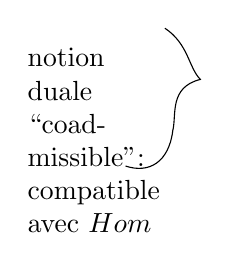
\begin{tikzpicture}[x=1cm,y=1cm]
\node[anchor=north west,text width=1.7cm,inner sep=0pt] at (0,0) {notion duale ``coadmissible'': compatible avec $\operatorname{Hom}$};
\handwritten{\draw (1.75,.25) .. controls (2.05,.05) and (2.05,-.25) .. (2.2,-.4) .. controls (1.8,-.5) and (1.9,-.85) .. (1.85,-1.05) .. controls (1.8,-1.45) and (1.55,-1.6) .. (1.25,-1.5);}
\end{tikzpicture}}}
\[
P\otimes_o F(X)\handwritten{\unsure{\text{---}|\longrightarrow}}F(P\otimes_o X)
\]
est un isomorphisme. Si $C$ est une catégorie de Deuring, alors il suffit de poser cette condition pour un objet fixé $X$ de $C$, et pour $o=\operatorname{End}_C(X)$, $P$ un module $\handwritten{\in}\uline{P}(\handwritten{o/A})=$ catégorie des $o$-modules à droite qui sont localement sur $S=\operatorname{Spec}(A)$ libres de rang $1$. Dans ce cas, la catégorie des foncteurs $F$ en question est équivalente, par
\margin{\handwritten{il suffit que $C$ admette $X$ \deleted{\unsure{comme|un}} ``générateur strict'' i.e. tt objet de $C$ de la forme $P\otimes_o X$, et que avec $P$ projectif de type fini, alors équiv. $\uline{P}\longmapsto P\otimes_o X$ (sur ss-cat $\unsure{\mathbb{P}(o)X|P(o)X}$) (pour $P\otimes_o X$ \unsure{existe})}}
\margin{\handwritten{$P\otimes_o X\overset{\sim}{\longrightarrow}\operatorname{Hom}_o(\check P,X)$}}
\[
F\handwritten{\longmapsto}F(X)\ :\ \uline{\operatorname{Hom}}_{A\text{-}\mathrm{adm}}(C,C')\handwritten{\hookrightarrow}\operatorname{Mod}(o,C'),
\]
à la catégorie des objets \inserted{$X'$} de $C'$ avec opération de $o$\inserted{$A$-linéaire de}, tels que $P\otimes_o X'$ exist dans $C'$ pour tout $P\handwritten{\in}\operatorname{ob}\uline{P}(o/A)$. En tous cas, la catégorie des foncteurs admissibles de $C$ dans $C'$ est $A$-linéaire.

\inserted{Soit}
\[
\deleted{\text{Soit}}\quad C(1)=\uline{\operatorname{Hom}}_{A\deleted{\text{-}\mathrm{adm}}\inserted{\handwritten{\mathrm{coadm}}}}(C^{\handwritten{\unsure{o|0|\circ}}},\operatorname{Mod}(A)),
\]
on a alors un foncteur pleinement fidèle canonique
\[
C\handwritten{\xrightarrow{i}}C(1)
\]
associant à tout objet $X$ de $C$ le foncteur $Y\handwritten{\longmapsto}\operatorname{Hom}_{\mathbb{C}}(Y,X)$ qu'il représente. \handwritten{Si $X$ est un objet de $C$ tel que tout objet \inserted{$Y$} de $C$ s'écrit sous la forme $P\otimes_o X$, avec $P$ un $o$-module à droite projectif de type fini $(o=\operatorname{End}_C(\unsure{X^{\prime}|X}))$.}
% archive sheet number: 58


\scanpage{62}
\mspage{\handwritten{- 34 -}}
La fonction égale à $\handwritten{f}$ dans $A$, à $\handwritten{g}$ dans $B$, est alors holomorphe dans $A\handwritten{\cup}B$ ; on dit que c'est un \uline{prolongement analytique} de $\handwritten{f}$ (ou de $\handwritten{g}$) à $A\handwritten{\cup}B$.

Le th.1 entraîne le résultat plus général suivant :

PROPOSITION 1.- \uline{Soit} $(A_{\handwritten{\alpha}})$ \uline{une famille de domaines dans} $K^p$, \uline{telsque}, \uline{pour tout couple d'indices} $\handwritten{\alpha,\beta}$, $A_{\handwritten{\alpha}}\handwritten{\cap}A_{\handwritten{\beta}}$ \uline{soit vide ou soit un domaine. Pour tout indice} $\handwritten{\alpha}$, \uline{soit} $\handwritten{f_\alpha}$ \uline{une fonction à valeurs dans} $E$, \uline{définie et holomorphe dans} $A_{\handwritten{\alpha}}$ ; \uline{on suppose que pour tout couple d'indices} $\handwritten{\alpha,\beta}$ \uline{tel que} $A_{\handwritten{\alpha}}\handwritten{\cap}A_{\handwritten{\beta}}\handwritten{\neq\varnothing}$, \uline{il existe un ensemble ouvert non vide contenu dans} $A_{\handwritten{\alpha}}\handwritten{\cap}A_{\handwritten{\beta}}$ \uline{et dans lequel} $\handwritten{f_\alpha(x)=f_\beta(x)}$. \uline{Dans ces conditions, il existe une.fonction} $\handwritten{f}$, \uline{holomorphe dans} $A=\handwritten{\bigcup_\alpha}A_{\handwritten{\alpha}}$, \uline{et telle que} $\handwritten{f(x)=f_\alpha(x)}$ \uline{pour tout} $\handwritten{x\in}A_{\handwritten{\alpha}}$ \uline{et tout} $\handwritten{\alpha}$.

En effet, pour tout $\handwritten{x\in}A$, les valeurs de $\handwritten{f_\alpha(x)}$ sont les mêmes pour tout $\handwritten{\alpha}$ tel que $\handwritten{x\in}A_{\handwritten{\alpha}}$, en vertu du th.1.

\uline{\handwritten{2}}.\quad \uline{Domaines d'existence ma\handwritten{-}ximaux}.\quad \uline{Points singuliers}.

Soit $A$ un domaine dans $K^p$, et $\handwritten{f}$ une fonction holomorphe dans $A$. Considérons l'ensemble $\handwritten{\mathscr{M}}$ des fonctions holomorphes définies dans un domaine contenant $A$, et \uline{prolongeant} $\handwritten{f}$ ; il est immédiat que $\handwritten{\mathscr{M}}$, ordonné par la relation ``$\handwritten{g}$ est une restriction de $\handwritten{h}$'' est \uline{inductif} ; en vertu du th. de Zorn, il admet donc au moins un élément maximal $\handwritten{f_{\unsure{0|o}}}$ ; \margin{\unsure{i}}\unsure{.} on dit que $\handwritten{f_{0}}$ est un \uline{prolongement analytique maximal} de $\handwritten{f}$, et que le domaine $A_{\handwritten{0}}$ où est définie $\handwritten{f_{0}}$ est un \uline{domaine d'existence maximal} pour un prolongement analytique de $\handwritten{f}$ (ou par abus de langage, pour $\handwritten{f}$ elle-même).

Si $A_{\handwritten{0}}$ est un domaine d'existence maximal pour $\handwritten{f}$, il résulte aussitôt du th.1 que le prolongement maximal de $\handwritten{f}$ dans $A_{\handwritten{0}}$ est \uline{unique}. Si $A_{\handwritten{0}}=K^p$ il n'y a qu'un seul domaine d'existence maximal pour $\handwritten{f}$,
% archive sheet number: 61


\scanpage{63}
de $C$ est de la forme $P\otimes_o X$ $(o=\operatorname{End}(X))$, avec $\unsure{P|\mathbb{P}}$ projectif de t.f. sur $o$) alors la condition que les produits tensoriels \unsure{soient} \unsure{raisonnables} équivaut à celle que \deleted{\unsure{les produits}} les $P\otimes_o X$ soient \unsure{stricts|stricte}, et implique que $\mathcal{C}$ est équivalente à une sous-catégorie pleine de $\mathbb{P}_d(o)$ ($o$-modules \inserted{à droite} projectifs de t.f.) \deleted{sur $o$ \unsure{soient}} \unsure{contenant} l'objet $\unsure{\uline{1}|1}$ (et inversement\unsure{?}). Mais la condition de \unsure{plénitude} est automatiquement satisfaite.
\margin{\unsure{?}}

D'autre part, \deleted{dans}\inserted{pour} catégorie \deleted{\unsure{finie}} $C$ jolie, considérant \deleted{\unsure{pour tt objet} $X$ de $C$ les \unsure{ss}}\inserted{les sous-catégories ``strictes''} monogènes'' de $C$, celles-ci font une suite croissante \inserted{de sous-catégories pleines}, et $C$ en est la limite inductive.

\[
\begin{aligned}
&\text{Catégorie }\deleted{\text{\unsure{g}}}\ A\text{-linéaire }\deleted{\text{\illegible{1}}}\text{jolie}\ \Longleftrightarrow\ \text{limite inductive de}\\
&\qquad\qquad\qquad\text{sous-catégories pleines,}\\
&\qquad\qquad\qquad\text{équivalentes}\ \inserted{\text{chacune}}\ \text{à}\ \deleted{\text{\unsure{une}}}\ \text{ss}\\
&\qquad\qquad\qquad\text{catégorie d'un }\mathbb{P}_{\unsure{a|d}}(o),\\
&\qquad\qquad\qquad\text{contenant l'\unsure{élément} }o,
\end{aligned}
\]
\margin{(}
% archive sheet number: 62


\scanpage{64}
\mspage{\handwritten{- 33 -}}
l'amplitude de $z$ comprise entre $0$ et $2\handwritten{\pi}$, $B$ est l'ensemble des $z\handwritten{\neq}0$ tels que $\handwritten{\frac{\pi}{3}<\theta'<\frac{5\pi}{3}}$. L'ensemble ouvert $A\handwritten{\cap}B$ est non connex ses deux composantes connexes $H$ et $H'$ étant respectivement défini par $\handwritten{-\frac{2\pi}{3}<\theta<-\frac{\pi}{3}}$ et $\handwritten{\frac{\pi}{3}<\theta<\frac{2\pi}{3}}$. Soit $f(z)=\handwritten{\sqrt{|z|}}\,e^{i\handwritten{\theta}/2}$ dans $A$, $g(z)=\handwritten{\sqrt{|z|}}\,e^{i(\handwritten{\theta'}-2\handwritten{\pi})/2}$ dans $B$ ; on a $(f(z))^{\handwritten{2}}=z$ dans $A$ et $(g(z))^{\handwritten{2}}=z$ dans $B$, et par suite, comme $f$ et $g$ sont continues, ce sont des fonctions holomorphes dans $A$ et $B$ respectivement (chap.I, \handwritten{\S}\,2, th.1). Mais dans $H$, on a $\handwritten{\theta'}=2\handwritten{\pi}+\handwritten{\theta}$, d'où $f(z)=g(z)$ et dans $H$, $\handwritten{\theta'=\theta}$, d'où $f(z)=-g(z)$.

\handwritten{2)} Lorsque $K=\handwritten{C}$, au lieu de supposer que $\handwritten{f(x)=g(x)}$ dans un ens% right edge clips the rest of this line; no em survives
ble ouvert non vide $U\handwritten{\subset}A\handwritten{\cap}B$, il suffit de supposer que $\handwritten{f(x)=g(x)}$ dans l'intersection d'un tel ensemble $U$ et d'une variét\unsure{é} linéaire réelle $V$ définie par $p$ équations de la forme $\handwritten{\unsure{\mathfrak{I}|\mathscr{I}|\mathscr{J}}}(z_k)=\handwritten{\beta}_k$ $(1\handwritten{\leq}k\handwritten{\leq}p)$, $U\handwritten{\cap}V$ étant supposé non vide. En effet, si $\handwritten{a\in}U\handwritten{\cap}V$, les dérivées partielles de $\handwritten{h}$ au point $a$ sont égales respectivement aux dérivées partielles de mêmes indices de la restriction de $\handwritten{h}$ à $U\handwritten{\cap}V$ ; comme par hypothèse ces dernières sont toutes nulles, la série entière (par rapport aux $x_i-a_i$) égale à $\handwritten{h(x)}$ dans un polycylindre assez petit de centre $\handwritten{a}$, a tous ses coefficients nuls, ce qui montre que $\handwritten{f(x)=g(x)}$ dans un voisina\handwritten{-}ge de $\handwritten{a}$ par rapport à $A\handwritten{\cap}B$.

Si $K=\handwritten{R}$ ou $K=\handwritten{C}$, et $p=1$, il suffit de supposer que $\handwritten{f(x)=g(x\unsure{)}}$ dans une partie $M$ de $A\handwritten{\cap}B$ telle que l'intersection de $M$ et d'un vois\unsure{i}na\handwritten{-}ge compact $U\handwritten{\subset}A\handwritten{\cap}B$ d'un point de $A\handwritten{\cap}B$ soit un ensemble \uline{infini}. En effet, il existe alors un point $\handwritten{b\in}U$ adhérent à une suite de points distincts $(z_n)$ de $U$ tels que $\handwritten{h}(z_n)=0$ pour tout $n$ ; d'après le principe des zéros isolés, on a $\handwritten{h(x)}=0$ dans un voisinage de $\handwritten{b}$ contenu dans $A\handwritten{\cap}B$, et on conclut comme précédemment.
% archive sheet number: 63


\scanpage{81}
Localisation pour les variétés abéliennes.

1.\quad \inserted{Soit $A$ un anneau commutatif.} Soit $C$ une catégorie $A$-linéaire (pas nécessairement additive; les $\operatorname{Hom}$ sont munis de structures $A$-linéaires, les accouplements sont $A$- bilinéaires). Pour toute\deleted{\unsure{anneau $R$}} $A$-algèbre $A'$, soit $C_{A'}$ la catégorie ayant mêmes objets que $C$, et où les $\operatorname{Hom}$ sont
\[
\operatorname{Hom}_{C_{A'}}(X,Y)=\operatorname{Hom}_C(X,Y)\otimes_A A'.
\]
On trouve ainsi une\deleted{champ en}\inserted{catégorie fibrée \deleted{en}\inserted{\handwritten{\uline{$C$}}}} catégories $\unsure{\mathbb{R}|\mathbb{A}}$-linéaires sur le site annelé des schémas affines $\operatorname{Spec}(A')$ sur $S=\operatorname{Spec}(A)$. Elle n'est pratiquement jamais un champ sur ce gros site, même p\unsure{\deleted{i}o|\deleted{o}i}ur une topologie assez grossièr\unsure{\deleted{i}e|é|\deleted{e}i} comme la topologie de Zariski. Cependant, si on se restreint au petit site de Zariski \inserted{affine} de $S$ des ouverts affines de $S$, on a souvent un champ (pour la topologie de Zariski), \deleted{Ceci a des conséquences}\inserted{soit $\uline{C}$.} \handwritten{On dit alors que $C$ est \uline{localisable} \uline{sur} $A$.}
\margin{\handwritten{\uuline{$C$}}}

Supposons cette condition\deleted{s} satisfaite. On\inserted{\handwritten{n}} a des conséquences agréables, comme:

a)\quad So\unsure{\deleted{i}p|\deleted{p}i}t \deleted{$E$} $R$ une $A$-algèbre (pas néc. commutative), et $X$ un objet de $C$ muni d'une opération $\mathbb{R}$-linéaire de $R$. Alors pour tout $R$-module à d\unsure{\deleted{o}r|\deleted{r}o}oite $P$, qui est isomorphe localement sur $S$ à $R_{\unsure{d|a}}$, le produit tensoriel $P\otimes_R X$ dans $C$ existe, et \inserted{si $R\quad\operatorname{End}_C(X)$ est bijectif,} le foncteur
\[
P\qquad P\otimes_R X
\]
de la catégorie \inserted{$\uline{P}(R)$} des $R$-modules à droite localement isomorphes à $R$ sur $S$ dans la catégorie $C$ est pleinement fidèle, \handwritten{et son image essentielle \unsure{est} formée des $X'\in\operatorname{Ob}C$ qui sont ``localement isomorphes à $X$'' sur $A$.}

b)\quad Supposons que $C$ soit additive. Alors $\uline{C}$ est un champ en catégories additives $\mathbb{R}$-linéaires. Pour tout $X$, $R$ comme dessus, \deleted{et} et tout module à droite $P$ sur $R$ qui est localement sur $S$ libre de type fini, le produit tensoriel $\mathbb{P}\otimes_R X$ existe, et si $R\quad\operatorname{End}_C(X)$, le foncteur $\unsure{\deleted{P}|\mathbb{P}|\mathbb{R}}$
\[
P\qquad P\otimes_R X
\]
% archive sheet number: 80


\scanpage{82}
de la catégorie de ces modules vers $C$ est pleinement fidèle, et son image essentielle est formée des objets $X'$ de $C$ qui sont localement sur $S$ isomorphes à un objet de la forme $X^n$.

NB\quad La conclusion de b) est satisfaite si, au lieu de supposer $C$ localisable, on la suppose stable par facteurs directs (=karoubienne), et \deleted{en fait $P$} si on prend des $P$ projectifs de type fini sur $R$.

c)\quad Soit toujours $R$ une $A$-algèbre\unsure{ \inserted{de type fini},|, \inserted{de type fini}} et soit $\operatorname{Mod}\unsure{\deleted{f}(|(}R,C)$ la catégorie des objets de $R$ munis d'une opération $R$-linéaire. \unsure{\deleted{C}A|\deleted{A}C}'est une catégorie $A$-li\unsure{néé|né}aire, et \unsure{\deleted{d}l|\deleted{l}d}a catégorie fibrée des
\figure{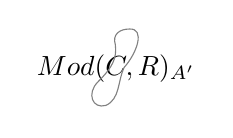
\begin{tikzpicture}[baseline=(m.base)]
\node (m) at (0,0) {$\operatorname{Mod}(\uuline{C},R)_{A'}$};
\handwritten{\draw[gray] (.17,.50) .. controls (.37,.51) and (.27,.20) .. (.10,.01) .. controls (.02,-.16) and (.05,-.39) .. (-.13,-.47) .. controls (-.30,-.52) and (-.38,-.32) .. (-.23,-.17) .. controls (-.04,.02) and (.01,.13) .. (-.01,.30) .. controls (-.05,.43) and (.04,.50) .. (.17,.50);}
\end{tikzpicture}}
(pour $A'$ \deleted{anneau} \deleted{affine d'un ouvert affine de $S=\operatorname{Spec}(A)$)}\inserted{une $A$-algèbre)} est équivalente à la catégorie fibrée des sections de $\uline{C}$ munis d'une opération de $R$\unsure{\deleted{n}.|n} \unsure{En|Bn} particulier, sa restriction au \deleted{site} petit site zariskien affine de $S$ \deleted{\unsure{site|sitd}} s'identifie à
\figure{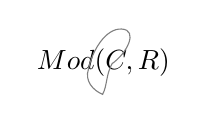
\begin{tikzpicture}[baseline=(m.base)]
\node (m) at (0,0) {$\operatorname{Mod}(\uline{C},R)$};
\handwritten{\draw[gray] (.23,.43) .. controls (.45,.42) and (.30,.12) .. (.11,-.01) .. controls (.03,-.16) and (.05,-.29) .. (-.01,-.40) .. controls (-.13,-.35) and (-.24,-.23) .. (-.19,-.08) .. controls (-.14,.16) and (.03,.44) .. (.23,.43);}
\end{tikzpicture}}
; c'est donc un champ si $\uline{C}$ en est un, donc $\operatorname{Mod}(R,\unsure{\deleted{C}|\mathbb{C}|\mathbb{A}})$ est localisable \inserted{s\unsure{\deleted{e}u|\deleted{u}e}r $S$} si $C$ l'est.

NB\quad Si $R$ est commutatif, $\operatorname{Mod}(R,C)$ est même $R$-linéaire. Notre raisonnement \uline{ne prouve pas} que \deleted{$C$ est} $\operatorname{Mod}(R,C)$ est local\deleted{\unsure{r|i}}isable sur $R$ i.e. sur $\operatorname{Spec}(R)$ (ce qui est plus fort que de dire qu'elle est localisable sur $S=\operatorname{Spec}(A)$).

d)\quad \deleted{Deux objets de $\unsure{X',Y|X;Y}$ de $C$ tels que sont dits} Si $C$ est localisable sur $A$, alors pour $A'$ \deleted{ouvert} anneau affine d'un ouvert affine \inserted{$U$} de $S$, $C_{A'}$ est localisable sur $A'$, et le champ associé sur $U$ s'identifie à la restriction d\unsure{\deleted{e}u|\deleted{u}e} champ $\uline{C}$ à $U$.

e)\quad Deux objets de $C$ sont dits apparentés (ou $A$-\unsure{\deleted{p}a|\deleted{a}p}pparentés) s'ils sont localement isomorphes sur $A$. \unsure{\deleted{D}C|\deleted{C}D}'est évidemment une relation d'équivalence, et la sous-catégorie pleine de $C$ formée des objets apparentés à un objet de $C$ est une catégorie \deleted{de} $A$-linéaire localisable sur $A$, et c'est une catégorie de Deuring,
% archive sheet number: 81


\scanpage{136}
\begin{flushright}1.4.68\end{flushright}
\margin{\handwritten{\unsure{4|V}}}

\uline{D I V E R S}

\uline{CANDIDATS}

.\quad TAFT

.\quad Scientifiques Russes

-\quad A la demande de M. MICHEL, revoir les dossiers de :

DASGUPTA

OKABAYASHI

ROCKMORE

SHIMA

SOMMER

YOKOO

\diagram{$\begin{array}{lll}
\text{-\quad Suggestion M. MICHEL\quad :} & ( & \text{polonais}\\
 & ) & \text{indiens}
\end{array}$}
% archive sheet number: 135


\scanpage{170}
Fonc\uline{teurs fibres motiviques, et gps fondame}% word cut off by torn right edge; no further letters survive
\uline{motiviques}.

À examiner :

0)\quad VA
\figure{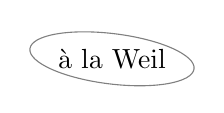
\begin{tikzpicture}[baseline=(w.base)]\node (w) at (0,0) {à la Weil};\draw[gray] (0,0) ellipse [x radius=1.05,y radius=.32,rotate=-7];\end{tikzpicture}}
\unsure{associées} aux motifs purs de poids impairs sur
\inserted{Conditions \unsure{de|\uline{de}|\deleted{de}} Hodge-Riemann\ldots}

\margin{OK\quad *}
\figure{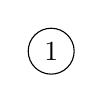
\begin{tikzpicture}\node[draw,circle,inner sep=3pt] {1};\end{tikzpicture}}
Extension \unsure{du|de} \unsure{groupe|groupes} \unsure{définie|définies|défini} par des \unsure{pts motiviques|places arithmétiques|places antiques}

Grou\uline{pe fondamental motivique}.

\figure{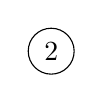
\begin{tikzpicture}\node[draw,circle,inner sep=3pt] {2};\end{tikzpicture}}
Relations avec le corps de classes

\margin{OK}
\figure{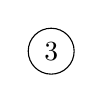
\begin{tikzpicture}\node[draw,circle,inner sep=3pt] {3};\end{tikzpicture}}
Cas du spectre d'un corps fini. Pts motiviques

parties à val. dans $\mathbb{R}$ ???

\margin{*}
4)\quad Rôle \unsure{du|des} \unsure{gpe|groupe|gps} \unsure{fondamental|fondamentaux} motivique pour la comparaison des réseaux canoniques
\diagram{$\left[\begin{array}{ll}
\text{dans Ch. de Hodge} & \left|\begin{array}{l}
\text{2 réseaux transcendant \unsure{pr.|prov.} \unsure{des|deux} places diff.}\\
\text{réseau transcendant et \unsure{réseau|réseaux} de Hodge}
\end{array}\right.\\[1em]
\text{dans Coh. $l$-adique} & \left|\text{2 réseaux transcendants}\right.
\end{array}\right]$}

5)\quad Relations \inserted{de 4} avec mes \unsure{notes|autres} \unsure{anciennes|anciens}

6)\quad \unsure{Fonction|Fonctions} $L$: équation fonctionnelle

\margin{OK}
7)\quad Structures \unsure{pratiques|positives|p-adiques}\ldots

\deleted{7}8)\quad Topologie à mettre sur $\mathbb{Z}$ \texttt{-{}-{}-{}-}

9)\quad Hyp. de Riemann \unsure{??}

\margin{Positivité à la Hodge en se ramenant à des questions de \uline{diviseurs} par éclatements, ou Variétés de drapeaux ??}
% archive sheet number: 169


\scanpage{171}
\mspage{(20)}
SYSTÈMES de RACINES\hfill Tribu n$^{\handwritten{o}}$ \unsure{\handwritten{59}|59}

de signe $+1$.

1) On pose $E=\unsure{\mathbb{I}|\Gamma|\mathbb{P}|L|\Pi}\handwritten{/}\unsure{\handwritten{3}|3}P$. C'est un $\uuline{F}_{\handwritten{3}}$-espace vectoriel de dimension \unsure{5|\handwritten{5}}. Montrer que le produit $(x,y)$ définit sur $E$ une forme bil. sym. non dégénérée. Montrer que deux éléments distincts de $R$ ont des images distinctes dans $E$.

2) On note $\operatorname{O}(E)$ le groupe orthogonal de $E$, muni de la forme bil. précédente. On a $\operatorname{O}(E)=\handwritten{\{\pm}1\handwritten{\}}\times\operatorname{SO}(E)$. La norme spinorielle définit un homomorphisme surjectif $\operatorname{SO}(E)\handwritten{\longrightarrow\{\pm}1\handwritten{\}}$ dont le noyau est noté $\operatorname{SO}^{\handwritten{+}}(E)$. Le groupe $\operatorname{SO}^{\handwritten{+}}(E)$ est simple, (d'ordre \unsure{25 920|\handwritten{25 920}}) ; le quotient $\operatorname{O}(E)/\operatorname{SO}^{\handwritten{+}}(E)$ est de type $(2,2)$. En déduire que $\operatorname{O}(E)$ contient un sous-groupe $\handwritten{\Omega}(E)$ d'indice 2 distinct de $\operatorname{SO}(E)$ et ne contenant pas $-1$ ; montrer que ce sous-groupe est unique.

3) Tout élément de $\operatorname{Aut}(R)$ définit par passage au quotient un élément de $\operatorname{O}(E)$. Montrer, (en comparant les ordres), que l'on obtient ainsi un isomorphisme de $\operatorname{Aut}(R)$ sur $\operatorname{O}(E)$ ; l'image de $W(R)$ par cet isomorphisme est $\handwritten{\Omega}(E)$, celle de $W^{\handwritten{+}}(R)$ est $\operatorname{SO}^{\handwritten{+}}(E)$.

(Ainsi, $W(R)$ est extension d'un groupe à deux éléments \unsure{oar|par} le groupe simple d'ordre 25 920).

F) Groupe de Weyl $W$ de $E_{\unsure{\handwritten{7}|7}}$.

Soient $Q$ le réseau radiciel, $P$ celui des poids. On a $2P\handwritten{\subset}Q$. Posons $E=Q\handwritten{/}2P$. La forme bilinéaire $(x\ y)$ définit, par passage au quotient, une forme bilinéaire sur le $F_{\unsure{\handwritten{2}|2}}$-espace vectoriel $E$, (noter que $(Q\mid 2P)\handwritten{\subset}2Z$). Montrer que cette forme est non dégénérée et alternée, (noter que $\dim(E)=\unsure{\handwritten{6}|6}$). En déduire un homomorphisme $W\handwritten{\longrightarrow}\operatorname{Sp}(E)=\operatorname{Sp}(3,F_{\handwritten{2}})$.

Montrer que la suite
\[
\text{(s)}\qquad 1\handwritten{\longrightarrow}(1,-1)\handwritten{\longrightarrow}W\handwritten{\longrightarrow}\operatorname{Sp}(3,F_{\handwritten{2}})\handwritten{\longrightarrow}1
\]
est exacte, (on peut utiliser le fait que $\operatorname{Sp}(3,F_{\handwritten{2}})$ est d'ordre $2^{\unsure{\handwritten{9}|9}}.3^{\unsure{\handwritten{4}|4}}.5.7$ ; cf. Alg. IX).

Montrer que le sous-groupe $W^{\handwritten{+}}$ formé des éléments de déterminant 1 de $W$ se projette isomorphiquement sur $\operatorname{Sp}(3,F_{\handwritten{2}})$, (noter que ce sous-groupe ne contient pas $-1$).

Donner une seconde démonstration de (s) en utilisant la structure de $W(E_{\unsure{\handwritten{8}|8}})$ et l'isomorphisme $\operatorname{Sp}(3,F_{\handwritten{2}})\handwritten{\longrightarrow}\uline{\operatorname{O}}(7,F_{\handwritten{2}})$.
% archive sheet number: 170


\scanpage{181}
% The printed list is upside down in the supplied scan; reading order follows the upright list.
\diagram{$\begin{array}{llllll}
\text{0170} & \text{TAULELLE} & \text{VERONIQUE} & \text{2740730007019} & \text{930728S} & \text{2A2} \\
\text{0171} & \text{TIGNY} & \text{SANDRINE} & \text{2710769383109} & \text{900477U} & \text{2A2} \\
\text{0172} & \text{TOURIERE} & \text{SOPHIE} & \text{2740434172243} & \text{942009J} & \text{2A2} \\
\text{0173} & \text{TRIAIRE} & \text{AGNES} & \text{2720934111012} & \text{910300B} & \text{2A2} \\
\text{0174} & \text{TRIAIRE} & \text{FRANCOISE} & \text{2720934111013} & \text{910299A} & \text{2A2} \\
\text{0175} & \text{TUFFERY} & \text{ISABELLE} & \text{2700534172087} & \text{931766V} & \text{2A2} \\
\text{0176} & \text{VALMALETTE} & \text{SOPHIE} & \text{2710778551110} & \text{941607X} & \text{2A2} \\
\text{0177} & \text{VEDEL} & \text{KARINE} & \text{2710643157065} & \text{911395S} & \text{2A2} \\
\text{0178} & \text{VERGER} & \text{ESTELLE} & \text{2730234172047} & \text{920133V} & \text{2A2} \\
\text{0179} & \text{VICART} & \text{DAVID} & \text{1720362119173} & \text{910910P} & \text{2A2} \\
\text{0180} & \text{VIDAL} & \text{CAROLE} & \text{2720434172236} & \text{910273X} & \text{2A2} \\
\text{0181} & \text{VILLAR} & \text{MAXIME} & \text{1700934032119} & \text{900007H} & \text{2A2} \\
\text{0182} & \text{WINTREBERT} & \text{CLAIRE} & \text{2730334172023} & \text{923054V} & \text{2A2} \\
\text{0183} & \text{WOUTERS} & \text{FREDERIQUE} & \text{2721059350782} & \text{920453T} & \text{2A2} \\
\end{array}$}

*****\quad FIN\quad LISTE\quad *****
% archive sheet number: 180


\scanpage{188}
\handwritten{\mspage{70}}
that there exists $n_{\handwritten{\unsure{o|0}}}(K)$ such that at $n\ \handwritten{\mathrm{m}}\ n_{\handwritten{o}}(K)$
\[
\handwritten{H^i(V,K[nE])=0\qquad i=1,2,\ldots}
\]

From the exact sequence
\[
\handwritten{H^i(V,O_V(-E_\varphi)[nE])\longrightarrow H^i(V,O_V[nE])\longrightarrow H^i(V,K[nE])}
\]
at $n\geq n_{\handwritten{o}}(K)$, $i=1,2,\ldots$ we obtain:
\[
\handwritten{\dim H^i(V,O_V[nE])\leq\dim H^i(V,O_V(-E_\varphi)[nE]).}
\]

Since
\[
\handwritten{O_V(-E_\varphi)\cong O_V[-E],}
\]
then
\[
\handwritten{O_V(-E_\varphi)[nE]\cong O_V[-E][nE]\cong O_V[(n-1)E].}
\]

Therefore, at $n\geq n_{\handwritten{o}}(K)$, $i=1,2,\ldots$
\[
\handwritten{\dim H^i(V,O_V[nE])\leq\dim H^i(V,O_V[[n-1]E]).}
\]

Evidently, there exists such $n'$ that, at $n\geq n'$
% archive sheet number: 187


\cotefile{26}
\scanpage{2}

\begin{flushright}
$\underline{\overline{\mathrm{V}}}$\qquad Plan\\
\unsure{Notations}
\end{flushright}
% archive sheet number: 1


\clearpage
\scanpage{3}

A) \uline{Descente et passage au quotient}

\S\,1\quad Descente fidèlement plate

\S\,2\quad \deleted{Passage \unsure{au|aux} quoti\unsure{ent|.} \unsure{Généralités} sur les foncteurs sur} \inserted{Topologies sur $(\mathrm{Sch})_{/S}$. Propriétés générales des foncteurs sur $(\mathrm{Sch})_{/S}$.} \margin{[Intervertir \uline{1} et \uline{2} ??]}
\par\noindent\hfill\deleted{$(\mathrm{Sch})_{/S}$}

\S\,3\quad Passage au quotient plat.

\S\,4\quad Descente non plate\quad [\unsure{Application|Applications|Applicat.} : \unsure{Ram.|Rau.|Rem.} Samuel \unsure{généralisé} \ldots

\inserted{Appl. à platitude d'une adh. \unsure{schématique} et lemme de \deleted{\unsure{H}}Hironaka.}

\S\,5\quad Passage au quotient non plat. [\unsure{Passage} \unsure{aux|au} \unsure{quots|quot.} en gén]

\S\,6\quad Descente de schémas, relatifs étales, ----

[\unsure{Év\textsuperscript{t}|Éu\textsuperscript{t}}. descente des \deleted{\unsure{morphismes}}\inserted{faisceaux} étales ?? \ldots]

B) \deleted{\uline{Propriétés générales des foncteurs sur} $(\mathrm{Sch})_{/S}$.}

\figure{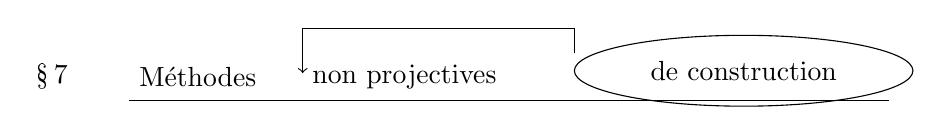
\begin{tikzpicture}[x=1cm,y=1cm]
\node[anchor=west] at (-1.3,0) {\deleted{\S\,7}};
\node[anchor=west] at (0,0) {Méthodes};
\node[anchor=west] at (2.2,0) {non projectives};
\node (construction) at (7.8,.08) {\inserted{de construction}};
\draw (construction.center) ellipse (2.15cm and .45cm);
\draw[->] (5.65,.3) -- (5.65,.62) -- (2.2,.62) -- (2.2,.05);
\draw (0,-.3) -- (9.65,-.3);
\end{tikzpicture}}

\figure{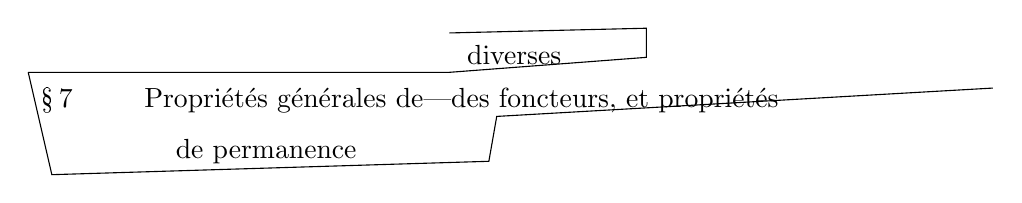
\begin{tikzpicture}[x=1cm,y=1cm]
\node[anchor=west] at (-1.3,0) {\deleted{\S\,7}};
\node[anchor=west] at (0,0) {\deleted{Propriétés générales \unsure{de|des} \unsure{foncteurs}, et propriétés}};
\node[anchor=west] at (.4,-.65) {\deleted{de permanence}};
\node[anchor=west] at (4.1,.58) {\deleted{\inserted{\unsure{diverses}}}};
\draw (-1.35,.36) -- (4.0,.36) -- (6.5,.55) -- (6.5,.92) -- (4.0,.86);
\draw (-1.35,.36) -- (-1.05,-.94) -- (4.5,-.77) -- (4.6,-.2) -- (10.9,.16);
\end{tikzpicture}}

\S\,7\quad \uline{Proreprésentabilité}: (et variantes).

\tikz[baseline=(p.base),remember picture]{\node[inner sep=1pt] (p) {\S\,\deleted{\unsure{8}}9};}\quad
\uline{Invariants différentiels} \deleted{\unsure{de|du} \unsure{div.}} \inserted{\uline{\unsure{tangts|tang.} et normaux}}

\tikz[baseline=(q10.base)]{\node[inner sep=1pt] (q10) {\S\,10};\draw (q10.center) ellipse (1.25em and .9em);}\quad
\margin{\fbox{Après \S\,12 ??}}Propriétés générales de foncteurs, \uline{propriétés de permanence}
\margin{$\left\{\begin{gathered}\text{Foncteurs \uline{excellent} sur S}\\ \text{morphismes excellent}\\ \text{??}\end{gathered}\right.$}

\tikz[baseline=(q11.base),remember picture]{\node[inner sep=1pt] (q11) {\S\,\deleted{\unsure{10|11}}11};\draw (q11.center) ellipse (1.65em and .9em);}\quad
\margin{\tikz[remember picture]{\node[draw,inner sep=2pt] (m11) {\parbox{.90\marginparwidth}{\raggedright Commun au \unsure{par.} \unsure{20|2e|éd} ? Cas Greenberg ?}};}}
Représentabilités ``élémentaires'' du type $\prod_{\deleted{X}Y/S}X/Y$.

\inserted{cf SGAD $\underline{\overline{\mathrm{VIII}}}$ 6 et $\underline{\overline{\mathrm{XI}}}$ 6.8.}

\tikz[baseline=(r.base),remember picture]{\node[draw,rounded corners,inner sep=1pt] (r) {\S\,8\deleted{\unsure{1|11}}};}
\quad Construction de Modules cohérents
\figure{\begin{tikzpicture}[remember picture,overlay]\draw[->] (r.north west) to[out=125,in=190] (p.north);\draw (q11.east) -- (m11.west);\end{tikzpicture}}

\S\,12\quad \deleted{\unsure{Représentabilité}}\inserted{Foncteurs} \unsure{repr.} par morphismes \inserted{\uline{\unsure{séparés|xprés}}} loc. pr. \unsure{f|fi}

\S\,13\quad Applications : des \unsure{th\textsuperscript{es}|th\textsuperscript{s}} \deleted{de} représentabilité relatifs. (y compris \unsure{(}pour les es foncteurs étales\ldots\unsure{,|)}

% archive sheet number: 2


\clearpage
\scanpage{4}
\mspage{\unsure{\handwritten{(32}|(32}}

% One long pencil cancellation descends from the right of the opening lines
% to the left of the last paragraph. Local obliterations are nested below.
\newsavebox{\coteFourTypescript}
\begin{lrbox}{\coteFourTypescript}
\begin{minipage}[t]{.96\linewidth}
\llap{\handwritten{\tikz[baseline]{\draw[thin] (0,0) .. controls (.16,.2) and (.34,.37) .. (.43,.17);}}}Considérant la restriction de $\handwritten{\varphi}$ à la sous-catégorie pleine de $\overset{\handwritten{\sim}}{\mathrm{X}_{\text{ét}}}$ formée des ouverts de ce topos, ou ce qui revient au même \handwritten{(6.1.)} des ouverts $\mathrm U$ de $\mathrm X$, on trouve une application
\[
\handwritten{\varphi_{0}}:\handwritten{\mathcal U}(\mathrm X)\mathrel{\mbox{-}\mkern-2mu\mbox{-}\mkern-3mu\handwritten{\to}}\handwritten{\bigl\{}0,1\handwritten{\bigr\}}
\]
commutant aux sup quelconques et aux inf finis. (On note que pour $\mathrm U\handwritten{\in\mathcal U}(\mathrm X)$, $\handwritten{\varphi}(\mathrm U)$ est vide ou réduit un point, et on prend $\handwritten{\varphi_{0}}(\mathrm U)=0$ ou $1$ suivant qu'on est dans l'un ou l'autre cas).

On voit facilement \deleted{(\illegible{1}\unsure{)}}, grâce au fait que tout fermé irréductible de $\mathrm X$ a un point génerique et un seul, que $\handwritten{\varphi_{0}}$ est defini à l'aide d'un \deleted{\unsure{e|x}} unique $\mathrm x\handwritten{\in}\mathrm X$, par la condition
\[
\begin{aligned}
&\handwritten{\varphi_{0}}(\mathrm U)=1\qquad\text{sss}\qquad \mathrm x\handwritten{\mathrm E}\mathrm U\,,\\
\text{i.e.}\qquad &\handwritten{\varphi}(\mathrm U)\ne\varnothing\quad \mathrel{\handwritten{\Leftarrow}\mkern-7mu=\mkern-7mu\handwritten{\Rightarrow}}\quad \mathrm x\handwritten{\in}\mathrm U\,.
\end{aligned}
\]
Soit $\mathrm F\handwritten{\in}\operatorname{Ob}\overset{\handwritten{\sim}}{\mathrm X_{\text{ét}}}$, alors l'image de $\mathrm F$ dans le faisceau final $\mathrm X$ est un ouvert; et comme
\[
\handwritten{\varphi}(\mathrm F)\mathrel{\mbox{-}\mkern-2mu\mbox{-}\mkern-3mu\handwritten{\to}}\handwritten{\varphi}(\mathrm U)
\]
est surj\makebox[0pt][l]{\raisebox{.95ex}{\handwritten{\scriptsize\unsure{''}}}}ectif, on voit que $\handwritten{\varphi}(\mathrm F)\ne\varnothing$ sss $\handwritten{\varphi}(\mathrm U)\ne\varnothing$ i.e. sss $\mathrm x\handwritten{\in}\mathrm U$. Soit alors $\mathrm C_{\handwritten{\varphi}}$ la catégorie des couples $(\mathrm X',\handwritten{\xi})$ où $\mathrm X'\handwritten{\in}\operatorname{Ob}\mathrm X_{\text{ét}}$, et $\handwritten{\xi\in\varphi}(\mathrm X')$. On a signalé dans \handwritten{7.9.1.} que $\mathrm C_{\handwritten{\varphi}}^{\handwritten{\unsure{o|0|\circ}}}$ est pseudo-filtrante connexe. De plus grâce à \handwritten{7.9.2.} et à ce qui précéde appliqué à $\mathrm X'$ au lieu de $\mathrm X$, si $(\mathrm X',\handwritten{\xi})\handwritten{\in}\operatorname{Ob}\mathrm X_{\text{ét.}}$, il lui est\unsure{:} associé un unique point $\mathrm x'\handwritten{\in}\mathrm X'$, tel que pour un morphisme étale $\mathrm X''\mathrel{\mbox{-}\mkern-2mu\mbox{-}\mkern-2mu\mbox{-}\mkern-3mu\handwritten{\to}}\mathrm X'$, $\handwritten{\xi}$ est dans l'image de $\handwritten{\varphi}(\mathrm X'')\mathrel{\mbox{-}\mkern-2mu\mbox{-}\mkern-3mu\handwritten{\to}}\handwritten{\varphi}(\mathrm X')$ sss $\mathrm x'$ est dans celle de $\mathrm X''$. On conclut de ceci que le\deleted{\unsure{s}} préschéma\deleted{\unsure{s}} $\underset{\handwritten{\longleftarrow}}{\lim}$ des $\mathrm X'$ suivant la catégorie $\mathrm C$ des $(\mathrm X',\handwritten{\xi})$ existe et est un localisé strict $\mathrm Z$ de $\mathrm X$, correspondant donc à un point géométrique $\handwritten{\xi}$ et un foncteur \deleted{\unsure{l|b}}fibre $\handwritten{{\unsure{\bar{\mathcal E}|\mathcal E|\bar{\varepsilon}|\varepsilon}}_{\xi}}$.
\end{minipage}
\end{lrbox}
\noindent\begin{tikzpicture}
\node[inner sep=0pt,outer sep=0pt] (body) {\begingroup\renewcommand{\ULthickness}{0pt}\deleted{\usebox{\coteFourTypescript}}\endgroup};
\draw[gray,thin] (body.south west) ++(.37\linewidth,.5em) -- ([xshift=-.31\linewidth,yshift=-2.6em]body.north east);
\end{tikzpicture}
% archive sheet number: 3


\clearpage
\scanpage{5}
\figure{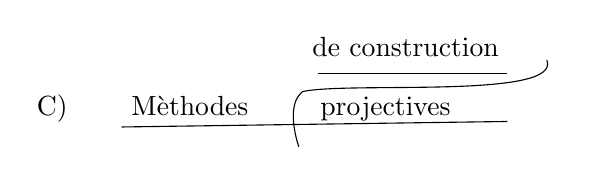
\begin{tikzpicture}[every node/.style={anchor=base west}]
\node at (0,0) {C)};
\node at (1.2,0) {Mèthodes};\node at (3.6,0) {projectives};
\node at (3.5,.75) {\inserted{de construction}};
\draw (1.2,-.15)--(6.1,-.08);\draw (3.7,.53)--(6.1,.53);
\draw (6.6,.7)..controls (6.8,.2) and (4.1,.43)..(3.5,.3)..controls (3.3,.15) and (3.4,-.25)..(3.45,-.4);
\end{tikzpicture}}

\S\,14\quad Familles limitées.

\figure{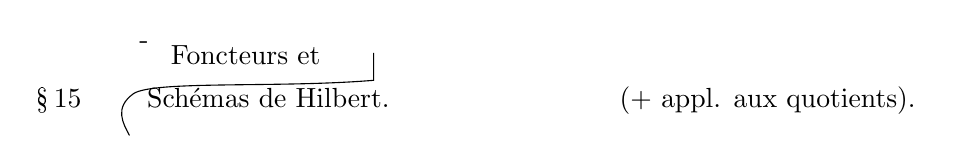
\begin{tikzpicture}[every node/.style={anchor=base west}]
\node at (0,0) {\S\,15};\node at (1.4,0) {Schémas de Hilbert.};\node at (7.4,0) {(+ appl. aux quotients).};
\node at (1.7,.55) {\inserted{Foncteurs et}};\node at (1.3,.75) {\unsure{-}};
\draw (4.4,.7)--(4.4,.35)..controls (3.2,.25) and (1.6,.35)..(1.35,.18)..controls (1.1,0) and (1.22,-.2)..(1.3,-.35);
\end{tikzpicture}}

\figure{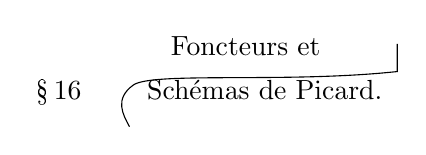
\begin{tikzpicture}[every node/.style={anchor=base west}]
\node at (0,0) {\S\,16};\node at (1.4,0) {Schémas de Picard.};
\node at (1.7,.55) {\inserted{Foncteurs et}};
\draw (4.7,.7)--(4.7,.35)..controls (3.3,.2) and (1.6,.35)..(1.35,.18)..controls (1.1,0) and (1.22,-.2)..(1.3,-.35);
\end{tikzpicture}}
\margin{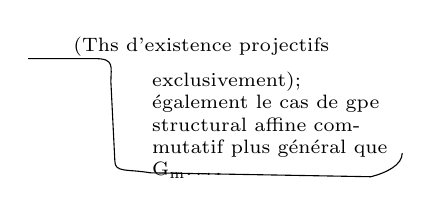
\begin{tikzpicture}[every node/.style={anchor=north west,font=\scriptsize,align=left}]
\node[text width=4cm] at (0,0) {(Ths d'existence projectifs};
\node[text width=3.2cm] at (1,-.45) {exclusivement\deleted{\unsure{)}}; également le cas de gpe structural affine commutatif plus général que $\mathrm G_{\mathrm m}$\ldots.};
\draw (-.45,-.4)--(.4,-.4)..controls (.65,-.4) and (.6,-.5)..(.6,-.7)--(.65,-1.7)..controls (.65,-1.85) and (.8,-1.8)..(1.1,-1.85)--(3.9,-1.9)..controls (4.1,-1.85) and (4.3,-1.75)..(4.3,-1.6);
\end{tikzpicture}}

\S\,17\quad Variantes de Picard.

\S\,1\deleted{\unsure{7}}8\quad Applications aux courbes

\S\,1\deleted{\unsure{8}}\unsure{9|8}\quad Formalisme des normes

\S\,\deleted{\unsure{19}}20\quad Invariants multiprojectifs de Mumford.

\figure{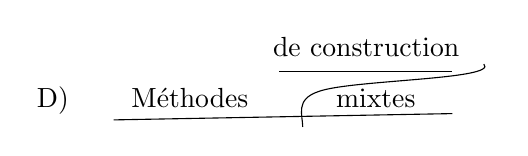
\begin{tikzpicture}[every node/.style={anchor=base west}]
\node at (0,0) {D)};\node at (1.2,0) {Méthodes};\node at (3.8,0) {mixtes};
\node at (3,.65) {\inserted{de construction}};
\draw (1.1,-.16)--(5.4,-.08);\draw (3.2,.45)--(5.4,.45);
\draw (5.8,.55)..controls (6,.35) and (4.1,.35)..(3.7,.2)..controls (3.4,.1) and (3.5,-.1)..(3.5,-.25);
\end{tikzpicture}}

\S\,2\deleted{0}1\quad Cas de représentabilité de $\mathrm P\underline{\mathrm{ic}}$, $\mathrm P\underline{\mathrm i\unsure{\mathrm c|\mathrm e}}^{\unsure{0|o|\circ}}$, $\unsure{-|\deleted{\mathrm P}}\mathrm P\underline{\mathrm{ic}}_{X}^{\tau}$ \ldots

(y compris le cas de Mumford utilisant \S\,\deleted{\unsure{19}}20).

\S\,21\quad Cas de représentabilité des foncteurs $\prod_{\deleted{X}Y/S}X/Y$ etc.

(\unsure{ths|Ths} du type Matsumura).

\noindent\rule{\linewidth}{.3pt}

NB.\quad On suppose \unsure{connues|connus} toutes les \unsure{gén.} fonctorielles (topologies, descente faisceaux, \unsure{quotients|quotient}) ; à rappeler au besoin dans $\unsure{0|O}_{\underline{\overline{\mathrm V}}}$.

\noindent\rule{\linewidth}{.3pt}

\uline{Manquent} :

\figure{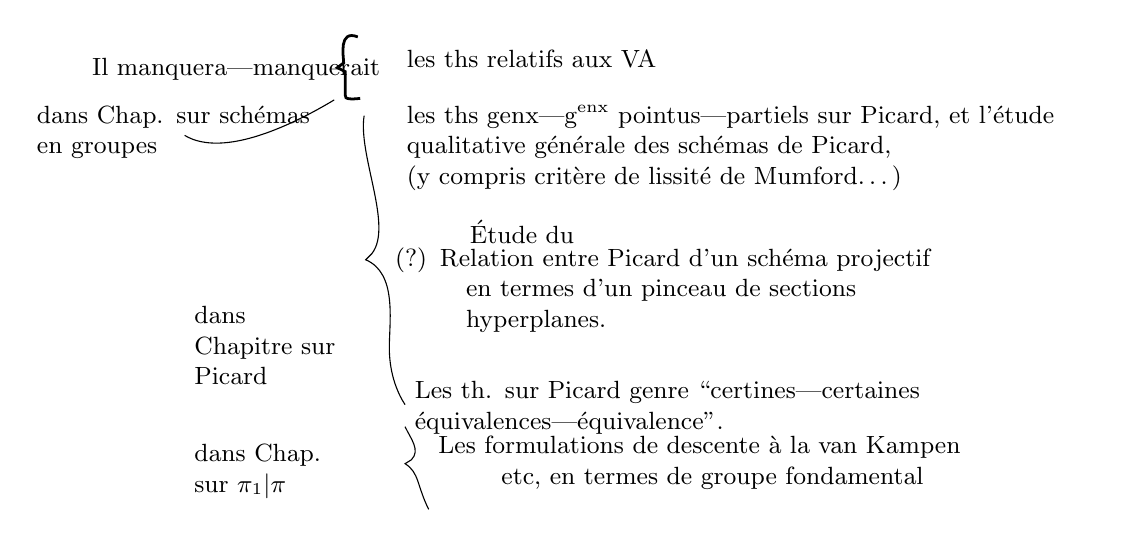
\begin{tikzpicture}[every node/.style={anchor=north west,align=left,font=\small}]
\node at (.7,0) {\deleted{Il \unsure{manquera|manquerait}}};
\node[text width=3.6cm] at (0,-.6) {dans Chap. sur schémas\\en groupes};
\node at (4.7,.1) {les ths relatifs aux VA};
\node[text width=8.3cm] at (4.7,-.6) {les ths \unsure{genx|g\textsuperscript{enx}} \unsure{pointus|partiels} sur Picard, et l'étude\\qualitative générale des schémas de Picard,\\(y compris critère de lissité de Mumford\ldots)};
\draw[line width=1pt] (4.2,.15)..controls (3.95,.25) and (4.02,-.1)..(4.02,-.18)--(3.94,-.24)--(4.04,-.29)--(4.04,-.59)..controls (4.02,-.65) and (4.15,-.64)..(4.23,-.63);
\draw (2,-1.1)..controls (2.5,-1.4) and (3.4,-.95)..(3.9,-.65);
\node[text width=2.2cm] at (2,-3.15) {dans\\Chapitre sur\\Picard};
\draw (4.28,-.85)..controls (4.2,-1.35) and (4.65,-2.25)..(4.38,-2.6)--(4.3,-2.68)..controls (4.7,-2.85) and (4.6,-3.45)..(4.6,-3.8)..controls (4.6,-4.15) and (4.72,-4.4)..(4.8,-4.52);
\node at (5.5,-2.05) {\inserted{Étude du}};
\node[text width=8.8cm] at (4.55,-2.4) {(?) \deleted{\unsure{Relation} entre} Picard d'un schéma projectif\\\hspace*{.9cm}en termes d'un pinceau de sections\\\hspace*{.9cm}hyperplanes.};
\node[text width=8.4cm] at (4.8,-4.1) {Les th. sur Picard genre ``\unsure{certines|certaines} \unsure{équivalences|équivalence}''.};
\node[text width=2.4cm] at (2,-4.9) {dans Chap.\\sur $\unsure{\pi_1|\pi}$};
\draw (4.8,-4.8)..controls (4.87,-4.95) and (5,-5.1)..(4.88,-5.22)--(4.8,-5.27)..controls (4.98,-5.38) and (4.95,-5.55)..(5.1,-5.85);
\node[text width=8.2cm] at (5.1,-4.8) {Les formulations de descente à la van Kampen\\\hspace*{.8cm}etc, en termes de groupe fondamental};
\end{tikzpicture}}
% archive sheet number: 4


\clearpage
\scanpage{6}
\mspage{\unsure{\handwritten{(31}|(31}}

% Pencil cancellation across the typescript.
\newsavebox{\coteSixTypescript}
\begin{lrbox}{\coteSixTypescript}
\begin{minipage}[t]{.96\linewidth}
(les morphismes se définissant de la façon évidente), et on note qu'on a un homomorphisme évident
\[
\underset{(\mathrm Y,\handwritten{\xi})\handwritten{\unsure{\in|\mathrm E}}\mathrm C_{\handwritten{\varphi}}^{\handwritten{\unsure{o|0|\circ}}}}{\underset{\handwritten{\longrightarrow}}{\lim}}\ \overset{\handwritten{\scriptscriptstyle\vee}}{\mathrm Y}
\underset{\begin{tikzpicture}[x=1cm,y=1cm]\draw (.35,0)--(.38,.10);\end{tikzpicture}}{\mathrel{\mbox{-}\mkern-2mu\mbox{-}\mkern-2mu\mbox{-}\mkern-2mu\mbox{-}\mkern-2mu\mbox{-}\mkern-2mu\mbox{-}\mkern-3mu\handwritten{\to}}}\handwritten{\varphi}
\tag*{\llap{(\(\unsure{\underline{\overline{\ast}}|\underline{\ast}|\ast}\))\hspace{.83\linewidth}}}
\]
en remarquant que
\[
\operatorname{Hom}\bigl(\underset{\mathrm C_{\handwritten{\varphi}}}{\underset{\handwritten{\rightarrow}}{\lim}}\ \overset{\handwritten{\scriptscriptstyle\vee}}{\mathrm Y},\handwritten{\varphi}\bigr)
\handwritten{\simeq}\underset{\mathrm C_{\handwritten{\varphi}}}{\underset{\handwritten{\leftarrow}}{\lim}}\operatorname{Hom}\bigl(\overset{\handwritten{\scriptscriptstyle\vee}}{\mathrm Y},\handwritten{\varphi}\bigr)
\handwritten{\simeq}\underset{\mathrm C_{\handwritten{\varphi}}}{\underset{\handwritten{\leftarrow}}{\lim}}\handwritten{\varphi}(\overset{\handwritten{\sim}}{\mathrm Y}).
\]
Or on a un élément canonique dans $\underset{\mathrm C_{\handwritten{\varphi}}}{\underset{\handwritten{\leftarrow}}{\lim}}\handwritten{\varphi}(\overset{\handwritten{\sim}}{\mathrm Y})$, en associant à tout $(\mathrm Y,\handwritten{\xi})$ l'élément $\handwritten{\xi}$ de $\handwritten{\varphi}(\mathrm Y)$. Utilisant le fait que les $\underset{\handwritten{\leftarrow}}{\lim}$ finies existent dans $\mathrm C$, et que le foncteur $\mathrm Y\handwritten{\leadsto\varphi}(\overset{\handwritten{\sim}}{\mathrm Y})$ y commute, on voit que dans $\mathrm C_{\handwritten{\varphi}}$ les $\underset{\handwritten{\leftarrow}}{\lim}$ finies existent; à fortion $\mathrm C_{\handwritten{\varphi}}^{\handwritten{o}}$ est pseudo-filtrant. Utilisant que tout faisceau $\mathrm F$ est limite inductive des faisceaux de la forme $\overset{\handwritten{\sim}}{\mathrm Y}$, et utilisant le fait que $\handwritten{\varphi}$ commute aux limites inductives, on conclut aisement que l'homomorphisme de foncteurs ($\underline{\overline{\ast}}$) est bijectif, et donne donc la représentation annoncée.

\handwritten{7.9.2.} Remarquons également que si $\underline{\mathrm E}$ est un topos, $\mathrm Y$ un objet de $\underline{\mathrm E}$, d'où un topos $\underline{\mathrm E}_{/\mathrm Y}$, alors la donnée d'un foncteur fibre $\handwritten{\varphi}$ pour $\underline{\mathrm E}_{/\mathrm Y}$ équivaut à la donnée d'un couple $(\handwritten{\varphi},\handwritten{\xi})$, où $\handwritten{\varphi}$ est un foncteur fibre pour $\underline{\mathrm E}$, et $\handwritten{\xi\mathrel{\mathrm E}\varphi}(\mathrm Y)$. Au foncteur fibre $\handwritten{\psi}:\underline{\mathrm E}_{/\mathrm Y}\mathrel{\mbox{-}\mkern-2mu\mbox{-}\mkern-2mu\mbox{-}\mkern-3mu\handwritten{\to}}(\mathrm{Ens})$ on associe le couple $(\handwritten{\varphi},\handwritten{\xi})$, où $\handwritten{\varphi}$ est le composé $\handwritten{\varphi}(\mathrm Z)=\handwritten{\psi}(\mathrm Z\mathrm{x}\mathrm Y)$, $\handwritten{\xi\in\varphi}(\mathrm Y)=\handwritten{\psi}(\mathrm Y\mathrm{x}\mathrm Y)$ est l'image de l'unique élément de $\handwritten{\psi}(\mathrm Y)$ par le morphisme diagonal de $\mathrm Y\mathrm{x}\mathrm Y$.

\handwritten{7.9.3.} Revenons maintenant au cas du site $\mathrm C=\overset{\handwritten{\sim}}{\mathrm X_{\text{ét}}}$, et soit $\handwritten{\varphi}:\overset{\handwritten{\sim}}{\mathrm X_{\text{ét}}}\mathrel{\mbox{-}\mkern-2mu\mbox{-}\mkern-2mu\mbox{-}\mkern-3mu\handwritten{\to}}(\mathrm{Ens})$ un foncteur fibre sur le topos étale de $\mathrm X$.
\end{minipage}
\end{lrbox}
\noindent\begin{tikzpicture}
\node[inner sep=0pt,outer sep=0pt] (body) {\begingroup\renewcommand{\ULthickness}{0pt}\deleted{\usebox{\coteSixTypescript}}\endgroup};
\draw[gray,thin] ([xshift=.44\linewidth,yshift=.8em]body.south west) -- ([xshift=-.43\linewidth,yshift=-1.3em]body.north east);
\end{tikzpicture}
% archive sheet number: 5


\clearpage
\scanpage{7}

Re\uline{commandation importante}

Partout où c'est possible, remplacer ``fid plt qu. cpct'' par ``couvrant''.

\noindent\rule{\linewidth}{.3pt}

(pré)-Relation d'équivalence en pièces détachées \unsure{??|!?}

\diagram{\begin{tikzpicture}
\node[inner sep=5pt] (c) {\begin{tikzcd}[ampersand replacement=\&,column sep=small]
\deleted{\unsure{X|S}}\& (R_{0}^{\deleted{\unsure{o}}i}) \arrow[l,phantom,"\deleted{\unsure{=|\leftarrow}}" description] \& (R_{1}^{ij}) \arrow[l,shift left=1.6pt] \arrow[l,shift right=1.6pt]
\end{tikzcd}};
\draw (c.center) ellipse (3.4cm and .85cm);
\end{tikzpicture}}

% Paper watermark, sideways, seen in reverse through the sheet.
% margin note written sideways
\margin{VELIN EXTRA P.J}
% archive sheet number: 6


\clearpage
\scanpage{8}

\margin{\deleted{\unsure{Pbs|Plan|Pl.}}}

\deleted{Th. de finitude pr les schémas de Hilbert}

\deleted{Th de \unsure{Matsusaka} pr les automorphismes d'une variété polarisée}

\deleted{Th de la \deleted{\unsure{la|le|th}} ``courbe générique'' [pour Picard]}

\deleted{Schémas de Hilbert d'une courbe \deleted{\unsure{sur propre|propre}} sur $S$.}

\deleted{Picard des courbes sur $S$ [``diviseur $\Theta$'' etc ?]}

\deleted{Picard d'un schéma propre non projectif sur $k$}

\deleted{Picard d'un $S$-schéma projectif à fibres réductibles}

\deleted{[p.ex. cas d'une courbe sur $S$]}

\diagram{\begin{tikzcd}[ampersand replacement=\&,column sep=.35em,row sep=1em,execute before arrows={
\draw[thin] ([xshift=-5em,yshift=-2em]\tikzcdmatrixname-3-4.west) -- ++(0,.12em);
\draw[thin,gray] ([xshift=-.2em,yshift=-1.2em]\tikzcdmatrixname-1-1.south east) -- ([xshift=.4em,yshift=.8em]\tikzcdmatrixname-1-1.north east);
\draw[thin,gray] ([xshift=-.5em,yshift=-2em]\tikzcdmatrixname-4-5.south west) -- ([xshift=.4em,yshift=1em]\tikzcdmatrixname-1-5.north);
\draw[thin,gray] ([xshift=-.5em,yshift=-1.4em]\tikzcdmatrixname-4-5.south east) -- ([xshift=-.1em,yshift=1.5em]\tikzcdmatrixname-1-9.north);
\draw[thin,gray] ([xshift=-1.3em,yshift=-1.8em]\tikzcdmatrixname-4-5.south east) -- ([xshift=.4em,yshift=1.2em]\tikzcdmatrixname-1-13.north);} ]
\deleted{\mathrm A}\arrow[rr,phantom,"{\rightsquigarrow}" description] \& {} \& \deleted{\mathrm B}\arrow[ddr]\arrow[ddrrrr,thick] \& {} \& \deleted{\mathrm C}\arrow[ddl,dashed]\arrow[ddrr,thick] \& {} \& \deleted{\mathrm D}\arrow[dr,thick]\arrow[rrrr,bend left=18] \& {} \& \deleted{\mathrm E}\arrow[dl] \& {} \& \deleted{\mathrm J} \& {} \& \deleted{\mathrm K}\\
{} \& {} \& {} \& {} \& {} \& {} \& {} \& \deleted{\mathrm F}\arrow[dl]\\
{} \& {} \& {} \& \deleted{\mathrm H}\arrow[dr] \& {} \& {} \& \deleted{\mathrm G}\arrow[dll]\\
{} \& {} \& {} \& {} \& \deleted{\mathrm I}
\end{tikzcd}}

\noindent\rule{\linewidth}{.3pt}

\deleted{$\mathcal L$\qquad Appendice : Pbs ouverts.}

% Detached ink traces below and to the left of the appendix; no character assigned.
\figure{\begin{tikzpicture}[x=1cm,y=1cm]
\draw (0,.22)--(.07,.25)--(.11,.23);\fill (.15,.42) circle (.012);
\draw (1.20,0)--(1.19,.10)--(1.22,.14);
\end{tikzpicture}}
% Paper watermark, sideways.
% margin note written sideways
\margin{VELIN EXTRA P.J}
% archive sheet number: 7


\clearpage
\scanpage{9}
\noindent\hfill\begin{tabular}{|c}Notations\\\hline\end{tabular}

\diagram{\resizebox{\linewidth}{!}{\(\displaystyle\begin{array}{@{}l|c@{}}
\underline{\underline{\mathrm{Quot}}}_{F/{\unsure{x|X}}/S}(S')=\Gamma(S',\underline{\mathrm{Quot}}(F'/X'/S'))=\mathrm{Quot}(F'/X'/S') & F\\[.5em]
\underline{\underline{\mathrm{Hilb}}}_{X/S}(S')=\Gamma(S',\underline{\mathrm{Hilb}}(X'/S'))=\mathrm{Hilb}(X'/S')\qquad-\qquad=\underline{\underline{\mathrm{Quot}}}_{\underline O_X/X/S}(S') & X\\[-.3em]
\quad\unsure{\prime} & \\[-.2em]
\underline{\underline{\mathrm{Div}\deleted{\mathrm{eff}}}}_{X/S}(S')=\Gamma(S',\underline{\mathrm{Div}\deleted{\mathrm{eff}}}(X'/S'))=\mathrm{Div}\deleted{\mathrm{eff}}(X'/S') & X\\[.5em]
\underline{\underline{\mathrm{Hom}}}_S(X,Y)(S')=\Gamma(S',\underline{\mathrm{Hom}}_{S'}(X',Y'))=\mathrm{Hom}_{S'}(X',Y')=\mathrm{Hom}_S(X\times_S S',Y) & X\\[.5em]
\underline{\underline{\mathrm{Isom}}}_S(X,Y)(S')=\Gamma(S',\underline{\mathrm{Isom}}_{S'}(X',Y')=\mathrm{Isom}_{S'}(X',Y') & X\\[.5em]
\underline{\underline{\mathrm{Aut}}}_S(X)(\deleted{\unsure{=}}S')\deleted{\unsure{S'|=}}=\Gamma(S',\underline{\mathrm{Aut}}_{S'}(X'))=\mathrm{Aut}_{S'}(X') & X\\[.5em]
\underline{\underline{\mathrm{Imm}}}_S(X,Y)(S')=\Gamma(S',\underline{\mathrm{Imm}}_{S'}(X',Y'))=\mathrm{Imm}_{S'}(X',Y') & X
\end{array}\)}} 

\diagram{\resizebox{\linewidth}{!}{\(\displaystyle\begin{array}{@{}l|c@{}}
\left(\underbrace{\displaystyle\prod_{{\unsure{\deleted{X}Y|Y}}/S}X/Y}_{\text{ou}}\right)(S')=\Gamma(S',\deleted{\unsure{\mathrm{Hom}|\Gamma|\prod}}\underline\Gamma_{Y'/S'}(X'/Y'))=[\Gamma_{Y'/S'}(X'/Y')=]\Gamma(X'/Y') & Y\\
\underline{\underline\Gamma}_{Y/S}(X/Y)=\underline{\underline H}^{0}_{Y/S}(X/Y)\qquad\deleted{\unsure{4|\Delta}} & \\[.6em]
\underline{\underline{\mathrm{Pr\acute epic}}}_{X/S}(S')=\Gamma(S',\overset{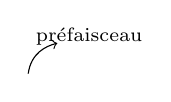
\begin{tikzpicture}[baseline=(p.base),x=1em,y=1em]\node[inner sep=0pt] (p) at (1.8,.7) {\scriptsize\uuline{pré}faisceau};\draw[->] (-.4,-.65) .. controls (-.3,.1) and (.25,.35) .. (.65,.45);\end{tikzpicture}}{\underline{\mathrm{Pr\acute epic}}}_{X'/S'}\deleted{\unsure{X/S}})=\mathrm{Pr\acute epic}(X'/S')\,
\overset{\inserted{=H1(X',\underline O_{X'}^{*})}}{\deleted{={\unsure{H^1}}(X',\underline O_{X'}^{*})=\Gamma(S',\underline H^{1}_{\unsure{X'/S'|X/S}}(\underline O^{*}_{X'}))}} & \deleted{\unsure{X}}\\[.9em]
\underline{\underline{\mathrm{Pr\acute e}\deleted{\unsure{p}}\mathrm{pic}'}}_{X/S}(S')=\Gamma(S',\underset{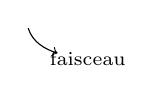
\begin{tikzpicture}[baseline=(p.base),x=1em,y=1em]\node[inner sep=0pt] (p) at (1.8,-.65) {\scriptsize faisceau};\draw[->] (-.35,.45) .. controls (-.2,-.05) and (.25,-.3) .. (.7,-.45);\end{tikzpicture}}{\underline{\mathrm{Pr\acute epic}}'}_{X'/S'})=\mathrm{Pr\acute epic}'(X'/S')\unsure{\deleted{=}|\ne|\deleted{\ne}}\quad=\Gamma(S',\underbrace{\underline H^{1}_{X'/S'}(\underline O^{*}_{X'})}_{\text{faisceau}}) & \\[.7em]
\underline{\underline{\mathrm{Pic}}}_{X/S}(S')=\Gamma(S',\underline{\mathrm{Pic}}_{X'/S'})=\mathrm{Pic}(X'/S')\quad=\widetilde{\underline{\underline{\mathrm{Pr\acute epic}}}}_{X/S}(\deleted{\unsure{X'/S'|X'}}S') & X
\end{array}\)}} 


% Lower portion: relative positions, enclosing lines, circles and hatching follow the sheet.
\figure{\resizebox{\linewidth}{!}{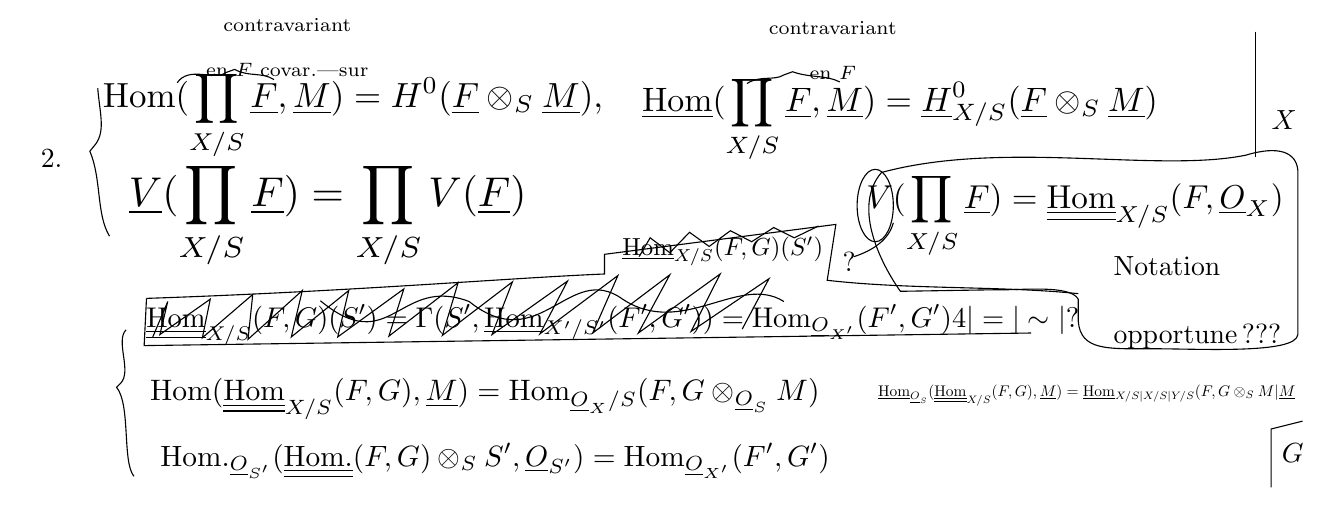
\begin{tikzpicture}[x=.01cm,y=-.01cm,every node/.style={inner sep=0pt,anchor=west}]
\useasboundingbox (0,0) rectangle (1620,590);
\node at (205,22) {\scriptsize\begin{tabular}{c}contravariant\\en $F$ \deleted{\unsure{covar.|sur}}\end{tabular}};
\node at (920,26) {\scriptsize\begin{tabular}{c}contravariant\\en $F$\end{tabular}};
\draw (190,70) .. controls (205,48) and (238,68) .. (252,57) -- (263,53) .. controls (281,63) and (298,56) .. (313,66);
\draw (914,71) .. controls (931,60) and (948,68) .. (961,60) -- (972,56) .. controls (994,64) and (1015,60) .. (1032,69);
\node at (95,112) {\resizebox{6.35cm}{!}{$\displaystyle\mathrm{Hom}(\prod_{X/S}\underline F,\underline M)=H^0(\underline F\otimes_S\underline M),$}};
\node at (780,117) {\resizebox{6.55cm}{!}{$\displaystyle\underline{\mathrm{Hom}}(\prod_{X/S}\underline F,\underline M)=\underline H^0_{X/S}(\underline F\otimes_S\underline M)$}};
\draw (1560,5)--(1560,164);\node at (1580,117) {$X$};
\node at (16,166) {$2.$};
\draw (89,77) .. controls (92,112) and (100,134) .. (83,152) -- (79,157) .. controls (94,192) and (87,237) .. (104,265);
\node at (128,239) {\resizebox{5.05cm}{!}{$\displaystyle\underline V(\prod_{X/S}\underline F)=\prod_{X/S}V(\underline F)$}};
\node at (1065,239) {\resizebox{5.30cm}{!}{$\displaystyle V(\prod_{X/S}\underline F)=\underline{\underline{\mathrm{Hom}}}_{X/S}(F,\underline O_X)$}};
\draw (1077,226) ellipse (23 and 46);
\node at (1035,298) {$?$};
\draw (1050,291) .. controls (1074,283) and (1094,270) .. (1100,248);
\draw (1085,184) .. controls (1240,142) and (1435,185) .. (1548,162) .. controls (1591,149) and (1612,159) .. (1614,181) -- (1614,390) .. controls (1612,415) and (1490,408) .. (1430,408) .. controls (1373,408) and (1338,411) .. (1335,373) -- (1335,345) .. controls (1325,326) and (1260,334) .. (1232,333) -- (1109,335) .. controls (1087,304) and (1046,229) .. (1085,184);
\node at (1358,341) {\begin{tabular}{l}Notation\\opportune\,???\end{tabular}};
\node at (755,284) {\resizebox{2.55cm}{!}{$\deleted{\underline{\mathrm{Hom}}_{X/S}(F,G)(S')}$}};
\node at (150,378) {\resizebox{11.85cm}{!}{$\displaystyle\deleted{\underline{\underline{\mathrm{Hom}}}_{X/S}(F,G)(S')=\Gamma(S',\underline{\mathrm{Hom}}_{X'/S'}(F',G'))=\mathrm{Hom}_{\underline O_{X'}}(F',G')\unsure{4|=|\sim|?}}$}};
% Stepped enclosing stroke and the broad zigzag cancellations of the abandoned definition.
\draw (151,344) .. controls (415,335) and (612,318) .. (733,313) -- (733,288) -- (1027,250) -- (1016,321) .. controls (1120,333) and (1240,328) .. (1335,338);
\draw (151,344)--(148,404)--(1275,388);
\draw (159,393)--(178,348)--(168,390)--(232,345)--(222,394)--(286,339)--(280,396)--(349,334)--(335,393)--(408,334)--(394,393)--(478,332)--(459,392)--(547,324)--(527,391)--(616,323)--(590,390)--(686,322)--(651,389)--(750,315)--(718,388)--(816,314)--(776,388)--(880,313)--(843,386)--(942,319)--(908,383);
\draw (777,291)--(791,267)--(816,286)--(841,260)--(866,278)--(893,258)--(920,272)--(948,254)--(974,267)--(1005,252);
\draw (372,347) .. controls (461,421) and (472,314) .. (561,348) .. controls (651,420) and (688,296) .. (756,345) .. controls (832,395) and (904,312) .. (961,348);
\draw (125,384) .. controls (111,398) and (133,437) .. (118,452) -- (113,457) .. controls (131,479) and (120,552) .. (135,570);
\node at (155,472) {\resizebox{8.50cm}{!}{$\displaystyle\mathrm{Hom}(\underline{\underline{\mathrm{Hom}}}_{X/S}(F,G),\underline M)=\mathrm{Hom}_{\underline O_X\deleted{\unsure{/S}}}(F,G\otimes_{\underline O_S}M)$}};
\node at (1080,467) {\resizebox{5.30cm}{!}{$\displaystyle\underline{\mathrm{Hom}}_{\underline O_S}(\underline{\underline{\mathrm{Hom}}}_{X/S}(F,G),\underline M)=\underline{\mathrm{Hom}}_{\unsure{X/S|\deleted{X/S}|Y/S}}(F,G\otimes_S\unsure{M|\underline M}$}};
\node at (168,550) {\resizebox{8.50cm}{!}{$\displaystyle\mathrm{Hom.}_{\unsure{\underline O_{S'}}}(\underline{\underline{\mathrm{Hom.}}}(F,G)\otimes_S S',\underline O_{S'})=\mathrm{Hom}_{\underline O_{X'}}(F',G')$}};
\draw (1580,584)--(1580,510)--(1620,500);\node at (1593,541) {$G$};
\end{tikzpicture}}}
% Paper watermark, sideways through the table and obscured by the writing.
\margin{\unsure{P.J.A|P.J.} \unsure{VELIN EXTRA}}
% archive sheet number: 8


\clearpage
\scanpage{10}
\hfill\unsure{-} \unsure{Problèmes|Problémes} ouverts
% archive sheet number: 9


\clearpage
\scanpage{11}
\uuline{\unsure{Problêmes|Problèmes}-types à résoudre}

\reversemarginpar
\margin{\tikz[baseline]{\node (a) at (0,0) {\S\,7};\draw (0,0) ellipse (.38 and .59);}}
\fbox{a} A\uline{nneaux de définition} pour des structures sans \unsure{automorphismes|automorphisme}

\margin{\tikz[baseline]{\node at (0,0) {\S\S\,20,21};\draw (0,0) ellipse (.84 and .30);}}
b) Hilbert, Picard sans hypothèse projective
\normalmarginpar\margin{[Résultats partiels]}\reversemarginpar

\margin{\tikz[baseline]{\node at (0,0) {Chap \deleted{\unsure{6|V}}$\underline{\overline{\mathrm{VI}}}$};\draw (0,0) ellipse (.81 and .39);}}
Dual d'un schéma abélien non projectif
\normalmarginpar\margin{\fbox{OK. par Raynaud}}\reversemarginpar

\margin{\tikz[baseline]{\node at (0,0) {\S\S\,3,4};\draw (0,0) ellipse (.75 and .42);}}
\fbox{c} Passage au quotient sans hypothèse de platitude

\noindent\uuline{\hspace{3cm}}

% slanted
\margin{\tikz[baseline,remember picture]{\node[rotate=13] (mumford) at (0,0) {Mumford};\draw[rotate=13] (0,0) ellipse (.81 and .29);}}
\noindent\(\left[\begin{array}{@{}l@{}}
\tikz[baseline,remember picture]{\coordinate (dlabel);}\text{d) }\tikz[baseline,remember picture]{\coordinate (itemd);}\text{Passage au quotient par }\mathrm{Gl}\,\unsure{n|m}\text{, opérant ``sans point fixe''}\\[.5em]
\text{e) Modules de variétés plus ou moins quelconques.}\\
\qquad\tikz[baseline,remember picture]{\coordinate (abel);}\text{Cas des schémas abéliens}
\end{array}\right.\)
\tikz[remember picture,overlay]{\draw[gray,thin](mumford.south) -- (itemd); \draw[gray,thin](mumford.south) to[out=-98,in=178] (abel);}

% slanted
\margin{\tikz[baseline]{\node[align=left,inner sep=1pt] at (0,0) {Mumford -\\Seshadri -\\\unsure{Narashiman|Narasimhan}};\draw (0,0) ellipse (1.01 and .67);}
pour fibrés vectoriels\thinspace; cas fini\thinspace: rédiger}
\noindent\(\left[\begin{array}{@{}l@{}}
\text{f) Classification de fibrés principaux }\inserted{\text{sur }X/Y}\ \text{(par modules)}\\
\quad\text{\unsure{à} groupe affine }\overset{\inserted{G}}{\phantom{G}}\text{ sur }Y\text{, on distingue les cas}\\
\qquad\tikz[baseline,remember picture]{\coordinate (abelg);}\,G\text{ commutatif}\\
\qquad G\text{ non néc commutatif}
\end{array}\right.\)

\margin{\tikz[baseline,remember picture]{\node (seventeen) at (0,0) {\S\,17};\draw[rotate=14] (0,0) ellipse (.53 and .24);}}
\tikz[baseline,remember picture]{\coordinate (itemg);}g) Cas particulier\thinspace; \(G\) fini\thinspace:

\tikz[remember picture,overlay]{\draw[gray,thin] (seventeen.east) to[out=12,in=182] (abelg); \draw[gray,thin] (seventeen.east) to[out=-21,in=168] (itemg);}
% slanted
\margin{Pb mal posé\,?}
h) Cas particulier\thinspace: \(X=P^{1}_{Y},\quad G=\mathrm{Gl}(n)\).

\noindent\uuline{\hspace{3.7cm}}

\margin{Chap $\underline{\overline{\mathrm{VI}}}$\quad\tikz[baseline]{\node at (0,0) {oui};\draw[rotate=13] (0,0) ellipse (.53 and .35);}}
i) Les modules formels d'une variété abélienne \deleted{$A$} sont-ils \uline{simples} sur l'anneau de base\,?

\noindent\uuline{\hspace{3.8cm}}

\fbox{j)} ``Th. du carré'' dans cas non projectif \(-\, -\, -\, -\)

% margin note written sideways
% Paper watermark through the centre.
\margin{\unsure{EXTRA} \unsure{P.J.A|P.J.} \unsure{VELIN}}
% archive sheet number: 10


\cotefile{35}
\scanpage{2}
\noindent\hfill\margin{\handwritten{zurück an G.}}\par

\noindent SGA 7\qquad Groupe de Monodromie en Géométrie Algébrique

\reversemarginpar
\noindent\margin{\handwritten{Gr}}I\quad G\deleted{\unsure{ad|ed}}énéralités sur le g\deleted{o}roupe de monodromie locale. Le théorème de monodromie par voie arithmétique.

\noindent\margin{\handwritten{Gr}}II\quad Cas d'action\deleted{s} résoluble\deleted{s} d'ungroupe fondamental (variante du \deleted{groupe} théorème de monodromie).

\noindent\margin{\handwritten{Gr}}III\quad Le théorème de monodromie par voie géométrique.\normalmarginpar
\margin{\handwritten{\figure{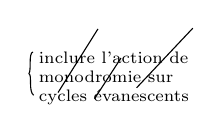
\begin{tikzpicture}[x=1cm,y=1cm,scale=.86,transform shape]
\node[anchor=north west,align=left,inner sep=0pt,font=\scriptsize] at (.14,.06)
{\deleted{inclure l'action de}\\
 \deleted{monodromie sur}\\
 \deleted{cycles évanescents}};
\draw (.06,.05) .. controls (-.01,.03) and (.04,-.22) .. (0,-.27)
 .. controls (.05,-.29) and (-.01,-.53) .. (.07,-.59);
\draw (.43,-.55)--(1.02,.39) (.97,-.64)--(1.36,-.04) (1.59,-.48)--(2.42,.40);
\end{tikzpicture}}}}

\reversemarginpar
\noindent\margin{\handwritten{Gr}}IV\quad Propriétés générales des groupes de cycles évanescents. Cas des points singul\deleted{\unsure{ei|ee}}iers isolés de la fibre spéciale.

% slanted
\noindent\margin{\handwritten{Gr\par
\figure{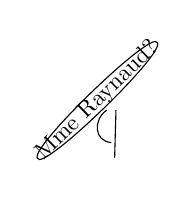
\begin{tikzpicture}[scale=.84,transform shape]
\begin{scope}[rotate=44,transform shape]
\node[inner sep=1.1pt] (q) {Mme Raynaud?};
\draw (q.west) .. controls (q.north west) and ([xshift=3pt]q.north east) .. (q.east)
 .. controls (q.south east) and ([xshift=-3pt]q.south west) .. (q.west);
\end{scope}
\draw (q.south) .. controls +(-.21,-.15) and +(-.26,.02) .. ++(.07,-.49);
\draw ([xshift=4pt]q.south) -- ++(-.02,-.72);
\end{tikzpicture}}}}V\quad Groupe de monodromie opérant sur le groupe fondamental: théorèmes d'action modérée et d'action essentiellement modérée.

\noindent\margin{\handwritten{Mme Raynaud\par\deleted{Mme Raynaud}}}\deleted{VI}\handwritten{\inserted{\unsure{App.|Arr.}}}\quad Application: présentation finie des groupes fondamentaux géométrique\unsure{s}

\noindent\margin{\handwritten{\uline{Rim}}}\handwritten{\inserted{$\underline{\overline{\mathrm{VI}}}$\quad Modules formels (ist bei Deligne)}}

\noindent\margin{\handwritten{Gr}}VII\quad Biextensions de faisceaux de groupes.

\noindent\margin{\handwritten{Gr}}\handwritten{\inserted{$\underline{\overline{\mathrm{VIII}}}$\quad Extensions et biextensions de schémas en groupes \unsure{pr|par} $G_m$}}

% The outlined typescript above this line has a downward point between the two words.
\noindent\margin{\handwritten{Gr}}\deleted{\unsure{VIII}}\handwritten{$\underline{\overline{\mathrm{IX}}}$}\quad Application\handwritten{s} au modèle de Néron: \deleted{le} théorème \tikz[baseline,remember picture]{\coordinate (orthogpoint);}
\tikz[overlay,remember picture]{
\node[anchor=south west,inner sep=2pt] (orthogtext) at ([xshift=-1.55cm,yshift=.38cm]orthogpoint) {\inserted{d'orthogonalité, théorème}};
\draw (orthogtext.north west) .. controls ([xshift=-.28cm]orthogtext.north west) and ([xshift=-.28cm]orthogtext.south west) .. (orthogtext.south west)
 -- ([xshift=-.13cm,yshift=.33cm]orthogpoint) -- ([yshift=-.13cm]orthogpoint)
 .. controls ([yshift=.22cm]orthogpoint) and ([xshift=.10cm,yshift=.32cm]orthogpoint) .. ([xshift=.25cm,yshift=.33cm]orthogpoint)
 -- (orthogtext.south east) .. controls ([xshift=.25cm]orthogtext.south east) and ([xshift=.25cm]orthogtext.north east) .. (orthogtext.north east);
} de réduction semi-stable.\handwritten{\tikz[baseline]{\draw[line cap=round] (.01,.045)--(.045,.020) (.11,.035)--(.155,.025) (.23,.059)--(.28,.046);}}

\noindent\margin{\handwritten{\deleted{Deligne}}}
\figure{\resizebox{\linewidth}{!}{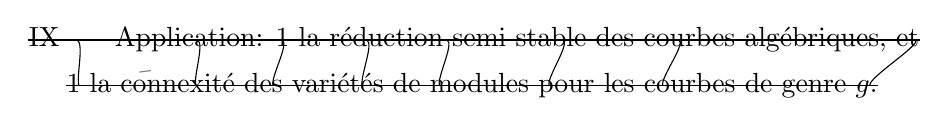
\begin{tikzpicture}
\node[anchor=west,inner sep=0pt] (a) at (0,0) {\deleted{IX}\qquad \deleted{Application: {\deleted{\illegible{1} la}} réduction semi-stable des courbes algébriques, {\deleted{et}}}};
\node[anchor=west,inner sep=0pt] (b) at (.48,-.58) {\deleted{{\deleted{\illegible{1} la}} \tikz[overlay]{\draw[gray] (.24,.26)--(.39,.28);}connexité des variétés de modules pour les courbes de genre $g$.}};
\draw (a.west) -- (a.east);
\draw (b.west) -- (b.east);
\foreach \p/\q in {.055/.016,.19/.16,.285/.255,.38/.365,.47/.46,.60/.595,.73/.735,.995/.99}
{\path (a.west) -- (a.east) coordinate[pos=\p] (t);
 \path (b.west) -- (b.east) coordinate[pos=\q] (u);
 \draw (t) .. controls +(0.09,-.05) and +(-.04,.09) .. (u);}
\end{tikzpicture}}}

% archive sheet number: 1


\par\clearpage
\normalmarginpar
\scanpage{3}
\noindent\hfill\margin{\unsure{zurück} an ·\tikz[baseline=(g.base)]{\node[inner sep=0pt] (g) {G};\draw ([xshift=-1pt,yshift=-4pt]g.south west)--([xshift=4pt,yshift=1pt]g.south east);}}\par

\noindent SGA 7

\noindent D\quad $\underline{\overline{\mathrm{X}}}$\quad Intersections \tikz[baseline]{\draw[line cap=round] (0,.035)--(.065,.04) (.12,.04)--(.151,.043) (.211,.034)--(.295,.057);}

\noindent D\quad $\underline{\overline{\mathrm{XI}}}$\quad Int. complètes

\noindent D\quad $\underline{\overline{\mathrm{XII}}}$\quad \unsure{Quadriques|Quadrique}

\noindent D\quad $\underline{\overline{\mathrm{XIII}}}$\quad Points quadr. ordinaires. Pic-\unsure{Lef|lef} faible

\noindent D\quad $\underline{\overline{\mathrm{XIV}}}$\quad Formule Milnor

\diagram{\(\begin{array}{@{}ll@{}}
\text{D}&\underline{\overline{\mathrm{XV}}}\\
\text{D}&\underline{\overline{\mathrm{XVI}}}
\end{array}
\left\{\begin{array}{l}
\text{Picard'-Lefschetz}\\
\text{Picard-Lefschetz}
\end{array}\right.
\;\tikz[baseline]{\draw[gray,thin] (0,.86) .. controls (.035,.62) and (-.045,.06) .. (.013,-.23);}
\)}

\noindent K\quad
$\begin{array}{@{}c@{}}
\underline{\overline{\mathrm{XVII}}}\\[-2pt]
\underline{\overline{\mathrm{XVIII}}}
\end{array}\,\Bigg|$\quad
Pinceaux de Lefschetz~: \uline{existen}ce \tikz[baseline]{\draw[gray,thin] (.18,.62) .. controls (.19,.36) and (.08,.18) .. (.07,-.09) -- (.11,-.17);\draw[gray,thin] (.20,.58) .. controls (.15,.25) and (.01,-.02) .. (-.01,-.20) -- (-.035,-.16);\draw[line cap=round] (-.06,0)--(.17,.34) (-.04,-.015)--(.18,.31) (.03,.013)--(.25,.35);} \uuline{\unsure{étude|études} \unsure{cohomologique|cohomologiques}}

\diagram{D\quad $\underline{\overline{\deleted{\unsure{\mathrm{XVIII}}}\mathrm{XIX}}}$\quad
\uuline{Th de Noether}
$\left\{\begin{array}{l}
\text{via Hodge-Deligne}\\
\text{via \uuline{\underline{\text{Katz}}}}
\end{array}\right.$}

\diagram{\begin{tabular}{@{}c@{\ }p{.84\linewidth}@{}}
$\mathrm{K}\left\{\rule{0pt}{12ex}\right.$ &
\begin{minipage}[c]{\linewidth}
\noindent $\deleted{\underline{\overline{\unsure{\mathrm{XIX}|\mathrm{XX}}}}}\;
\underline{\overline{\mathrm{XX}}}\deleted{\unsure{\mathrm{I}}}$\quad Th. de Griffiths.

\noindent $\underline{\overline{\mathrm{XXI}}}$\quad \deleted{\unsure{Théorème|Théor}} Niveau de la coh. des intersections \unsure{complètes|completes}

\noindent $\underline{\overline{\mathrm{XXII}}}$\quad \deleted{\unsure{Form.|Fon.}} Calcul de la \unsure{fonction} $\deleted{\unsure{z}}\zeta$ mod $p$.
\end{minipage}
\end{tabular}}

\figure{\begin{tikzpicture}\draw (0,0) .. controls (.29\linewidth,.45) and (.76\linewidth,.57) .. (.98\linewidth,.46);\end{tikzpicture}}

\noindent Exposés transcendants (Lê Dũng Tráng ?)

\[
\underline{\mathbb{F}_{q}\qquad \#\qquad \mathrm{card}}\quad\unsure{.}
\]

% archive sheet number: 2


\par\clearpage
\normalmarginpar
\scanpage{4}
\noindent\margin{\vspace*{5.3\baselineskip}SGA 7}\par

% The two long pen strokes, including their returns at the bottom, cross several rows.
\begingroup
\small
\setlength{\arraycolsep}{3pt}
\renewcommand{\arraystretch}{2.05}
\diagram{\figure{\resizebox{\linewidth}{!}{%
\begin{tikzpicture}
\node[anchor=south west,inner sep=0pt] (refs) at (0,0) {%
$\begin{array}{@{}lll@{}}
\text{[17]}&\text{Griffiths, P.}&\text{\raisebox{.6ex}{\unsure{-|\textquoteleft}}Yale talk}\\
\text{[18]}&\text{Grothendeik, A.}&\text{\unsure{Inventiones|Inventionis}}\\
\text{[19]}&\text{\rlap{\hspace*{-.9em}\raisebox{1.05em}{\inserted{Deligne-}}}\tikz[baseline,overlay]{\draw (-.15,-.10) .. controls (-.15,.25) and (.66,.14) .. (.76,.42);}Grothendeik, A.}&\text{S.G.A. on monodromy}\\
\text{[20]}&\text{Lendman, A.}&\text{Berkeley thesis (196\deleted{\unsure{4|0}}6)}\\
\text{[21]}&\text{Lieberman, D.}&\text{Higher Picard varieties}\\
\text{[22]}&\text{Schmid, W.}&\text{On a Conjecture of Langlands}\\
\text{[23]}&\text{Wu, H.}&\text{Acta paper\textquoteright}
\end{array}$};
\begin{scope}[x={(refs.south east)},y={(refs.north west)}]
\draw[gray] (.305,.90) .. controls (.23,.78) and (.06,.16) .. (.041,-.14)
    .. controls (.030,-.20) and (.062,-.14) .. (.101,-.076);
\draw (.784,1.11) .. controls (.68,.82) and (.49,.13) .. (.426,-.025)
    .. controls (.414,-.052) and (.405,-.051) .. (.400,-.040);
\end{scope}
\end{tikzpicture}}}}
\endgroup

% archive sheet number: 3


\par\clearpage
\normalmarginpar
\scanpage{5}
\mspage{\handwritten{\tikz[baseline=(f.base)]{\node[inner sep=1pt] (f) {11bis};\draw (f.north west) .. controls ([yshift=-5pt]f.south west) and ([yshift=-5pt]f.south) .. ([yshift=-5pt]f.south east);}}}
\noindent\handwritten{\tikz[overlay]{\draw (-1.3,.30)--(-1.24,.41);\draw (-1.14,.41)--(-.99,.29);}}
\handwritten{\tikz[overlay]{\draw (.72\linewidth,.35) .. controls (.73\linewidth,.23) and (.732\linewidth,.23) .. (.733\linewidth,.35);}}
% The three large cancellation strokes cross the two numbered sections.
\figure{\begin{tikzpicture}
\node[anchor=north west,inner sep=0pt] (body) at (0,0) {\begin{minipage}{.93\linewidth}
\small
\noindent
\deleted{1.3.{\deleted{\unsure{2|3}}}{\unsure{3|2}}.}\quad
\deleted{\inserted{La terminologie de 1.3.1 {\deleted{et 1.3.2}} s'étend aussitôt au cas où}}
\deleted{\deleted{Revenons au cas {\unsure{où|ou}} on se donne deux Groupes $P$ et $Q$ sur $G$}}
\deleted{on a un {\uline{bitorseur}} {\deleted{\unsure{osus|sous}}} {\inserted{$E$}} sous{\deleted{$(G$}} $(G_{P},G_{P})$, {\deleted{resp{\unsure{.|,}} sous $({G\unsure{,}}_{P\mathrm{x}Q},G_{P\mathrm{x}Q})$,}} étant entendu qu'une rigidification du bitorseur $E$ doit être un isomorphisme de $e_{P}(E)$ avec le b{\deleted{o}}it{\deleted{r}}o{\deleted{o}}rs{\deleted{\unsure{e|u}}}eur trivial $\,{}_{s}G_{d}$, {\deleted{donc}} {\inserted{i.e.}}{\handwritten{\tikz[baseline]{\draw (0,-.04) .. controls (.035,.14) and (.16,.06) .. (.19,.25);}}} est défini par une section $e_{E}$ de $e_{P}(E)$ qui est {\uline{centrale}}, i.e. qui satisfait à la condition $g.e_{E}=e_{E}.g\quad(g\mathrel{\handwritten{\unsure{\in|\epsilon}}}G(S)$ . On étend de même la terminologie des birigidifications au cas des bitorseurs.}

\noindent\deleted{1.3.4.}\quad
\deleted{Revenons au cas où on se donne deux Groupes $P$ et {\deleted{$Q$}} {\handwritten{\inserted{$G$}}}, et choisissons la section unité $e_{P}$ pour définir des rigidifications de bitorseurs sur $P$, et des birigidifications de bitorseurs sur $P\mathrm{x}P$. On a des foncteurs naturels}

\begingroup
\csname tagsleft@true\endcsname
\diagram{\[
\begin{tikzcd}[ampersand replacement=\&,column sep=1.7em]
\deleted{\underline{\mathrm{Ext}}(P;\unsure{G'|G})} \arrow[r,"{\handwritten{i}}"]
\& \deleted{\underline{\mathrm{Bitorsrig}}(P,G)} \arrow[r,"{\handwritten{\rlap{\raisebox{.35ex}{\hspace{-.12em}\(\color{gray!55}\scriptstyle\delta\)}}\delta}}"]
\& \deleted{\underline{\mathrm{Bitorsbirig}}(P,P;G){,}}
\end{tikzcd}
\tag*{\deleted{(1.3.4.1)}}
\]}
\endgroup

\noindent\deleted{où les trois expressions écrites désignent respectivement la catégorie des extensions de {\handwritten{\tikz[baseline,overlay]{\node[anchor=south west,inner sep=0pt] at (-.15,.31) {\inserted{Groupes de}};\draw (-.08,-.12) .. controls (-.08,.24) and (.06,.26) .. (.35,.26) .. controls (.75,.26) and (1.15,.24) .. (1.35,.32) .. controls (1.40,.35) and (1.40,.43) .. (1.32,.42);}}}$P$ par $G$, la catégorie des {\deleted{b}}{\handwritten{B}}itorseurs sous $(G_{P},G_{P})$ rigidifiés pour{\textasciigrave} $e_{P}$, et la catégorie des {\deleted{t}}b{\deleted{o}}it{\deleted{r}}orseurs sous$(G_{P\mathrm{x}P},G_{P\mathrm{x}P})$ birigidifiés pour $(e_{P},e_{P})$. On {\deleted{prend}} définit le foncteur $i$ en associant à l'extension $E$ de $P$ par $G$ le {\deleted{torseu}} bitorseur correspondant sur $P$ (1.1.6), rigidifié par la sectio{ń} unité de $E$. O{\deleted{\unsure{n}}}{\handwritten{n}} {\unsure{definit|définit}} le foncteur $\handwritten{\delta}$ par la formu{\deleted{o}}le}
\end{minipage}};
\begin{scope}[x={(body.north east)},y={(body.south west)}]
\draw (.44,.11) .. controls (.35,.27) and (.00,.66) .. (-.047,.725)
 .. controls (-.053,.736) and (-.054,.746) .. (-.043,.75);
\draw (.82,.078) .. controls (.73,.30) and (.50,.69) .. (.31,1.035);
\draw (.91,.505) .. controls (.915,.62) and (.78,.86) .. (.655,1.03);
\end{scope}
\end{tikzpicture}}
% archive sheet number: 4


\cotefile{48}
\scanpage{2}
\noindent\hfill Plan EGA $\overline{\text{\uline{VI}I}}$

% archive sheet number: 1
\clearpage


\scanpage{3}
\noindent EGA \uline{Chap\unsure{.}\ $\overline{\mathrm{VI}}$}\qquad
\uline{\unsure{Schèmas|Schémas} en gpes et \rlap{\raisebox{1.1em}{\inserted{\unsure{torseurs|Torseurs}}}}\deleted{fibrés \unsure{principaux} \unsure{homogènes}}}

\noindent\textcircled{A}\quad \uline{Propriétés générales}

\noindent\uline{\S~1}\quad Histoires \unsure{des|de|du} passage d'un pt à \unsure{tout|tous}, de propriétés ouvertes / propriétés générales des morphismes

\noindent\uline{\S~2}\quad Composantes neutre. Dimensions. Séparation

\noindent\uline{\S~3}\quad Groupes affines

% slanted
\reversemarginpar
\noindent\llap{\tikz[baseline]{\node[rotate=25,anchor=east,inner sep=1pt] at (-.2,0) {\shortstack[r]{sur\\un corps}};\draw (0,.9) .. controls (-.18,.7) and (.08,.14) .. (-.24,.1) .. controls (.08,.04) and (-.02,-.7) .. (.15,-.9);\draw[gray] (.04,.82) .. controls (-.02,.5) and (.1,.14) .. (-.19,.07);}\hspace{.4em}}\uline{\S~4}\quad Sous-gpes engendrés
\normalmarginpar

\noindent\uline{\S~5}\quad Passage au quotient: \inserted{\deleted{(sur un corps)}}espaces hom. et gpes quotients.

\noindent\uline{\S~6}\quad $G^{\unsure{\tau|t}}$ si $\unsure{G|C}$ comm (cf \unsure{FDTE|TDTE} $\overline{\text{\uline{VI}}}$ n\textsuperscript{\uline{o}}~1)

\noindent\textcircled{\deleted{B}B}).\quad \uline{Études infinitésimales}

\noindent\S~7\quad Questions d'extensions infinitésimales. (cf SGAD $\overline{\text{\uline{II}}}$)

\noindent\S~8\,: \quad Hyperalgèbre d'un gpe alg. et op. diff inv

\noindent\S~9.\quad Frobeniusiennes

\noindent``\S~10''\quad \deleted{\unsure{Algè|Alg}} Groupes radiciels et $p$-algèbres de Lie

\noindent\inserted{\S~11\quad Dualité de Cartier.}

\noindent\deleted{\textcircled{C}\quad \S.\quad \uline{Dualité de Cartier}}

\noindent\textcircled{C}\quad \uline{Groupes de t. \unsure{m.}}\ ; \uline{propriétés de rigidité liées aux p\textsuperscript{ts} d'ordre \unsure{fini}.}

\noindent\S~12.\quad Maximum : SGAD $\overline{\text{\uline{VIII}}}$, $\overline{\text{\uline{IX}}}$, $\overline{\text{\uline{X}}}$

% archive sheet number: 2
\clearpage


\scanpage{4}
\mspage{\handwritten{(30}}
\begingroup
\reversemarginpar
\makeatletter\tagsleft@true\makeatother
\noindent\margin{\handwritten{$\varphi\qquad \varepsilon_{\xi'}$}}%
\handwritten{\tikz[baseline=-.2ex]{\draw (0,0) .. controls (.13,.16) and (.36,.24) .. (.43,.21) .. controls (.45,.19) and (.45,.17) .. (.45,.16);}}\,
Lorsque $\handwritten{\varphi}$ est de la forme $\handwritten{\varepsilon_{\xi'\raisebox{.45ex}{$\scriptstyle\deleted{\unsure{\xi'|\xi}}$}}}$, donc
\margin{\handwritten{$\varphi$}}
\[
\handwritten{\varphi} \handwritten{\simeq} \mathop{\underset{\handwritten{\longrightarrow}}{\mathrm{lim}}}\limits_j {X'_j}^{\handwritten{\unsure{\vee|v}}}\ , 
\]
on a donc une bijection naturelle
\margin{\handwritten{$\varepsilon_{\xi}\quad\varepsilon_{\xi'}\qquad .$}}
\[
\operatorname{Hom}\bigl(\handwritten{\varepsilon_{\substack{\deleted{\unsure{\xi}}\\[-.4ex]\xi}}},\handwritten{\varepsilon_{\substack{\deleted{\unsure{\xi}}\\[-.4ex]\xi\unsure{'}}}} ,\bigr)
 \handwritten{\simeq} \mathop{\underset{\handwritten{\longleftarrow}}{\mathrm{lim}}}\limits_i \mathop{\underset{\handwritten{\longrightarrow}}{\mathrm{lim}}}\limits_j \operatorname{Hom}_{X}(X'_j,X_i)\handwritten{\deleted{\unsure{,|.}}}\qquad .
\tag*{$(*)$}
\]

\noindent D'autre part on a (dans la catégorie des préschémas)
\margin{\handwritten{$\deleted{\unsure{\xi}}$}}
\[
\bar X(\handwritten{\xi}) == \mathop{\underset{\handwritten{\longleftarrow}}{\mathrm{lim}}}\limits_i X_i\handwritten{\deleted{\xi}}\ ,\quad
\bar X(\handwritten{\xi}') = \mathop{\underset{\handwritten{\longleftarrow}}{\mathrm{lim}}}\limits_j X'_j\ ,
\]
d'où
\[
\handwritten{\tikz[baseline=-.2ex]{\draw (0,0) .. controls (.08,-.03) and (.18,.03) .. (.23,.08);}}\; \operatorname{Hom}_{X}(\bar X(\handwritten{\xi}'),\bar X(\handwritten{\xi})) \handwritten{\simeq}
 \mathop{\underset{\handwritten{\longleftarrow}}{\mathrm{lim}}}\limits_i \operatorname{Hom}_{X}(\bar X(\handwritten{\xi}'),X_i)\ ,
\]
\margin{\handwritten{\tikz{\draw (0,0) .. controls (.04,.18) and (.27,.10) .. (.49,.28) .. controls (.58,.35) and (.56,.45) .. (.54,.47);}}}
d'autre part, comme $X_i$ est loc\inserted{\handwritten{\tikz[baseline=(w.base)]{%
\node[anchor=base west,rotate=14,inner sep=.3pt] (w) at (0,0) {alement};
\draw (-.04,-.17) .. controls (-.01,.08) and (.42,.04) .. (.85,.27) .. controls (.98,.34) and (1.04,.41) .. (.99,.42);
}}} de présentation finie sur $X$\handwritten{, on a}
\[
\operatorname{Hom}_{\handwritten{X}}(\bar X(\handwritten{\xi}'),X_i) \handwritten{\simeq}
 \mathop{\underset{\handwritten{\longrightarrow}}{\mathrm{lim}}}\limits_j \operatorname{Hom}_{X}(X_j,X_i)\handwritten{,}
\]
d'où
\[
\operatorname{Hom}_{X}(\bar X(\handwritten{\xi}'),\bar X(\handwritten{\xi})) \handwritten{\simeq}
 \mathop{\underset{\handwritten{\longleftarrow}}{\mathrm{lim}}}\limits_i \mathop{\underset{\handwritten{\longrightarrow}}{\mathrm{lim}}}\limits_j \operatorname{Hom}_{X}(X'_j,X_i)\ .
\tag*{$(**)$}
\]

\noindent La comparaison de $(*)$ est $(**)$ donne la\handwritten{$\mid$}conclusion voulue (moyennant une verification de compatibilités, laissé\deleted{\unsure{n|e|s}}e au lecteur).

% slanted
\noindent\margin{\handwritten{\begin{tikzpicture}[baseline,scale=.84]
\node[rotate=13,inner sep=1pt] (m) at (0,0) {\scriptsize\unsure{pas} d'espacement};
\draw[rotate=13] (0,0) ellipse [x radius=1.08cm,y radius=.31cm];
\draw (.96,.13) .. controls (1.13,.06) and (1.29,.04) .. (1.42,.05);
\draw (1.53,.33) .. controls (1.39,.27) and (1.34,-.18) .. (1.60,-.21);
\end{tikzpicture}}}%
b) \uline{Le foncteur envisagé est essentiellement surjectif:}

\noindent 7.9.1.\quad Remarquons d'abord que si $C$ est un site où les $\mathop{\underset{\handwritten{\longleftarrow}}{\mathrm{lim}}}\limits$ finies sont représentable, $\handwritten{\widetilde}{C} = \underline{E}$ le topos correspondant alors\handwritten{,} tou\deleted{s}\handwritten{t}%
\margin{\handwritten{,\quad t}}
foncteur\deleted{s} fibre\deleted{s} $\handwritten{\overset{\deleted{\unsure{\varphi|\xi}}}{\varphi}}$ sur $\underline E$ peut se représenter comme une ``limite''
\margin{\handwritten{$/\quad /\quad\varphi$}}
inductive pseudo-filtrante connex\deleted{\unsure{e}}\handwritten{e}\handwritten{''} d\deleted{e}\handwritten{e} foncteurs de la forme
\margin{\handwritten{e\quad e}}
\margin{\handwritten{$]\,[ $}}
\[
\handwritten{\check}{Y}(F) == F(Y) = \operatorname{Hom}(\handwritten{\widetilde}{Y},F),\handwritten{\big]\big[}\, Y\handwritten{\in}\operatorname{Ob} C\handwritten{,}
\]
(ou $\handwritten{\widetilde}{Y}$ est le faisceau associé à $Y$)\handwritten{,} de la façon suivante. On considèr\deleted{\unsure{e|s}}\handwritten{e}
\margin{\handwritten{,}}
la catégorie\handwritten{$\mid C_{\substack{\deleted{\unsure{\xi|\varphi}}\\[-.4ex]\varphi}}$} des couples $(Y,\handwritten{\xi})$, avec $Y\handwritten{\in}\operatorname{Ob} C$, $\handwritten{\xi}\handwritten{\in\varphi}(\handwritten{\widetilde}{Y})$
\margin{\handwritten{$C_{\varphi}$}}
\endgroup

% archive sheet number: 3
\clearpage


\scanpage{5}
\noindent\tikz[baseline=(n.base)]{\node[inner sep=0pt] (n) {D};\draw (n.center) ellipse (.82em and .88em);\draw (n.center) ellipse (1.08em and 1.13em);\draw ([xshift=-1em,yshift=-.35em]n.center) .. controls ([xshift=-1.04em,yshift=.75em]n.center) and ([xshift=-.30em,yshift=1em]n.center) .. ([xshift=.35em,yshift=.96em]n.center);}\quad
\uline{Propriétés générales des} \uline{schémas \unsure{abéliens|abeliens}} \uline{et \unsure{parabeliens|parabéliens}}

\figure{\makebox[\linewidth][l]{\hspace*{3em}\tikz{\foreach \y in {0,.12,.24,.36,.48}{\fill (0,\y) ellipse (.012 and .020);}}}}

\noindent\tikz[baseline=(n.base)]{\node[inner sep=0pt] (n) {E};\draw (n.center) ellipse (.68em and .96em);\draw (n.center) ellipse (.88em and 1.12em);}\quad
\uline{Extensions des schémas \unsure{abéliens|abeliens} par gpes affines}

\noindent\hspace*{7em} (th. de Chevalley....).

\figure{\makebox[\linewidth][l]{\hspace*{3em}\tikz{\foreach \y/\l in {0/.08,.13/.04,.26/.06,.39/.06,.52/.09}{\draw (0,\y) -- ++(0,\l);}}}}

\noindent%
\figure{\begin{tikzpicture}[baseline=(t.base)]
\node[anchor=base,font=\scriptsize] (letter) at (-1.40,0) {\deleted{\unsure{F|D}}D};
\draw (letter.center) ellipse (2.06em and .91em);
\draw (letter.center) ellipse (2.37em and 1.15em);
\node[anchor=south west,inner xsep=2pt] (ins) at (.65,.50) {\inserted{Groupes classiques et}};
\draw (ins.south west) .. controls +(.12,.14) and +(-.19,0) .. (ins.north west)
  .. controls +(.30,.09) and +(-.20,.07) .. (ins.north east)
  .. controls +(.23,0) and +(.37,.08) .. (ins.south east) -- (ins.south west);
\draw (ins.south west) -- (.19,.50) .. controls (-.16,.50) and (-.22,-.07) .. (-.10,-.17);
\node[anchor=base west,inner sep=0pt] (t) at (0,0) {\uline{torseurs} \uline{sous gpes classiques}};
\end{tikzpicture}}\margin{(N'importe où)}

\noindent\hfill et théorème de l'isotrivialité sur un corps \unsure{(P.)|(?)}.

\noindent\tikz[baseline=(n.base)]{\node[inner sep=0pt] (n) {\scriptsize\deleted{\unsure{E|F}}\unsure{F|E}};\draw (n.center) ellipse (2.20em and .95em);\draw (n.center) ellipse (2.40em and 1.18em);}\quad
Modèles de Néron (?)

\noindent\hfill Un paragraphe de variations sur le ``th. \unsure{du|des} carré''?

\noindent \unsure{Ref|Réf}\quad \begin{tabular}[t]{@{}l@{}}
SGAD\\
BIBLE\\
``Boulder''\\
Livre(s) Mumford
\end{tabular}

% archive sheet number: 4
\clearpage


\scanpage{6}
\mspage{\handwritten{(29}}
\begingroup
\makeatletter\tagsleft@true\makeatother
\[
\underline{\mathrm{Pt}}(X)^{\unsure{\circ|o|0}}\dashrightarrow
\underline{\mathrm{Pt}}(\handwritten{\widetilde}{X_{\text{ét}}})\ ,
\tag*{$(*)$}
\]
où le premier membre est défini dans 7.6.. Ceci posé, on a le

\noindent\uline{Théorème} 7.9.\quad Soit $X$ un préschéma. Le foncteur précédent $(*)$ est une \uline{an\deleted{\unsure{it|ti}}\handwritten{ti}-équivalence} de la catégorie des points géomètriques sur $X$ (avec comme morphismes les flèches des spécialisation) avec la catégorie des foncteurs fibres sur le topos étale $\handwritten{\widetilde}{X_{\text{ét}}}$.

Comme ce théorème ne servira plus dans la suite du séminaire nous nous bornons ici à une esquisse de démonstration, où nous nous permettrons certaines libertés avec les questions d'Univers.

a) \uline{Le foncteur envisagé est pleinement fidèle}. Pour tout $X\handwritten{\in}\operatorname{Ob} X_{\text{ét}}$, soit $X^{\handwritten{\unsure{\vee|v}}}: \handwritten{\widetilde}{X_{\text{ét}}} \dashrightarrow (\mathrm{Ens})$ défini par
\[
\handwritten{\check}{X}(F) = \operatorname{Hom}(X,F) = F(X).
\]

\noindent Notons que le foncteur fibre
\[
\handwritten{\varepsilon_{\xi}} : F \handwritten{\rightsquigarrow} F_{\handwritten{\xi}}
\]
peut s'écrire
\[
\handwritten{\varepsilon_{\xi}} \handwritten{\simeq} \mathop{\underset{\handwritten{\longrightarrow}}{\mathrm{lim}}}\limits_i X_i^{\handwritten{\vee}}\ ,
\]
où les $X_i$ sont des préschémas affines étales sur $X$ indexées par une certeine catégorie pseudo-filtrante (cf 4.3. et 4.5.). On a donc pour tout foncteur $\handwritten{\varphi}: \handwritten{\widetilde}{X_{\text{ét}}} \dashrightarrow (\mathrm{Ens})$:\margin{\tikz{\fill (0,0) circle (.018);\fill (.08,.12) circle (.018);}}
\[
\operatorname{Hom}(\handwritten{\varepsilon_{\xi}},\handwritten{\varphi}) \mathrel{\mathop{\text{-\kern.04em-}}\limits^{\handwritten{\sim}}} \mathop{\underset{\handwritten{\longleftarrow}}{\mathrm{lim}}}\limits_{\handwritten{i}} \operatorname{Hom}(X_i^{\handwritten{\vee}},\handwritten{\varphi})\ ,
\]
d'autre part il est bien connu que l'on a un isomorphisme bifonctoriel
\[
\operatorname{Hom}(X_i^{\handwritten{\vee}},\handwritten{\varphi}) \mathrel{\mathop{\text{-\kern.04em-}}\limits^{\handwritten{\sim}}} \handwritten{\varphi}(X_i)\ .
\]

\figure{\begin{tikzpicture}[x=1cm,y=1cm]
\draw (0,0) .. controls (.45,-.76) and (1.34,-1.79) .. (1.83,-2.47);
\end{tikzpicture}}
\endgroup

% archive sheet number: 5


\cotefile{66}
\scanpage{2}
\noindent\begin{minipage}[t]{.10\linewidth}
\figure{\begin{tikzpicture}[x=.28cm,y=.28cm]
\draw[gray!45,very thin] (.14,3.5) .. controls (.09,2.5) and (.12,.85) .. (.25,.25);
\draw (.14,1.87) -- (1.33,3.58);
\draw[gray!45,very thin] (1.46,3.58) -- (.57,.52) .. controls (.46,.1) and (.71,-.06) .. (.92,0);
\draw (.80,1.37) .. controls (1.34,2.02) and (1.81,2.78) .. (2.14,3.14);
\end{tikzpicture}}
\end{minipage}\hspace{.02\linewidth}%
\begin{minipage}[t]{.86\linewidth}
\tikz[baseline=(yr.base)]{\node[inner sep=2pt] (yr) {1964}; \draw (yr.north west) -- (yr.south west) -- (yr.south east) -- (yr.north east);}
\hfill Numéros cerclés sont sans doute difficiles.

\uline{Travaux de thèses}

\deleted{[\unsure{Collection} 1964]}
\end{minipage}%
\begingroup\setlength{\marginparwidth}{2.9cm}\margin{(N.B. Les sujets 1 à 10 et 20, 21, \tikz[baseline=-.5ex]{\node[anchor=south,inner sep=1pt] (nbins) at (0,.08) {\inserted{26, 27, 28}};\draw (-.85,.05)--(-.85,-.12)--(.85,-.12)--(.85,.05);} sont de nature essentiellement cohomologique \unsure{$\zeta$|$\xi$|§|$g$}. 10, 19, 23, 24, 25 \unsure{relèvent|relévent} de la théorie des intersections ; 11, 12, 13 se rattachent à la th. de Néron. 14, 15, 22 th. du topos...; 17, 18 yoga de représentabilité, de foncteurs)}\endgroup

1) Topologie et cohomologies $\mathrm{fppf}$ : formalisme général
\inserted{\textcircled{\scriptsize $*$} \tikz[baseline=(cr.base)]{\node[inner sep=2pt] (cr) {[Rela\uline{tion avec coh-mologie cristall}ine]};\draw[gray!55,thin] (cr.west) .. controls ([yshift=5pt]cr.north west) and ([yshift=4pt]cr.north east) .. (cr.east) .. controls ([yshift=-3pt]cr.south east) and ([yshift=-2pt]cr.south west) .. (cr.west);}}

\reversemarginpar
\textcircled{2}\margin{[subordonné à 1), 11)]} \rule[.45ex]{3.9em}{.45pt} : dualité (\tikz[baseline=(loc.base)]{\node[inner sep=0pt] (loc) {locale};\draw[gray!60] (-.48,-.14) .. controls (-.32,-.24) and (-.17,-.08) .. (0,-.16) .. controls (.16,-.24) and (.31,-.1) .. (.48,-.16);}, globale).

\textcircled{3}\margin{[subordonné à 2), donc à 1) et 11)]} Partie $p$-primaire dans formule de Ogg-Chafarévitch

\normalmarginpar
\textcircled{4} Formule de RR en cohomologie étale, coeff. discrets.
\unsure{Relation|Relations} avec \unsure{représentation|représentations} d'Artin supérieures.
\inserted{[Formule du $\chi$ pour revêtement étale d'un schéma propre...].}

5) Formule du $\chi$ pour V.A. avec anneau d'opérateurs (variante de Ogg-chafarévitch).

6) Formules de Lefschetz explicites (coeff. discrets étales, ou ``continus'' cohérents). Représentations d'Artin du point de vue cohérent....

\textcircled{7} Cohomologie des schémas de type fini sur $\mathbb{Z}$ ; théorèmes de dualité globale satisfaisant (améliorant Artin).

\textcircled{8} Formalisme de dualité, du point de vue \tikz[baseline=(ci.base)]{\node[inner sep=0pt] (ci) {\inserted{complexes d'}};\draw (ci.south west) .. controls +(-.12,-.25) and +(-.12,-.12) .. ([yshift=-5pt]ci.south west) -- ([yshift=-5pt]ci.south east) -- ([yshift=2pt]ci.east);}opérateurs différentiels. Coefficients à connexion.. intégrable .... \inserted{Lien avec ``cristaux''.}

\textcircled{9} Dualité analytique....

\tikz[baseline=(num.base)]{\node[draw,circle,inner sep=.7pt] (num) {\shortstack{10\\[-.5ex]\scriptsize$\times$}};}
Riemann-Roch et pbs connexes (faisceaux pseudo-cohérents de Modules), \inserted{\unsure{analytïque|analytique} ou algébrique.} \inserted{(Cf SGA 6)}

\textcircled{\small 11} Structures et groupes de la catégorie des schémas morcelés. Foncteur de Néron relatif à un anneau de val. discrète.
% archive sheet number: 1



\scanpage{3}
\reversemarginpar
\llap{\tikz[baseline=-.2ex]{\fill (0,0) circle (.018);}\hspace{1.3em}}12)\margin{commencé par Raynaud}% slanted
\hspace{.4em}Mise au point, et extensions diverses, de la théorie des modèles de Néron. \hfill
\begin{minipage}[c]{1.8em}\figure{\tikz[baseline=-.35ex,x=1ex,y=1ex]{\draw (.1,2) -- (0,-.5); \draw (.36,1.85) -- (.24,-.45);}}\end{minipage}

\llap{\tikz[baseline=-.2ex]{\draw[line width=.7pt] (0,.02)--(.045,-.015);}\hspace{1.3em}}\textcircled{\small 13}\margin{S'impose moins depuis les résultats d'approximation d'Artin}% slanted
\hspace{.4em}Théorémes \unsure{assymptotiques|asymptotiques} pour les foncteurs de Greenberg, relatifs à un anneau local noeth complet ou hensélien.

\llap{\tikz[baseline=-.2ex]{\draw[line width=.7pt] (0,.015)--(.06,0);}\hspace{1.3em}}14) Structures des Topos (questions d'existence de foncteurs fibres....). Structure des champs champs représentables.... \hfill
\begin{minipage}[c]{1.8em}\figure{\tikz[baseline=-.4ex,x=1ex,y=1ex]{\draw[double,double distance=.3pt] (.7,2) -- (1,2.1) -- (.46,-1) -- (.13,-.65);}}\end{minipage}

\llap{\tikz[baseline=-.2ex]{\draw[line width=.7pt] (0,0)--(.015,.045)--(.04,.04);}\hspace{1.3em}}\textcircled{\small 15}\margin{fait partiellement par Mazur-Artin. Réflexions de Quillen en train}% slanted
\hspace{.4em}\unsure{Théorie|Théories} du \deleted{\unsure{g}}type d'homotopie des Topos, incluant une définition des $\pi_{\unsure{i|\bullet|\cdot}}$ à \deleted{coefficients} noveaux infinitésimaux. \inserted{Th's d'\unsure{Hurwisz|Hurwicz}. Suites exactes d'homotopie. Ths de comparaison, \deleted{de \unsure{spécialisation}.}}

\llap{\tikz[baseline=-.2ex]{\draw[line width=.7pt] (0,.035)--(.01,0);}\hspace{1.3em}}\textcircled{\small 16}\margin{contre-exemple de Artin, situation peu engageante}% slanted
\hspace{.4em}\deleted{Théorie de spécialisation du} \tikz[baseline=(vr.base)]{\node[inner sep=1pt] (vr) {\inserted{``vrai''}};\draw ([xshift=-2pt]vr.south west) .. controls +(0,-.15) and +(-.2,0) .. ([yshift=-3pt]vr.south) -- ([yshift=-8pt]vr.south) -- ([xshift=2pt,yshift=-3pt]vr.south) .. controls +(.2,0) and +(0,-.15) .. ([xshift=2pt]vr.south east);} \deleted{groupe fondamental, pour une famille de courbes.} \hfill
\begin{minipage}[c]{1.8em}\figure{\tikz[baseline=-.4ex,x=1ex,y=1ex]{\draw (.75,1.65) -- (1,1.65) -- (.67,-.8) -- (.48,-.65);\draw (.93,.65) -- (.61,-.93) -- (.43,-.72);}}\end{minipage}

\llap{\tikz[baseline=1.1cm]{\draw (.13,1.25)--(0,1.2)--(.03,0)--(.18,.03);}\hspace{.25em}}17)\margin{résolu par Raynaud}% slanted
\hspace{.4em}\deleted{Séparation de foncteurs : classes de correspondance.... Cas de représentabilité et de non représentabilité de \mbox{$\underline{\mathrm{Pic}}_{X/S}$}, \mbox{$X$} de dim} \deleted{\unsure{de|rel}} \deleted{relative \mbox{$1$} sur \mbox{$S$}.}

\llap{\tikz[baseline=-.2ex]{\draw[line width=.7pt] (0,.04)--(.03,0);}\hspace{1.3em}}\textcircled{\small 18} Question du passage au quotient dans cas artinien et de l'effectivité de données de descente plates. \deleted{\unsure{Construction|Constructions} \unsure{générale|générales} de corps de \unsure{modules|variables}.} \hfill
\begin{minipage}[c]{1.8em}\figure{\tikz[baseline=-.4ex,x=1ex,y=1ex]{\draw[double,double distance=.25pt] (.9,1.8) .. controls (1,1.4) and (.7,0) .. (.31,-.8) -- (.08,-.5);}}\end{minipage}

\llap{\tikz[baseline=-.2ex]{\draw[gray!70,line width=.5pt] (0,0)--(.015,.04);}\hspace{1.3em}}\tikz[baseline=(num.base)]{\node[draw,circle,inner sep=.7pt] (num) {\shortstack{19\\[-.5ex]\scriptsize$\unsure{\times|*}$}};}
Théorie d'amplitude pour cycles de dim. quelconque.
% archive sheet number: 2
\normalmarginpar



\scanpage{4}
\reversemarginpar
\textcircled{\small 20} Vanishing theorem.\tikz[overlay,x=1em,y=1ex]{\fill (-.75,-1.1) circle (.45pt);} Cas des espaces homogènes.

\textcircled{\small 21} $H^{*}(X,F)\to H^{\unsure{*|x}}(X_{0},F_{0})$ ($X_{0}$ fermé dans $X$\tikz[baseline=(et.base)]{\node[inner sep=1pt] (et) {\inserted{ch. étale}};\draw (et.south west) .. controls +(0,-.1) and +(-.15,0) .. ([yshift=-3pt]et.south) -- ([yshift=-7pt]et.south) -- ([xshift=2pt,yshift=-3pt]et.south) .. controls +(.15,0) and +(0,-.1) .. (et.south east);}), quand est-ce un isom ? Suffit-il que ce soit vrai en dim $0$ ? Cas $X=\operatorname{Spec} A$, $X_{0}=\unsure{\operatorname{Spe}|\operatorname{Spec}|\operatorname{Sp}} A/J$, $A$ $J$-adique séparé complet. Cas de la localisation étale le long de $X_{0}\subset X$, $X$ affine.

22)\margin{travail Saavedra en train}% slanted
\hspace{.4em}Structure des catégorielles abéliennes avec produit tensoriel $\pm$ rigide, en termes de \unsure{représentation|représentations} linéaires des groupes proalgébriques, et de \unsure{représentation|représentations} de gerbes.... \inserted{(préliminaire algébrique à le théorie des motifs).}

\figure{\begin{tikzpicture}[x=.98\linewidth,y=1ex]\draw (0,0) .. controls (.18,.35) and (.32,.45) .. (.41,.45) .. controls (.44,.45) and (.42,-1.2) .. (.44,-1.2) .. controls (.63,-1.35) and (.83,-.6) .. (1,-.65);\end{tikzpicture}}
\par\noindent\uline{Pour memoire}

\diagram{\resizebox{\linewidth}{!}{\begin{tikzcd}[ampersand replacement=\&,column sep=2.2em,row sep=0pt,cells={nodes={inner sep=0pt}}]
{\left.\begin{array}{@{}l@{}}
\otimes\ \text{Résolution des singularités.}\\[.8ex]
\otimes\ \text{Pureté cohomologique.}
\end{array}\right\}}
\arrow[r,Rightarrow,yshift=1.1em]
\arrow[r,Rightarrow,yshift=-1.2em]
\& {\begin{array}{@{}l@{}}
\text{dualité locale}=\text{bidualité,}\\[-.3ex]
\qquad\text{pour la top étale}\\[.8ex]
\text{th de finitude pour \unsure{morphisme|morphismes}}\\[-.3ex]
\qquad\text{\tikz[baseline=(fin.base)]{\node[inner sep=2pt] (fin) {\inserted{de type fini}};\draw ([yshift=-2pt]fin.north east) .. controls +(-.2,.05) and +(.2,0) .. (fin.north west) .. controls +(-.15,-.1) and +(-.1,0) .. (fin.south west) -- ([xshift=-8pt]fin.south east) .. controls +(.2,0) and +(0,-.1) .. (fin.north east);}}\\[-.3ex]
\text{etc etc}
\end{array}}
\end{tikzcd}}}

Changement de base régu\(\overset{\text{\scriptsize ?}}{\text{li}}\)er \inserted{en cohomologie.}

Dimension cohomologique des morphismes affines.

$\otimes$ \unsure{Théorème|Théorèmes} de finitude genre Grauert.

$\otimes$ Théories \deleted{\unsure{rig|rigide}} type rigide-analytiques.

Questions dans SGA 1962

\figure{\begin{tikzpicture}[x=.98\linewidth,y=1ex]\draw (0,0) .. controls (.35,.15) and (.7,1.2) .. (1,1.15);\end{tikzpicture}}

\shortstack{23)\\[-.5ex]\scriptsize$\times$} Théorie de Chow pour Schémas \deleted{\unsure{qq|qcq} réguliers} ayant un faisceau inversible ample (équivalence rationnelle \unsure{des|de}\unsure{,} cycles). L'image inverse par $f:X\to Y$ doit être définie, sous seule condition que $Y$ soit régulier.

\tikz[baseline=(num.base)]{\node[draw,circle,inner sep=.7pt] (num) {\shortstack{24\\[-.5ex]\scriptsize$\times$}};}
\margin{Réponse négative Griffiths pour question 1\textsuperscript{o}}% slanted
\hspace{.4em}\inserted{1\textsuperscript{o}} Sur une variété projective lisse connexe de dim $3$ sur $k$ corps \unsure{algébriqmt|algébriquemt|algébriquement} clos, un $1$-cycle num. équiv. à $0$ est-il $\tau$-équivalent à zéro ? \inserted{En dim $4$, cycle de dim $2$ équiv. num $=$ équiv. hom ??\unsure{,|'}}
% archive sheet number: 3
\normalmarginpar



\scanpage{5}
\par\noindent\begin{minipage}[t]{.1\linewidth}
\figure{\begin{tikzpicture}[x=.34cm,y=.34cm]
\draw[gray!65,line width=.65pt] (0,0) -- (.4,.5) (.65,.85) -- (1.5,2.08) (1.74,2.4) -- (2.58,3.52);
\draw[gray!65,line width=.65pt] (1.65,-.62) -- (1.9,-.27) (2.17,.09) -- (2.82,.91) (3.62,2.02) -- (3.94,2.43);
\draw[gray!35] (2.99,-.46) .. controls (3.86,-1.34) and (4.05,-.25) .. (4.39,1.11);
\end{tikzpicture}}
\end{minipage}\hspace{.012\linewidth}%
\reversemarginpar
\noindent\tikz[baseline=(num.base)]{\node[draw,circle,inner sep=.6pt] (num) {\shortstack{25\\[-.5ex]\scriptsize$\times$}};}\quad Le produit de deux cycles alg. èquiv à $0$ est-il rat. équiv. à $0$ ? (``pb du carré''). Un $0$-cycle \margin{faux, cf Mumford...\enspace\tikz[baseline=-.4ex,x=.12cm,y=.12cm]{\draw[gray] (.5,2.1) .. controls (-.1,.4) and (0,-.3) .. (.65,-.7) (.62,-.9) -- (.65,-2.3);}}% slanted
qui est alb. èquiv. à $0$ est-il rationnellement èquivalent à $0$ ? Question de l'\unsure{équivalence|èquivalence} rationnelle des $0$-cycles sur une surface.
\normalmarginpar

\noindent 26\quad Théorie de Rosenlicht \unsure{relative|reletive} (sur base quelconque)

\noindent 27\quad \unsure{Adèles|Adéles} des schémas de dim, quelconque. Jacobiennes locales,

\noindent\tikz[baseline=(num.base)]{\node[draw,circle,inner sep=1pt] (num) {28};}\quad Construction d'une théorie abstraite des motifs sur prèschémas de type fini sur $\mathbb{Z}$ (construction catégorique générale),

% archive sheet number: 4



\cotefile{97}
\scanpage{2}
% letterhead
\noindent\begin{tabular}[t]{c}
COLLÈGE\\
DE\\
FRANCE\\
\rule{1.8em}{0.5pt}\\
CHAIRE\\
D’ALGÈBRE ET GÉOMÉTRIE
\end{tabular}\hfill
\begin{tabular}[t]{l}
\textit{Paris, le} 4 Nov. 66\\
\end{tabular}

Cher Grothendieck,\\

Je n’ai pas regardé ton pb. Mais je suis tombé sur une ``Notice'' que je t’envoie ci-joint, démontrant la même chose que toi.

La Notice renvoie à un papier de Milnor, que j’ai, où celui-ci regarde justement \unsure{le fibré|les fibrés} à groupe $\mathrm{SL}_{2}$ qui sont plats, et de base une surface. C’est \unsure{très} joli.

Bien à toi\\
J-P Se\uline{rr}e.\\
% archive sheet number: 1
\clearpage


\scanpage{3}
\diagram{\begin{tikzcd}[ampersand replacement=\&, /tikz/execute at end picture={
  \begin{scope}[x=.0108cm,y=-.0108cm,line cap=round,line join=round,
      every node/.style={anchor=base west,inner sep=0pt,font=\normalsize}]
    \draw[line width=.4pt] (83,96) ellipse [x radius=.18cm,y radius=.14cm];
    \node at (77,104) {\unsure{1|2}};
    \draw[line width=.85pt] (116,78) -- (50,138);
    \node[font=\small] at (590,134) {\deleted{\unsure{Kleppe|Kleiman}}};
    \draw[line width=.6pt] (595,135) -- (764,130);
    \draw[line width=.6pt] (590,97) -- (640,97);
    \draw (742,84) ellipse [x radius=.23cm,y radius=.20cm];
    \node[anchor=center] at (742,84) {1};
    \node at (799,135) {\uline{Benjamin}};
    \draw[line width=.8pt] (50,138) .. controls (82,149) and (110,175) .. (143,197);
    \draw[line width=.8pt] (50,138) .. controls (115,208) and (117,268) .. (158,324);
    \draw[line width=.8pt] (50,138) .. controls (61,304) and (57,344) .. (169,372);
    \draw[line width=.8pt] (72,307) .. controls (78,414) and (71,439) .. (173,477);
    \draw[line width=.8pt] (83,414) .. controls (98,528) and (89,536) .. (140,536)
      -- (191,536) -- (191,544);
    \draw (140,164) -- (130,164) .. controls (130,228) and (129,323) .. (140,385) -- (162,379);
    \draw[line width=.9pt] (165,402) -- (144,403) -- (148,556) -- (170,555);
    \draw[line width=.9pt] (183,569) -- (157,571) .. controls (166,663) and (143,794) ..
      (157,920) -- (166,955) -- (199,956);
    \draw (181,575) -- (163,572) -- (161,943) -- (182,941);
    \draw (182,601) -- (159,605) -- (168,935) -- (182,933);
    \draw[line width=.9pt] (208,978) -- (182,979) .. controls (182,1054) and (195,1145) .. (207,1241) -- (229,1238);
    \draw (185,981) -- (190,1084) -- (199,1086);
    \draw (190,1083) -- (198,1164) -- (220,1164);
    \draw (201,1173) -- (201,1236) -- (221,1240);
    \draw (198,656) -- (194,717) .. controls (317,719) and (503,700) .. (633,698);
    \draw (211,646) -- (631,626) -- (626,711);
    \draw (223,858) -- (216,920) .. controls (306,929) and (382,911) .. (435,905);
    \draw (238,855) -- (439,847) -- (429,913);
    \node at (140,124) {Serre};
    \node at (147,195) {Illusie};
    \node at (151,261) {Jouanolou};
    \node at (170,344) {Hakim};
    \node at (178,380) {Giraud};
    \node at (171,427) {Deligne};
    \node at (177,492) {Coates};
    \node at (190,541) {\unsure{Jurmila|Jarmila|Jumila}};
    \node at (224,594) {Artin};
    \node at (196,633) {Tate};
    \node at (211,705) {Rim};
    \node at (356,702) {,};
    \node at (412,686) {Swan};
    \node at (222,765) {Mumford};
    \node at (235,829) {Atiyah};
    \node at (235,912) {Harder};
    \node at (239,951) {Mazur};
    \node at (243,1005) {Milnor};
    \node at (232,1085) {Bass};
    \node at (238,1168) {Tits};
    \node at (263,1224) {Hirzebruch\unsure{'|,|.}};
  \end{scope}
}] {}
\end{tikzcd}}
% archive sheet number: 2
\clearpage


\scanpage{4}
% letterhead
\noindent\begin{tabular}{c}
INSTITUT\\
DES HAUTES ÉTUDES SCIENTIFIQUES\\
\rule{3.5em}{0.5pt}
\end{tabular}

Dear Atiyah,\\

Can you send \unsure{f|b}
% archive sheet number: 3
\clearpage


\scanpage{8}\mspage{\handwritten{23}}
\makeatletter\tagsleft@true\makeatother
\[
  0 \handwritten{\longrightarrow} \underline{\mathrm Z}/\handwritten{\delta''}\,\underline{\mathrm Z}
  \handwritten{\longrightarrow \mathord{\tikz[x=1em,y=1ex,baseline=0pt,line width=.045em,line cap=round]{\draw (0,.08)--(.88,.08) (0,1.43)--(.88,1.43) (.19,.08)--(.19,1.43) (.44,.08)--(.44,1.43) (.69,.08)--(.69,1.43);}}'}(Y,\underline A)
  \handwritten{\longrightarrow \mathord{\tikz[x=1em,y=1ex,baseline=0pt,line width=.045em,line cap=round]{\draw (0,.08)--(.88,.08) (0,1.43)--(.88,1.43) (.19,.08)--(.19,1.43) (.44,.08)--(.44,1.43) (.69,.08)--(.69,1.43);\draw[line width=.02em] (.44,.73)--(.69,.73);}}^{\deleted{\unsure{\prime|*}}}}(Y,\underline B)
  \handwritten{\longrightarrow} 0 \quad . \tag*{(4.38)}
\]

Explicitons deux cas particuliers importants:

\deleted{(\unsure{4.6})}
\uline{Cas particulier} \tikz[baseline=0pt,x=1em,y=1ex,line cap=round]{
  \path[use as bounding box] (0,-.7) rectangle (.15,4.3);
  \node[overlay,anchor=base west,inner sep=0pt] at (.05,2.7) {\inserted{(4.6):}};
  \draw[overlay] (0,-.7) -- (0,1.9) .. controls (0,2.3) and (.2,2.3) .. (.5,2.3)
    -- (4.6,2.3) .. controls (4.9,2.3) and (5.1,2.5) .. (5.1,2.9);
}\deleted{1} $Y$ \uline{est une courbe algébrique sur un corps algébriquement clos}. Alors la \deleted{relation (4.13) est automatiqu\unsure{e.|e. La}} plus grande partie de la discussion précédente devient triviale. La relation (4.13) est automatiquement satisfaite, et on a (4.12 bis) :
\[
  \mathrm{Br}(X)\handwritten{\overset{\sim}{\longrightarrow}}H^{1}(Y,\underline B)\quad ; \tag*{(4.39)}
\]
lorsque de plus les $\handwritten{\delta}_{y}$ sont égaux à $1$, i.e. \handwritten{si} $X$ n'a pas de fibre multiple sur $Y$, alors le deuxième membre s'explicite \deleted{comme étant égal à} par
\[
  0\handwritten{\longrightarrow}\underline{\mathrm Z}/\handwritten{\delta}\underline{\mathrm Z}
  \handwritten{\longrightarrow}H^{1}(Y,\underline{\deleted{\unsure{X|B}}\handwritten{A}})
  \handwritten{\longrightarrow}H^{1}(Y,\underline B)\handwritten{\longrightarrow}0\quad , \tag*{(4.40)}
\]
compte tenu que \deleted{dans} l'on a ici nécessairement $\handwritten{\delta}=\handwritten{\delta'}=\handwritten{\delta''}$ .

\uline{Cas particulier} (4.7): $Y$ \uline{est une courbe algébrique propre sur un corps fini} $k$. Ici encore, (4.13) \tikz[baseline=0pt,x=1em,y=1ex,line cap=round]{
  \path[use as bounding box] (0,-.8) rectangle (.1,4.6);
  \node[overlay,anchor=base west,inner sep=0pt] at (.15,2.8) {\deleted{\handwritten{\unsure{et (4.16)}}}};
  \draw[overlay] (.15,-.7) .. controls (-.4,1.8) and (0,2.0) .. (1,2.0)
    -- (6.5,2.0) .. controls (6.8,2.0) and (6.9,2.2) .. (6.8,2.7);
}\deleted{\unsure{sont|est}}\handwritten{est} automatiquement satisfaite, $k$ étant parfait, \deleted{et}\inserted{\handwritten{ainsi que (4.16) puisque $k(y)$ est de dimension $\leq 1$, d'où $H^{3}(k(y),\mathbb{G}_{\mathrm m})=0$, de plus}} on aura $\handwritten{\delta}=\handwritten{\delta'}\handwritten{\deleted{\unsure{=\delta''}}}$, et de même pour les invariants hensélisés et strictement hensélisés. Comme on a encore $\mathrm{Br}(Y)=0$, on trouve ici (4.4):
\[
  0\handwritten{\longrightarrow}\mathrm{Br}(X)\handwritten{\longrightarrow \mathord{\tikz[x=1em,y=1ex,baseline=0pt,line width=.045em,line cap=round]{\draw (0,.08)--(.88,.08) (0,1.43)--(.88,1.43) (.19,.08)--(.19,1.43) (.44,.08)--(.44,1.43) (.69,.08)--(.69,1.43);}}}(Y,\underline B)
  \handwritten{\longrightarrow}\underline{\deleted{\unsure{2|Z}}\handwritten{\mathrm Z}}/\deleted{\unsure{1|\delta}}\handwritten{\Delta}\underline{\mathrm Z}
  \handwritten{\longrightarrow}0\quad ,\qquad\text{où}\quad\handwritten{\Delta\mid\delta}\quad . \tag*{(4.41)}
\]
\deleted{\unsure{compte tenu de|compte tenu du}} D'autre part, si les $\handwritten{\delta}_{y}$ sont égaux à $1$, i.e. si le morphisme déduit de $f:X\handwritten{\longrightarrow}Y$ en passant à la clôture algébrique de $k$ n'a pas de fibre multiple, alors on trouve la suite exacte
\[
  0\handwritten{\longrightarrow}\underline{\mathrm Z}/\handwritten{\delta''}\underline{\mathrm Z}
  \handwritten{\longrightarrow \mathord{\tikz[x=1em,y=1ex,baseline=0pt,line width=.045em,line cap=round]{\draw (0,.08)--(.88,.08) (0,1.43)--(.88,1.43) (.19,.08)--(.19,1.43) (.44,.08)--(.44,1.43) (.69,.08)--(.69,1.43);}}}(Y,\underline A)
  \handwritten{\to \mathord{\tikz[x=1em,y=1ex,baseline=0pt,line width=.045em,line cap=round]{\draw (0,.08)--(.88,.08) (0,1.43)--(.88,1.43) (.19,.08)--(.19,1.43) (.44,.08)--(.44,1.43) (.69,.08)--(.69,1.43);}}}(Y,\underline B)\handwritten{\longrightarrow}0\quad , \tag*{(4.42)}
\]
ce qui est un cas particulier de (4.37), compte tenu de\deleted{s} \tikz[baseline=0pt,x=1em,y=1ex,line cap=round]{
  \path[use as bounding box] (0,-.5) rectangle (.1,4.0);
  \node[overlay,anchor=base west,inner sep=0pt] at (.1,2.4) {\inserted{\handwritten{la}}};
  \draw[overlay] (0,-.5) .. controls (.4,.8) and (.6,1.6) .. (1.1,1.7)
    .. controls (1.5,1.8) and (1.9,2.0) .. (2.0,2.4);
} relation\deleted{s} suivante\deleted{s}\unsure{:}
\[
  \handwritten{\bar{\delta}}_{y}=\handwritten{\delta}_{y} \tag*{(4.43)}
\]
pour tout point fermé $y$ de $Y$, qui implique ici $\handwritten{\bar{\delta}}_{y}=1$ d'où $\handwritten{\mathord{\tikz[x=1em,y=1ex,baseline=0pt,line width=.045em,line cap=round]{\draw (0,.08)--(.88,.08) (0,1.43)--(.88,1.43) (.19,.08)--(.19,1.43) (.44,.08)--(.44,1.43) (.69,.08)--(.69,1.43);}}'}(Y,\underline A)=\handwritten{\mathord{\tikz[x=1em,y=1ex,baseline=0pt,line width=.045em,line cap=round]{\draw (0,.08)--(.88,.08) (0,1.43)--(.88,1.43) (.19,.08)--(.19,1.43) (.44,.08)--(.44,1.43) (.69,.08)--(.69,1.43);}}}(Y,\underline A)$.

La démonstration de\deleted{s} \handwritten{l'}égalité\deleted{s} (4.43), qui est une conséquence facile du
\reversemarginpar\margin{\handwritten{\unsure{x|$\times$}}}\normalmarginpar
théorème de \deleted{Lang}\handwritten{LANG} \tikz[baseline=0pt,x=1em,y=1ex,line cap=round]{
  \path[use as bounding box] (0,-.6) rectangle (.15,4.5);
  \node[overlay,anchor=base west,inner sep=0pt] at (-5.0,2.7) {\inserted{\handwritten{[24] $H^{1}(k,G)=0$}}};
  \draw[overlay] (-5.5,2.6) .. controls (-6.0,1.6) and (-5.7,1.5) .. (-4.7,1.5)
    -- (-.55,1.2) .. controls (-.2,1.2) and (-.05,1.2) .. (0,.65)
    .. controls (.15,1.3) and (.4,1.4) .. (.7,1.4)
    -- (4.8,1.5) .. controls (5.1,1.5) and (5.2,1.5) .. (5.2,2.6);
  \draw[overlay] (0,.65) -- (0,-.6);
} pour le corps fini $k(y)$ et le schéma de Picard \deleted{\unsure{con|Con}}\handwritten{con}nexe $\handwritten{G=}\underline{\mathrm{Pic}}^{0}_{X_{y}/y}$, est laissé\handwritten{e} au lecteur comme un exercice plaisant et délectable.
% archive sheet number: 7
\clearpage


\scanpage{10}\mspage{\handwritten{17}}
$H^{3}(Y,\underline G_{\mathrm m})\handwritten{\simeq}\underline{\mathrm Q}/\underline{\mathrm Z}$, d'où le corollaire.

Soit \deleted{\unsure{$i$:}}
\[
  i:\handwritten{\eta\longrightarrow}Y
\]
l'inclusion du point générique, et posons
\[
  \underline B=i_{\handwritten{\ast}}(i^{\handwritten{\ast}}(P)) \quad , \tag*{(4.8)}
\]
de sorte qu'on a un homomorphisme canonique
\[
  P\handwritten{\longrightarrow}\underline B \quad , \tag*{(4.9)}
\]
et on posera
\[
  \underline E=\operatorname{Ker}(P\handwritten{\to}\underline B)
  \quad ,\quad \underline F=\operatorname{Coker}(P\handwritten{\to}\underline B)\quad . \tag*{(4.10)}
\]

Les faisceaux $\underline E$ et $\underline F$ sont des ``faisceaux gratte-ciel'' , qui sont donc connus lorsqu'on connait leurs restrictions aux points fermés de $Y$. Leur\handwritten{s} fibre\handwritten{s} géométriques au dessus d'un tel point $y$ s'obtiennent comme les noyaux et conoyau de l'homomorphisme
\[
  \deleted{\mathrm{Pic}(}\tikz[baseline=0pt,x=1em,y=1ex,line cap=round]{
  \path[use as bounding box] (0,-.8) rectangle (.25,4.8);
  \node[overlay,anchor=base west,inner sep=0pt] at (-4.2,2.8) {$\inserted{\mathrm{Pic}(\overset{\handwritten{\sim}}{X})=}$};
  \draw[overlay] (0,-.8) .. controls (-.15,1.4) and (.35,1.6) .. (1.0,1.7)
    .. controls (2.6,1.8) and (3.6,2.0) .. (4.0,2.3)
    .. controls (4.6,2.6) and (4.8,3.2) .. (4.8,3.8);
}
  \mathrm{Pic}(\overset{\handwritten{\sim}}{X}/\overset{\handwritten{\sim}}{Y})\handwritten{\longrightarrow}
  \mathrm{Pic}(\overset{\handwritten{\sim}}{X}_{\handwritten{\tilde\eta}}/\handwritten{\tilde\eta})\quad ,
\]
où les $\handwritten{\sim}$ dénotent l'effet de la localisation stricte relativement à un point géométrique $\bar y$ au dessus de $y$. \deleted{Lorsque} Compte tenu que \deleted{L}\handwritten{l}e morphisme précédent se factorise par le sous-groupe $\mathrm{Pic}(\overset{\handwritten{\sim}}{X}_{\handwritten{\eta}})$, et que $\mathrm{Pic}(\overset{\handwritten{\sim}}{X})\handwritten{\longrightarrow}\mathrm{Pic}(\overset{\handwritten{\sim}}{X}_{\handwritten{\tilde\eta}})$ est surjectif puisque $\overset{\handwritten{\sim}}{X}$ est régulier, on trouve
\[
  \deleted{\underline{\unsure{E|F}}_{\bar y}}\qquad
  \underline F_{\bar{\deleted{y}\handwritten{y}}^{\deleted{\unsure{*}}}}=
  \mathrm{Pic}(\overset{\handwritten{\sim}}{X}_{\handwritten{\eta}}/\handwritten{\tilde\eta})\,/\,\mathrm{Pic}(\overset{\handwritten{\sim}}{X}_{\handwritten{\tilde\eta}}) \tag*{(4.11)}
\]
\[
  \underline E_{\bar y}\deleted{\unsure{\delta_y|y}}=
  \operatorname{Ker}\bigl(\mathrm{Pic}(\overset{\handwritten{\sim}}{X})\handwritten{\longrightarrow}\mathrm{Pic}(\overset{\handwritten{\sim}}{X}_{\handwritten{\tilde\eta}})\bigr)\quad . \tag*{(4.12)}
\]
Compte tenu que $\mathrm{Br}(\handwritten{\tilde\eta})=0$ si $k(y)$ est parfait, et que c'est un groupe de $p(y)$-torsion en tous cas, où $p(y)$ est l'exposant cara\deleted{tc}\handwritten{ct}éristique de $k(y)$, on trouve que $\underline F_{\bar y}$ est un groupe de $p(y)$-torsion, nul si $k(y)$ est parfait, Désignant par $\handwritten{\delta}_{y},\handwritten{\delta'}_{y},\handwritten{\delta''}_{y}$ les entiers analogues à $\handwritten{\delta},\handwritten{\delta'},\handwritten{\delta''}$ pour la situation localisée $\overset{\handwritten{\sim}}{X}\handwritten{\longrightarrow}\overset{\handwritten{\sim}}{Y}$, un argument déjà \deleted{sig} fait plus haut nous montre que $\underline F_{\bar y}$ \deleted{est nul également} est nul également si $\handwritten{\delta}_{y}=1$, par exemple si $\overset{\handwritten{\sim}}{X}$ admet un\unsure{e} section sur $\overset{\handwritten{\sim}}{Y}$. Nous allons supposer pour simplifier, par la suite, que
% archive sheet number: 9
\clearpage


\scanpage{14}\mspage{\handwritten{20}}
\[
  \handwritten{\mu}^{i}_{y},\quad{\handwritten{\nu}}^{i}_{y}
  \tag*{(4.1\deleted{7}\handwritten{9})}
\]
la multiplicité radicielle et la multipli\makebox[0pt][l]{\raisebox{-.72em}[0pt][0pt]{\scriptsize;}}cité séparable de $C^{i}_{\deleted{i}\handwritten{y}}$ sur $k(y)$ respectivement
\reversemarginpar\margin{\handwritten{\unsure{x|$\times$}}}\normalmarginpar
(EGA IV 4\handwritten{.7.4.} ), - donc $\handwritten{\mu}^{i}_{y}=1$ si $k(y)$ est par\deleted{a}fait.

On \deleted{pose aussi} considère aussi la plus petite extension galoisienne $k(y)^{i}$
\figure{\begin{tikzpicture}[x=1mm,y=1mm,line cap=round,every node/.style={anchor=base west,inner sep=0pt,font=\scriptsize}]
  \node at (0,15) {$\deleted{(4.18)}$};
  \node at (35,15) {$\deleted{Z^{i}_{y}=\operatorname{Spec}(H^{0}(X^{i}_{y\,\mathrm{réd}},\underline O_{X^{i}_{y\,\mathrm{réd}}}))\,,\qquad Z=\unsure{\textstyle\prod|\textstyle\coprod}_{i}Z^{i}_{y}\,,}$};
  \node at (0,7) {\deleted{de sorte que l'on a simplement $Z^{i}_{y}$ est le spectre d'une extension finie}};
  \node at (0,0) {\deleted{$k(y)_{i}$ de $k(y)$, de degré séparable}};
  \draw (0,-.5) -- (0,16) .. controls (10,17) and (26,18) .. (40,18)
    -- (146,17) .. controls (151,17) and (151,15) .. (155,11);
  \draw (154,10) -- (72,8) -- (72,-1) .. controls (50,-2) and (22,-1) .. (0,-1);
  \draw (18,15) .. controls (21,9) and (27,3) .. (33,0);
  \draw (42,15) .. controls (46,12) and (49,5) .. (53,3);
  \draw (66,15) .. controls (67,11) and (71,9) .. (77,8);
  \draw (91,15) .. controls (93,13) and (94,11) .. (97,10);
  \draw (109,12) -- (114,10);
  \draw (20,11.5) -- (20.4,11.1);
\end{tikzpicture}} de $k(y)$ tel que les composantes irréductibles de $(X^{i}_{y})\otimes_{k(y)} k(y)^{i}$ soient géométriquement irréductibles: c'est une extension finie\tikz[baseline=0pt,x=1em,y=1ex,line cap=round]{
  \path[use as bounding box] (0,-.7) rectangle (.1,4.0);
  \node[overlay,anchor=base west,inner sep=0pt] at (-1.0,2.5) {\inserted{\handwritten{de $k(y)$,}}};
  \draw[overlay] (0,-.7) .. controls (-.3,1.2) and (.2,1.4) .. (.7,1.4)
    -- (5.1,1.6) .. controls (5.5,1.6) and (5.6,1.9) .. (5.6,2.7);
} de degré $\handwritten{\nu}^{i}_{y}$. On pose
\reversemarginpar\margin{\tikz[x=1em,y=1ex,line cap=round]{
  \draw[gray] (0,1.3) .. controls (.5,.8) and (1.0,.5) .. (1.8,.25);
  \draw (.45,.45) .. controls (.7,.15) and (.85,.25) .. (.85,.5)
    .. controls (1.0,.25) and (1.3,.5) .. (1.7,.25);
}}\normalmarginpar
\[
  Z^{i}_{y}=\operatorname{Spec}(k(y)^{i}),\qquad
  Z_{\deleted{\unsure{x|a|i}}y}=\handwritten{\textstyle\prod}Z^{i}_{y}\quad\deleted{\unsure{,|;}}\handwritten{,}
  \tag*{(4.\deleted{18}\handwritten{20})}
\]
Ceci posé, le faisceau $\underline E_{y}$ sur $y$ s'insère dans une suite exacte de faisceaux
\[
  0\handwritten{\to}\underline{\mathrm Z}_{y}\handwritten{\longrightarrow}
  p_{y\handwritten{*}}(\underline{\mathrm Z}_{Z_{y}})\handwritten{\to}
  \underline E_{y}\handwritten{\longrightarrow}0\quad ,
  \tag*{(4.\deleted{19}\handwritten{21})}
\]
où $p_{y}:Z_{y}\handwritten{\longrightarrow}y$ est la projection structurale, et où l'homomorphisme $\underline{\mathrm Z}_{y}\handwritten{\longrightarrow}p_{y\handwritten{*}}(\underline{\mathrm Z}_{Z_{y}})$ est adjoint de l'homomorphisme
\[
  p_{y}^{\handwritten{*}}(\underline{\mathrm Z}_{y})=\underline{\mathrm Z}_{Z}
  \handwritten{\longrightarrow}\underline{\mathrm Z}_{Z_{\deleted{y}}}
  \tag*{(4.2\deleted{0}\handwritten{2})}
\]
qui, sur la composante $Z^{i}_{y}$, se réduit à la multiplication par $a^{i}_{y}$. La suite exacte de cohomologie associée à (4.\deleted{19}\handwritten{21}) nous fournit alors
\[
\begin{aligned}[t]
  H^{1}(y,\underline E_{y})&=\deleted{\unsure{\mathrm{Co}}}\operatorname{Ker}
  \bigl(H^{2}(y,\underline{\mathrm Z}_{y})\handwritten{\longrightarrow\textstyle\prod_{i}}
  H^{2}(Z^{i}_{y},\underline{\mathrm Z})\bigr)\\
  &=\deleted{\unsure{\mathrm{Co}}}\operatorname{Ker}
  \bigl(H^{1}(y,\underline{\mathrm Q}/\underline{\mathrm Z})\handwritten{\to}
  \handwritten{\tikz[baseline=-.6ex]{
  \node[inner sep=0pt] (p) {$\displaystyle\prod_i$};
  \node[overlay,inner sep=0pt] at ([yshift=.3ex]p.center) {$\deleted{\unsure{\to}}$};
}}H^{1}(Z^{i}_{y},\underline{\mathrm Q}/\underline{\mathrm Z})\bigr)\quad ,
\end{aligned}
\tag*{(4.2\deleted{1}\handwritten{3})}
\]
où la flèche $H^{1}(y,\underline{\mathrm Q}/\underline{\mathrm Z})\handwritten{\longrightarrow}H^{1}(Z^{i}_{y},\underline{\mathrm Q}/\underline{\mathrm Z})$ est l'homomorphisme de tra\deleted{o}\handwritten{n}\deleted{i}sition évident, multiplié par $a^{i}_{y}$. Comme $H^{1}(y,\underline E_{y})$ est l'intersection des noyaux de ces homomorphismes, \tikz[baseline=(old.base)]{
  \node[inner sep=0pt,anchor=base west] (old) {\deleted{dont chacun}};
  \node[overlay,inner sep=0pt,anchor=base west] at ([yshift=1.0em]old.base west) {\inserted{et qu'un tel noyau}};
  \path (old.north) ++(0,1.0em);
} est manifestement annulé par $a^{i}_{y}\handwritten{\nu}^{i}_{y}$\deleted{\unsure{e}}, on voit que $H^{1}(y,\underline E_{y})$ est annulé par
\[
  d_{y}=\operatorname{pgcd}(a^{i}_{y}\handwritten{\nu}^{i}_{y})\deleted{\unsure{;}}.
  \tag*{(4.2\deleted{2}\handwritten{4})}
\]

Lorsque $k(y)$ est fini, ou plus généralement pseudo-fini au sens de Serre, i.e. son groupe fondamental $\operatorname{Gal}(\overline{k(y)}/k(y))$ isomorphe à $\overset{\handwritten{\scriptscriptstyle\wedge}}{\underline{\mathrm Z}}$, alors on t\deleted{o}rouve
% archive sheet number: 13
\clearpage
